% !TEX encoding = UTF-8 Unicode
% !TEX TS-program = pdflatex

%%%%%%% La riga soprastante serve per configurare gli editor
%%%%%%% TeXShop, TeXWorks e TeXstudio per gestire questo file
%%%%%%% con la codifica UFF-8.
%%%%%%% Se si vuole usare un'altra codifica si veda sotto.
%%%%%%%

%%%%%%%  Esempio con molte opzioni
%%%%%%% Le opzioni nella forma "chiave=valore" sono definite
%%%%%%% perché la classe dalla versione 6.1.00 usa il pacchetto
%%%%%%% xkeyval. Vedere sulla documentazione in inglese o
%%%%%%% in italiano quali opzioni accettano un valore, e quali
%%%%%%% opzioni accettano delle scelte.

%%%%%%% L'opzione per il corpo accetta qualsiasi valore, anche fratto
%%%%%%% (per esempio: corpo=11.5pt) e va sempre scritto con una
%%%%%%% unità di misura fra quelle che vengono riconosciute dal
%%%%%%% sistema TeX. L'utente è pregato di non esagerare con
%%%%%%% corpi normali minori di 10pt o maggiori di 12pt.
%%%%%%%
%%%%%%% Le opzioni inputencoding e fontencoding vanno per prime,
%%%%%%% comunque prima dell'opzione corpo. Vengono ignorate se
%%%%%%% NON si compone con pdfLaTeX. Ma questo è un esempio per
%%%%%%% pdfLaTeX.
%%%%%%% Qui per i font si è indicata anche la codifica LGR per
%%%%%%% il greco, ma non sarebbe necessario, visto che dopo c'è
%%%%%%% l'opzione greek; lo si è fatto per mostrare che se si
%%%%%%% usano più valori essi vanno separati da virgole e
%%%%%%% racchiusi fra graffe. 
%%%%%%%
 \documentclass[%
    corpo=13pt,
%    cucitura,
    twoside,
%    stile=classica,
    oldstyle,
    autoretitolo,
    greek,
    evenboxes,
    numerazioneromana,
    tipotesi=magistrale,
]{toptesi}
%%%%%%%%%%%%%%%%%%%%%%%%%%%%%%%%%%%%%%%%%%%%%%%%%%%%

\usepackage[utf8]{inputenc}% si può scegliere anche latin1, ma lo si sconsiglia fortemente
\usepackage[T1]{fontenc}
\usepackage{lmodern}

% Vedere la documentazione italiana o inglese di TOPtesi per le
% attenzioni che bisogna usare al fine di ottenere un file
% veramente conforme alle norme per l'archiviabilità.

% modifications by Walter Gallego

%\usepackage{todonotes}
\usepackage[disable]{todonotes}
\usepackage{url}
\usepackage{hyperref}
\usepackage{subfig}
\usepackage{tabto}
\newcommand{\citep}[1]{\cite{#1}}%if using textmaker
\setcounter{secnumdepth}{3}
\setcounter{tocdepth}{3}
\usepackage{color}
\usepackage{listings}
\usepackage[]{courier}
\usepackage{tabulary}
\usepackage{upquote}

\usepackage{dcolumn}
\usepackage{booktabs}


\newcommand\hd[1]{\multicolumn{1}{c}{%
  \textbf{\begin{tabular}{@{}c@{}}#1\end{tabular}}}}

\let\OldTexttt\texttt
\renewcommand{\texttt}[1]{{\small\OldTexttt{#1}}}

\lstdefinestyle{customc}{
  tabsize=4, % tab space width
  belowcaptionskip=1\baselineskip,
  showstringspaces=false, % don't mark spaces in strings
  numbers=left, % display line numbers on the left
  breaklines=true,
  frame=tb, % draw a frame at the top and bottom of the code block
  xleftmargin=\parindent,
  language=C++,
  showstringspaces=false,
  basicstyle=\ttfamily\footnotesize\color{green!70!black},%\scriptsize
  keywordstyle=\color{blue!70!black},
  commentstyle=\normalfont\ttfamily\footnotesize\slshape\color{gray!70!black},
  identifierstyle=\color{black},
  stringstyle=\color{orange!70!black},
  numberstyle=\tiny\color{black},
  rulecolor=\color{black},
  keywordstyle = [2]{\slshape\color{red!70!black}},
  keywordstyle = [3]{\color{red}},
  keywordstyle = [4]{\slshape\color{purple!70!black}},
  morekeywords = {
                     QString, 
                     QStringList, 
                     QLibrary,
                     QComboBox,
                     QList,
                     ZxcvbnFreeInfo_type,
                     ZxcvbnMatch_type,
                     ZxcMatch_t,
                     L0_discover_init,
                     L0_discover_next,
                     se3_disco_it,
                     se3_session,
                     se3_device,
                     LO_open,
                     L1_login,
                     memcmp,
                     QSqlDatabase,
                     uint16_t,
                     uint32_t,
                     sqlite3_exec,
                     foreach,
                     QStringLiteral,
                     sqlite3_open_v2,
                     QSqlQuery,
                     sqlite3,
                     crypto_filename,
                     QFile,
                     QInputDialog,
                     QMessageBox,
                     PasswordItemDelegate,
                     MySortFilterProxyModel,
                     QSqlTableModel,
                     QStyledItemDelegate,
                     QObject,
                     MainWindow,
                     connect,
                     FiltersAligned,
                     QHBoxLayout,
                     QWidget,
                     QDate,
                     QModelIndex,
                     QSqlRecord,
                     calloc,
                     uint8_t,
                     int32_t
  },
  %words already in the package but that we want in other color  
  deletekeywords = {
                    typedef,
                    const,
                    *,
                    true,
                    false,
                    NULL,
                    null,
                    new,
                    this,
                    auto,
                    for,
                    if,
                    else,
                    return,
                    while,
                    sizeof
  },
  morekeywords = [2]{
                     typedef,
                     const,
                     true,
                     false,
                     NULL,
                     null,
                     new,
                     this,
                     SLOT,
                     SIGNAL,
                     auto,
                     for,
                     if,
                     else,
                     return,
                     while,
                     sizeof                 
  },
  morekeywords = [3]{*},
  morekeywords = [4]{
                    SE3_ERR_ACCESS,
                    SE3_CMD1_LOGOUT,
                    SE3_CMD1_LOGOUT_FORCED,
                    SE3_L1_TOKEN_SIZE,
                    SE3_CMD1_CHALLENGE,
                    SE3_OK,
                    SE3_ERR_PIN,
                    SE3_ERR_OPENED,
                    SE3_TIMEOUT,
                    SE3_ACCESS_USER,
                    SQLITE_OPEN_CREATE,
                    SQLITE_OPEN_READWRITE,
                    SQLITE_OPEN_READONLY,
                    PASS_COL,
                    IDENT_COL,
                    DATE_COL,
                    DESC_COL,
                    DOM_COL,
                    USER_COL,
                    errno,
                    SEEK_END,
                    SEFILE_SECTOR_SIZE,
                    SEFILE_SEEK_ERROR,
                    SEFILE_LOGIC_DATA,
                    SEFILE_FHANDLE
  },
%  morekeywords = [4]{++},  
%  
%  
%  morekeywords={
%    QString,
%    QStringList,
%  },
}

% end modifications by Walter Gallego

\hypersetup{%
    pdfpagemode={UseOutlines},
    bookmarksopen,
    pdfstartview={FitH},
    colorlinks,
    linkcolor={blue},
    citecolor={blue},
    urlcolor={blue}
  }
%
%%%%%%% Esempio di composizione di tesi di laurea con PDFLATEX 
%
%
% Per scrivere testo fasullo in "latinorum"
%\usepackage{lipsum}
%

%%%%%%% Definizioni locali
%\newtheorem{osservazione}{Osservazione}% Standard LaTeX



\begin{document}
%%%%%%% Questi comandi è meglio metterli dentro l'ambiente
%%%%%%% frontespizio o frontespizio*, oppure in un file di
%%%%%%% configurazione personale. Si veda la documentazione
%%%%%%% inglese o italiana.
%%%%%%% Comunque i presenti comandi servono per comporre la
%%%%%%% tesi con i moduli di estensione standard del pacchetto
%%%%%%% TOPtesi.

\ateneo{Politecnico di Torino}
%
% Non tutte le università hanno un nome proprio
%\nomeateneo{Sede di Torre Elettra}
%
\FacoltaDi{Department of control and computer engineering}% lo spazio finale correttamente sparisce
%\facolta[III]{Department of control and computer engineering}
\Materia{Computer Engineering}
%\titolo{Password Wallet secured by the SEcube framework}% per la laurea quinquennale e il dottorato
\titolo{A Secure Password Wallet based on the SEcube™ framework}
%\sottotitolo{Metodo dei satelliti medicei}% per la laurea quinquennale e il dottorato
%
%%%%%%% Corso degli studi
%\corsodilaurea{Computer Engineering}% per la laurea
%\corsodidottorato{Meccanica}% per il dottorato

%%%%%%% Per inserire la matricola rientrato sotto il nome di ogni
%%%%%%%  candidato. Questo comando non è predefinito secondo lo
%%%%%%% standard; lo è, magari con un nome leggermente diverso
%%%%%%% (per esempio \ID) e/o una sintassi diversa con i moduli
%%%%%%% di estensione per titpi di tesi particolari.
\renewcommand*\IDlabel{\\\quad matricola: }
%
\candidato{Walter \textsc{Gallego G\'omez}}[s225140]% per tutti i percorsi

%%%%%%% Relatori o supervisori
\relatore{Prof.~Paolo Ernesto Prinetto}
\secondorelatore{Dr.~Giuseppe Airò Farulla}


%
%%%%%%%%%%%%%%%%%%%%%%%%%%%%%%% Per mettere 4 relatori con classica
%\AdvisorName{Supervisors}% esempio per l'inglese
%\direttore{prof. Albert Einstein}% per il dottorato
%\coordinatore{prof. Albert Einstein}% per il dottorato
%    \relatore{prof.~Albert Einstein}% per la laurea e/o il dottorato
%    \secondorelatore{dipl.~ing.~Werner von Braun}
%    \terzorelatore{\tabular[t]{@{}l}
%    Mario Rossi\\[0.5ex]
%    Piero Negri
%    \endtabular}% per la laurea magistrale
%%%%%%%%%%%%%%%%%%%%%%%%%%%%%%% Alternativa senza opzione classica
%    \AdvisorName{Relatore}
%    \relatore{prof.~Giovanni Bianchi}
%    \secondorelatore{\tabular{@{}l}%
%    \bfseries Correlatori\\[0.5ex]
%    ing.~Lucio Verdi\\[0.5ex]
%    dott.~Mario Rossi\\[0.5ex]
%    dott.~Piero Neri
%    \endtabular}
%%%%%%%%%%%%%%%%%%%%%%%%%%%%%%% Alternativa con 4 relatori senza
%%%%%%%%%%%%%%%%%%%%%%%%%%%%%%% indicazione dei correlatori e senza
%%%%%%%%%%%%%%%%%%%%%%%%%%%%%%% opzione classica
%    \relatore{prof.~Giovanni Bianchi}
%    \secondorelatore{ing.~Lucio Verdi}
%    \terzorelatore{\tabular{@{}l}
%    dott.~Mario Rossi\\[0.5ex]
%    dott.~Piero Neri
%    \endtabular}

%%%%%%%%%%%%%%%%%%%%%%%%%%%%%%% Altro trucco per mettere il correlatore
%%%%%%%%%%%%%%%%%%%%%%%%%%%%%%% senza usare l'opzione classica
%\relatore{\tabular{@{}l@{}}
%prof.\ Albert Enstein\\[1.5ex]
%\textbf{Correlatore:}\\
%dipl.~ing.~Werner von Braun
%\endtabular}
%%%%%%%%%%
%
%%%%%%%%%% Trucco per scrivere anche un quarto relatore
%\terzorelatore{{\tabular{@{}l}dott.\ Neil Armstrong\\prof. Maria Rossi\endtabular}}

%%%%%%% Tutore
%\tutore{ing.~Karl Von Braun}% per il dottorato
%\tutoreaziendale{dott.\ ing.\ Giovanni Giacosa}
%\NomeTutoreAziendale{Supervisore aziendale\\Centro Ricerche FIAT}

%%%%%%% Seduta dell'esame
%\sedutadilaurea{Agosto 1615}% per la laurea quinquennale (obsoleta);
%%%%%%% oppure:
\sedutadilaurea{\textsc{July} 2018}% per la laurea magistrale
%\esamedidottorato{Novembre 1610}% per il dottorato
%\annoaccademico{1615-1616}% solo con l'opzione classica
%\annoaccademico{2006-2007}% idem
%\ciclodidottorato{XV}% solo per il dottorato

%%%%%%% Logo della sede
%\logosede{logodue}% questo e' ovviamente facoltativo, ma e'
% richiesto per il dottorato al PoliTO.
% In questo esempio si usa un logo fasullo, e si specifica
% il nome senza estensione del file che contiene in forma
% grafica il logo.
%

%%%%%%% Per cambiare l'offset per la rilegatura; meno offset
%%%%%%% c'e', meglio e'
%\setbindingcorrection{3mm}


\english%  di default e' in vigore \italiano

%%%%%%%%%%%%%%%%%%%%%%%%%%%%%%%%%%%%%%%%%
%%%%%%% Change the strings if you want a title page and a
%%%%%%% copyright page in another language
%%%%%%% Comment just the \iflanguage statement and the
%%%%%%% closing line of the language test if you want to
%%%%%%% make a global change instead of a conditional one.
%%%%%%% Comment the following indented lines if you don't
%%%%%%% care about the title page in English
\iflanguage{english}{%
	\retrofrontespizio{This work is subject to the Creative Commons Licence}
	\CorsoDiLaureaIn{Master degree course in\space}
	\TesiDiLaurea{Master Degree Thesis}
	\InName{in}
	\CandidateName{Candidates}% or Candidate
	\AdvisorName{Supervisors}% or Supervisor
	\TutorName{Tutor}
	\NomeTutoreAziendale{Internship Tutor}
	\NomePrimoTomo{First volume}
	\NomeSecondoTomo{Second Volume}
	\NomeTerzoTomo{Third Volume}
	\NomeQuartoTomo{Fourth Volume}
	\logosede{logopolito}% or comma separated list of logos
}{}
%%%%%%%%%%%%%%%%%%%%%%%%%%%%%%%%%%%%%%%%%

 \frontespizio % sarebbe meglio usare l'ambiente
 
%%%%%%% Questo test è usato appunto per collaudare diversi stili,
%%%%%%% non per comporre una vera tesi.
%%%%%%% Non usarlo mai, solo perché qui è usato!
%\ifbool{classica}%
%{
%\tomo
%  \paginavuota
%    \begin{dedica}
%        To my mom
%
%        \textdagger\ To the memory of my father
%    \end{dedica}
%}
%
%%%%%%% Fine esperimento

% turns off chapter numbering and uses roman numerals for page numbers
\frontmatter

% CITAZIONE - PERSONALIZZARE
% VSPACE - PROPORZIONE USATA PER CENTRATURA VERTICALE DEL TESTO
% FLUSHRIGHT - ALLINEAMENTO ORIZZONTALE A DESTRA

\begin{flushright}
\vspace*{30pt}
\noindent
{\Large\textit{To my mom}}

{\Large\textit{\textdagger \hspace{1pt} In memory of my father}}

\end{flushright}
\listoftodos

\sommario

Nowadays, having a large quantity of digital passwords is the norm, and as their number increases, it becomes impossible to memorize all of them. This is specially true considering one should adopt strong passwords which are in general very long and complex, and therefore hard to remember. This has led users to rely on software applications to manage their passwords, the most common cases being web browsers and password wallets. The drawback of this approach is that security may be compromised, since all the passwords are stored in the same place and an attacker could gain access to them. For users particularly interested in ensuring the security of their systems, this software based approach may not be acceptable. This work presents an alternative solution based on the SEcube™ framework that guarantees the security of the stored passwords.

The SEcube™ (Secure Environment cube) framework consist of an open source security-oriented hardware platform designed by the Blu5 Group, and a set of open source software libraries developed by European research institutions. The core of the framework is the SEcube™ chip, which integrates three key security elements in a single package: A fast floating-point Cortex-M4 CPU, a high-performance FPGA and an EAL5+ certified Security Controller (Smart Card). These elements, in conjunction with a set of custom software libraries allow developers to implement highly reliable security applications.

The desktop application developed in this work, named \textbf{SEcubeWallet}, was written in C/C++ and Qt. 
%The application runs in a computer, denominated host, and the SEcube chip, known as device has to be connected to it via USB. The host request for security operations to the device, using the SEcube software libraries. Each device has a hard written master password, and in order to use it, it is necessary to perform an authentication procedure entering said password from the host.
It manages passwords using SecureSQlite, one of the SEcube™ libraries, which wraps the functionalities of the SQlite standard to create SEcube™ secured databases. In short, the data of interest is encrypted using the SEcube™ device, and can only be decrypted if the device is connected and the user authenticates using a master password. 
As the core operations are performed by the device, not by the host, the encryption/decryption can be done in any computer where an appropriate version of Qt is installed and the device is connected.

As front end, the application presents the user with a pleasant and intuitive graphical user interface. With it, the user can easily create, delete, open, and modify password wallets. The GUI is easily configurable and is cross-platform.
Additionally, the application can suggest strong Passwords and Passphrases and verify the entropy of the ones provided by the user.

In conclusion, SEcubeWallet is an excellent application for the storing and management of passwords. As it relies on the SEcube™ framework it is trustworthy and the information is virtually impossible to steal. Thanks to the developed GUI it is easy to use, and it offers some interesting functionalities to increase the user experience.


% \paginavuota % funziona anche senza specificare l'opzione classica

%\ringraziamenti
%The author thanks profusely Dr. Giussepe..
%TODO
\todo{check acknowl, dr Varriale, the lesson and help with login}

\indici

\listoffigures
\listoftables
\lstlistoflistings

\mainmatter

\chapter{Introduction}

This thesis work regards the design and development of a hardware-based password manager system. To justify its relevance inside the current digital security ecosystem, three key questions need to be addressed. 
\begin{itemize}
\setlength\itemsep{-3pt}
\item Are passwords still relevant?
\item Why should people use password managers?
\item Why are hardware-based approaches more reliable?
\end{itemize}

The answer to the first question is pretty straightforward. Yes. Passwords are, to the date, the dominant form of authentication in a lot of scenarios, including computer/server logins and web services. Even if other forms of authentication are already being widely use (hardware token devices and one-time passwords in banking; biometrics in smartphones), those applications still depend on passwords either as a fallback system (a smartphone will ask the user for a pin/password if the fingerprint recognition failed) or as a complementary security measure (to generate a one-time password, the user must first enter a regular password).

Unauthorized access to computers or smartphones, a web service, banking information or company servers, all can have catastrophic consequences for victims. Personal data such as photos and emails, intellectual properties, money and even somebody’s identity are just a few examples of what authentication systems are protecting, reasons more than enough to be concerned about the reliability of passwords.

\newpage

Because passwords use is omnipresent, one would expect it to be a highly secure authentication method. This however, is in general not true. Since people have a large an increasing number of passwords that have to be memorized, they tend to use ones that are not strong but rather, easy to remember. The three most common bad practices are:
\begin{itemize}
\setlength\itemsep{-3pt}
\item Using short and low complex passwords that include common sequences or words.
\item Using passwords with some significance, like a birthday or a pet's name.
\item Reusing the same password for multiple services, with small modifications or non at all.
\end{itemize}

With password managers the story is different. People no longer need to worry about remembering their passwords, managers will do that for them. Usually they also offer the capability to generate long, complex and completely random passwords. As a result, people can use a strong and unique password for each of their accounts, thus making attackers job infinitely harder.

\vspace{15pt}

The use of a password manager seems like the perfect solution, but there is one concern that arises. If all of the passwords are stored in the same place, it will become for sure a new target for attacks. Therefore the manager needs to be as robust and trustworthy as possible. Software-based managers usually work with a master password to encrypt/decrypt the data (i.e the other passwords). This means an attack could be carried out either by:
\begin{itemize}
\setlength\itemsep{-3pt}
\item Cracking the encryption algorithm used by the manager
\item Cracking the user's master password. This usually happens if an attacker has access to the encrypted data and have the ability to try billions and billions of passwords until they guess the right one.
\item Corrupting the manager application or the host machine OS.
\end{itemize}

The algorithms used by good password managers are usually standard ones, meaning they are the state of the art, and therefore sturdy. The weak points of the system may be in the master password and in the application being corrupted. A hardware-based manager boost the security of the system by improving in this two points. 

A hardware-based manager uses a two-factor authentication method. In order to encrypt/decrypt the data, two elements are required: a master password and a portable and unique device which is connected to the host machine (user's computer for instance). Therefore, even if an attacker has access to the encrypted data, without the device, they can not even start trying to crack the master password. 

Regarding the second point, in a lot of cases the portable device is the one doing all the actual encryption/decryption of data. The host machine is only used to provide the GUI so the user can enter their master password and to display their protected passwords. As the portable device is custom designed to be as secure as possible, it is much more harder to corrupt than an OS or a software application.

\vspace{10pt}
In conclusion, storing and protecting passwords is a very important element of digital security, and one of the best approaches to the date are hardware-based managers. In this work one of said managers was designed and developed. The manager relies on SECUBE™ hardware and software framework...

\vspace{10pt}

The remaining of the thesis is organized as follows: First an overview of some related work is given...




\chapter{Related Work}

This chapter gives a review of a few projects that are related to this work. The first section deals with projects that have as objective the securing of passwords using a hardware approach. The second section regards applications using the SEcube™ framework.

\section {Hardware Password Wallets}
Over the last decade, ... 

\subsection {Mooltipass: A Simple Offline Password Keeper} 

The Mooltipass is a hardware-based password keeper commercial product that allows users to safely carry their credentials with them all the time, and use them when needed by connecting a portable device to a computer and authenticating using a 4 characters pin. 
Figure \ref{fig:mool} depicts the mooltipass system.

\begin{figure}[htb]
  \centering
  \captionsetup{justification=centering}
  \centerline{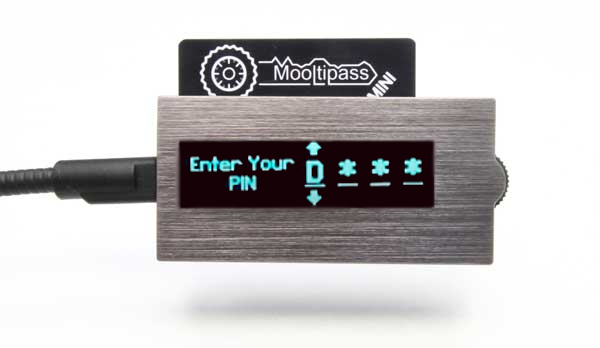
\includegraphics[width=0.6\columnwidth]{chapters/figures/related/mooltipass.jpg}}
  \caption{The mooltipass device and smartcard}
  \label{fig:mool}
\end{figure}

Its use is very, simple, as explained in their official website \cite{mooltipass}:

``The Mooltipass is designed to be as simple as possible to use for users of all backgrounds and ages:
\begin{enumerate}
\setlength\itemsep{0pt}
\item Plug the Mooltipass to your computer/tablet/phone. No driver is required
\item Insert your smartcard, unlock it with your PIN. Without the PIN, the card is useless.
\item Visit a website that needs a login. If using our browser plugin, the Mooltipass asks your permission to send the stored credentials, or asks you to save new ones if you are logging in for the first time.
\item If you are not using the browser plugin or are logging in on something other than a browser, you can tell the Mooltipass to type your logins and passwords for you, just like a keyboard.
\end{enumerate}

The Mooltipass emulates a standard USB keyboard, and can therefore type your passwords for you on Windows, Linux, Mac and even most Apple and Android devices (through the USB On-The-Go port). It doesn't need any special drivers to function. ''

The browser plugins offer a GUI where the user see and manage their passwords, as shown in Figure \ref{fig:mpapp}

\begin{figure}[htb]
  \centering
  \captionsetup{justification=centering}
  \centerline{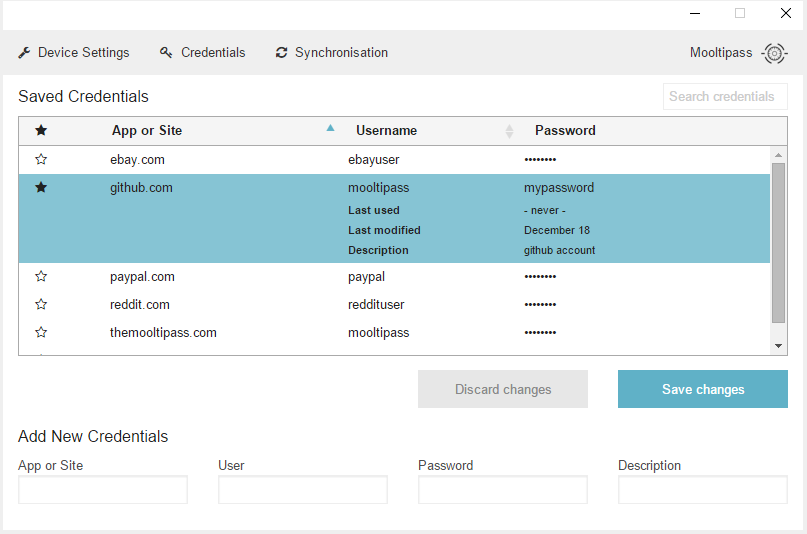
\includegraphics[width=0.9\columnwidth]{chapters/figures/related/mpapp.png}}
  \caption{The mooltipass application}
  \label{fig:mpapp}
\end{figure}

The Mooltipass works by storing an encrypted version of the passwords, and allowing their decryption only when the proper smartcard is connected and the correct pin introduced. From the website:

``The Mooltipass has an internal flash in which the user encrypted credentials are stored, while a PIN-locked smartcard contains the AES-256bits key required for their decryption. Like any chip and pin card, 3 false tries will permanently disable the Mooltipass card. Credentials are sent over HID, any password accessing operation needs to be physically approved by the user on the device.''

Mooltipass is open software and open hardware. In fact they encourage the community to develop and review code, so that the system's reliability is increased. Their GitHub repository host all the sources from the beginning of the project. \cite{mpgit}.

The Mooltipass project started off as a Hackday post from developer Mathieu Stephan, that gained enough recognition by the community to be founded by a kickstarter campaign. The Hackday project website \cite{mphack} contains more details regarding the hardware implementation:

\begin{itemize}
\setlength\itemsep{0pt}
\item \textbf{ST662ACD-TR:} Power Management
\item \textbf{ATMEGA32U4-MU:} Arduino compatible Microprocessor
\item \textbf{AT88SC102:} Secure Memory Smart Card
\item \textbf{AT45DB011D-SSH-T:} FLASH Memory
\end{itemize}

Figure \ref{fig:mparchi} shows the basic architecture.
\begin{figure}[htb]
  \centering
  \captionsetup{justification=centering}
  \centerline{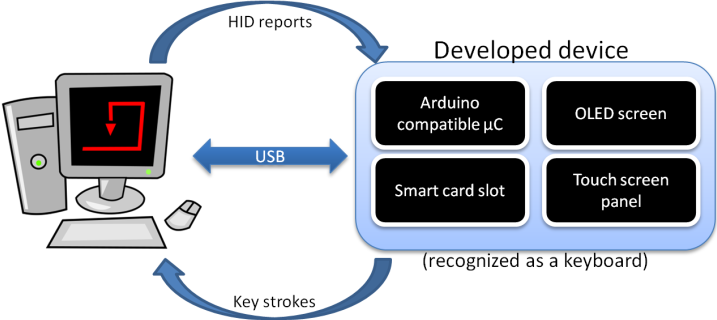
\includegraphics[width=0.9\columnwidth]{chapters/figures/related/mparchi.png}}
  \caption{The Mooltipass basic architecture}
  \label{fig:mparchi}
\end{figure}

In conclusion, mooltipass is a mature project that follows the same idea developed in this work: Guarantee the security of a set of passwords by allowing their decryption only through the use of a hardware device that the user will carry with them, hopefully, all the time. However there are some important difference between their system and SEcubeWallet:
\begin{enumerate}
\setlength\itemsep{0pt}
\item SEcubeWallet is based on the SEcube™ platform, making it much more trustworthy and robust, as this is a platform even used in military applications, and has been tested in the most demanding conditions.

\item Because SEcube™ integrates all the required security elements into one single chip, the final product is much more smaller (The size of a regular USB stick) than the mooltipass device.

\item Because the SEcube™ platform offers more possibilities for the development of applications, for example using the open source libraries, or the FPGA inside the chip, the SEcubeWallet can be extended or be integrated with other projects.

\item SEcubeWallet offers a couple of additional functionalities: Strong Password generation and entropy estimation, increasing the user experience.
\end{enumerate}

\section{SEcube™ based applications}

Before starting the application development, the following three projects were studied in order to familiarize with the SEcube™ framework and libraries usage. All of the projects make part of the SEfile SDK available at \cite{SEcubeRes} and are covered in details in the L2 user Manual \cite{L2UserMan}.

\subsection{Secure Text Editor and Secure Image Viewer}

This two projects are very similar, both use the SEcube™ framework, in particular the \texttt{SEfile} library, to encrypt/decrypt plain text files and images respectively. They are not intended to be final user applications, but demos that allow developers to learn how to use the SEcube™ libraries.

``Both these two projects have been developed in C++ with Qt libraries. They are based on 3
major security classes, in a one-to-one mapping with the 3 most important security opera-
tions: the first one manages the security platform to which the user wants to log in, the sec-
ond one allows the selection of the secure environment through the \texttt{secure\_update()} function, while the third one manages the opening and creation of files resorting on the \texttt{secure\_ls()}.''\citep{L2UserMan}.

The secure text editor, in short \texttt{SEfile\_TXT} offers the possibility to create/edit/open plain text documents, and generate an encrypted version of the file that will be stored in the same directory. ``It is possible to verify that encrypted files cannot be read properly from regular text editors; conversely, the Secure Text Editor can transparently read any encrypted file (decrypting also the file name) which content has not been altered and is, thus, trusted. Unauthenticated content (i.e., content not corresponding to the file signature) is, instead, discarded''.

The secure image viewer, in short \texttt{SEfile\_IMG} allows the user to open the most common image formats, PNG JPG/JPEG and BMP, and generates the encrypted version, which can only be opened using the same application.

Figure \ref{fig:sefiledem} depicts these two demo applications.

\begin{figure}[ht]
  \centering
  \subfloat[SEfile\_TXT demo application\label{}]{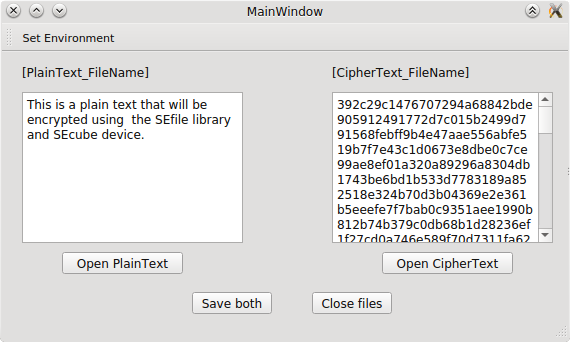
\includegraphics[width=0.48\textwidth]{chapters/figures/related/sefiletxt.png}}
  {}
  \subfloat[SEfile\_IMG\label{}]{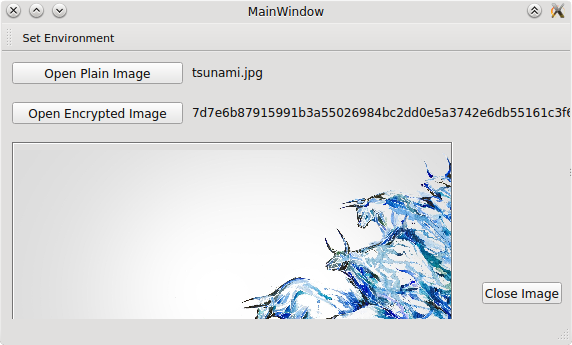
\includegraphics[width=0.48\textwidth]{chapters/figures/related/sefileimg.png}}
  \caption{SEfile demo applications}
 \label{fig:sefiledem}
\end{figure}

These two demo applications were used to learn the basis of the SEcube™ libraries, specially how to open the communication with the device, how to authenticate (login) and how to logout. The login dialogue used in the SEcubeWallet application is an improved version of these demos' login dialogue. The environmental dialogue was borrowed without any modification.

\subsection{secureSQLiteBrowser}

This application integrates the SEcube™ secureSQLite library with the DB Browser for SQLite\cite{SQLitebro} project, resulting in a powerful manager of encrypted SQLite databases.

The secureSQLite library, that makes part of the SEfile SDK, modifies the SQLite system to use the SEfile library in order to manage files, rather than using directly the OS calls. The result is a library that accepts all the standard SQLite commands, but stores the database as an encrypted file.

DB Browser for SQLite is an application developed in Qt that allows to manage SQLite DB from a powerful GUI. ``DB Browser for SQLite is a high quality, visual, open source tool to create, design, and edit database files compatible with SQLite. It is for users and developers wanting to create databases, search, and edit data. It uses a familiar spreadsheet-like interface, and you don't need to learn complicated SQL commands.'' \cite{SQLitebro}

By merging this two projects, the result is a wonderful application to create encrypted SQLite databases using an elegant and powerful GUI, depicted in figure \ref{fig:sqlitebro}, with tons of options, where the users can visually edit the DB tables, and store them as SEcube™ secured files. 

\begin{figure}[htb]
  \centering
  \captionsetup{justification=centering}
  \centerline{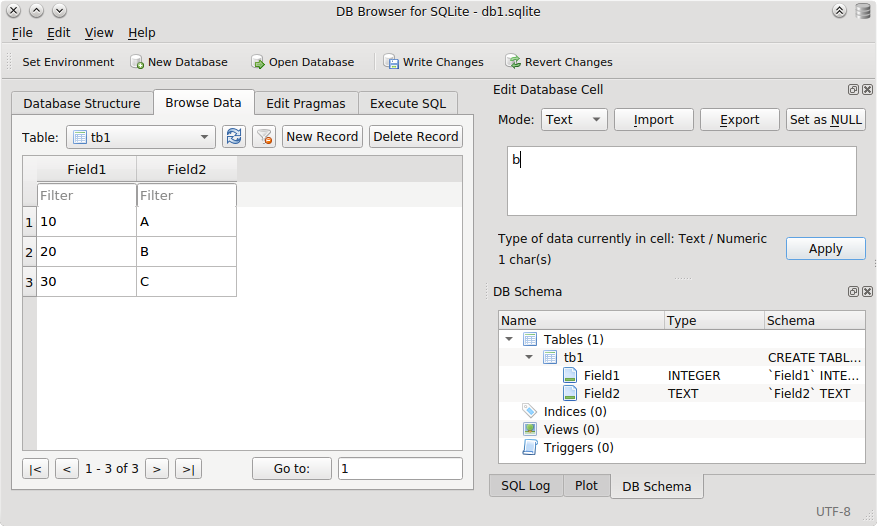
\includegraphics[width=1\columnwidth]{chapters/figures/related/sqlitebro.png}}
  \caption{secureSQLiteBrowser GUI}
  \label{fig:sqlitebro}
\end{figure}

Because SEcubeWallet is heavily based on the use of the secureSQLite library, this application was used to learn how to integrate the library into a Qt project. Additionally, it was used as inspiration for some of the GUI elements, like the filters above each column and the use of menus and toolbars. It was also use to diagnose the SEcubeWallet in the developing stage, by creating a DB with one application and opening it in the other. secureSQLiteBrowser could be use as a password manager in the sense that it can securely store and display wallets as tables, but it lacks the simplicity and additional functionalities that make SEcubeWallet attractive to users.




























\chapter{Frameworks, Libraries and software tools} \label{chap:lib}

As explained previously, the core of the design is the use of the SEcube™ chip as device to perform security operations in order to encrypt/decrypt some data stored in the host (PC). The requests to the device are made from the C/C++/Qt application developed in this work, which runs in the host machine. Said application exploits the existing C libraries SEfile and secureSQLite from the SEcube™ framework to ease the communication with the device. The chip firmware, written in C, is done using the Eclipse IDE. Additionally, the application uses of the random password generator PwGen and the password strength estimator zxcvbn, both of them open source libraries. A passphrase generator function was also developed and to keep some order it is treated as a library.

In the following sections a review of the SEcube™ platform's hardware and software components is given. Then a brief explanation of the C/C++/Qt framework and why it was chosen. Finally the additional software tools and libraries are presented.

\section{The SEcube™ framework}

``The SEcube™ (Secure Environment cube) Open Security Platform is an open source security oriented hardware and software platform, designed and constructed with ease of integration and service-orientation in mind. The hardware part of the platform was originally designed by Blu5 Group \cite{Blu5}, whereas the software libraries stem from a strong cooperation among international research institutions.'' \cite{GetStart}.

\vspace{5pt}

The main \textbf{hardware} products, explained in detail in the following sections, are:
\begin{itemize}
\setlength\itemsep{0pt}
\item The Chip, named SEcube™ Chip, or simply \textbf{SEcube™}
\item The Development Board, named \textbf{SEcube™ DevKit}
\item The USB Stick, named \textbf{USEcube Stick}.
\end{itemize}

The SEcube™ chip is the main hardware component, and both the devkit and USB Stick are designed around it.The Development Board provides several communication protocols as well as debugging capabilities. For the final product the board would be of course too inconvenient to carry, and instead the USEcube Stick is preferred.

\subsection{The SEcube™ Chip}

``The SEcube™ (Secure Environment cube) is a powerful chip which
integrates three key security elements in a single package. A fast
floating-point Cortex-M4 \textbf{CPU}, a high-performance \textbf{FPGA} and an
EAL5+ certified Security Controller (\textbf{Smart Card}).
The result of this innovative combination gives an extremely
versatile secure environment in a single SoC, in which developers
can rapidly implement complex applications and appliances.
... The SEcube™ is the ultimate solution for high-end design,
delivering integration of a flexible, configurable and certified
secure element.'' \cite{SEcubeDS}

We can then see the SEcube™ chip as a powerful device offering the flexibility of an \textsc{ARM} CPU, the speed of an FPGA and the reliable security of a certified Smart Card, all bounded together and easily integrated in any project thanks to the available communication protocols, among them USB, UART, Ethernet and JTAG. 

The chip includes a true random number generator which relies in 240 noise seeds, all physical and therefore unpredictable. This allows the creation of true random noise. Additionally the user can choose what type of noise they want to generate, for instance white or Fourier noise.

%TODO
\todo{talk more about cpu, low power modes...}

In figure \ref{fig:SEcubeBD} a simplified SEcube™ architecture is shown.

\begin{figure}[ht]
	\centering
	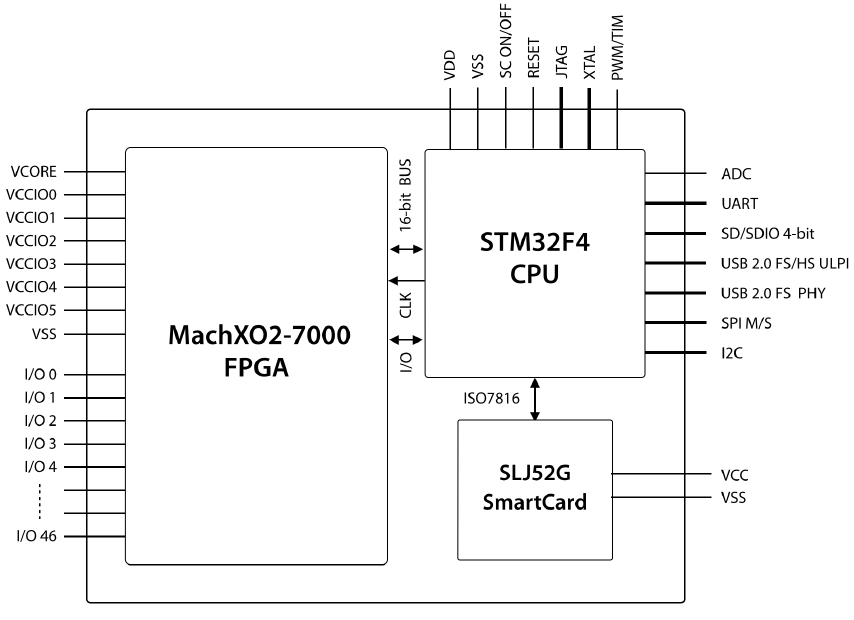
\includegraphics[width=\textwidth]{chapters/figures/development/SEcubeBlocks.png}
	\caption{SEcube™ Block Diagram}
	\label{fig:SEcubeBD}
\end{figure}


\subsection{Development board: The SEcube™ DevKit}

The development board integrates the SEcube™ chip with several peripherals that allow the user to easily communicate, program and debug. (Figure \ref{fig:devboard})

\begin{figure}[ht]
  \centering
  \subfloat[]{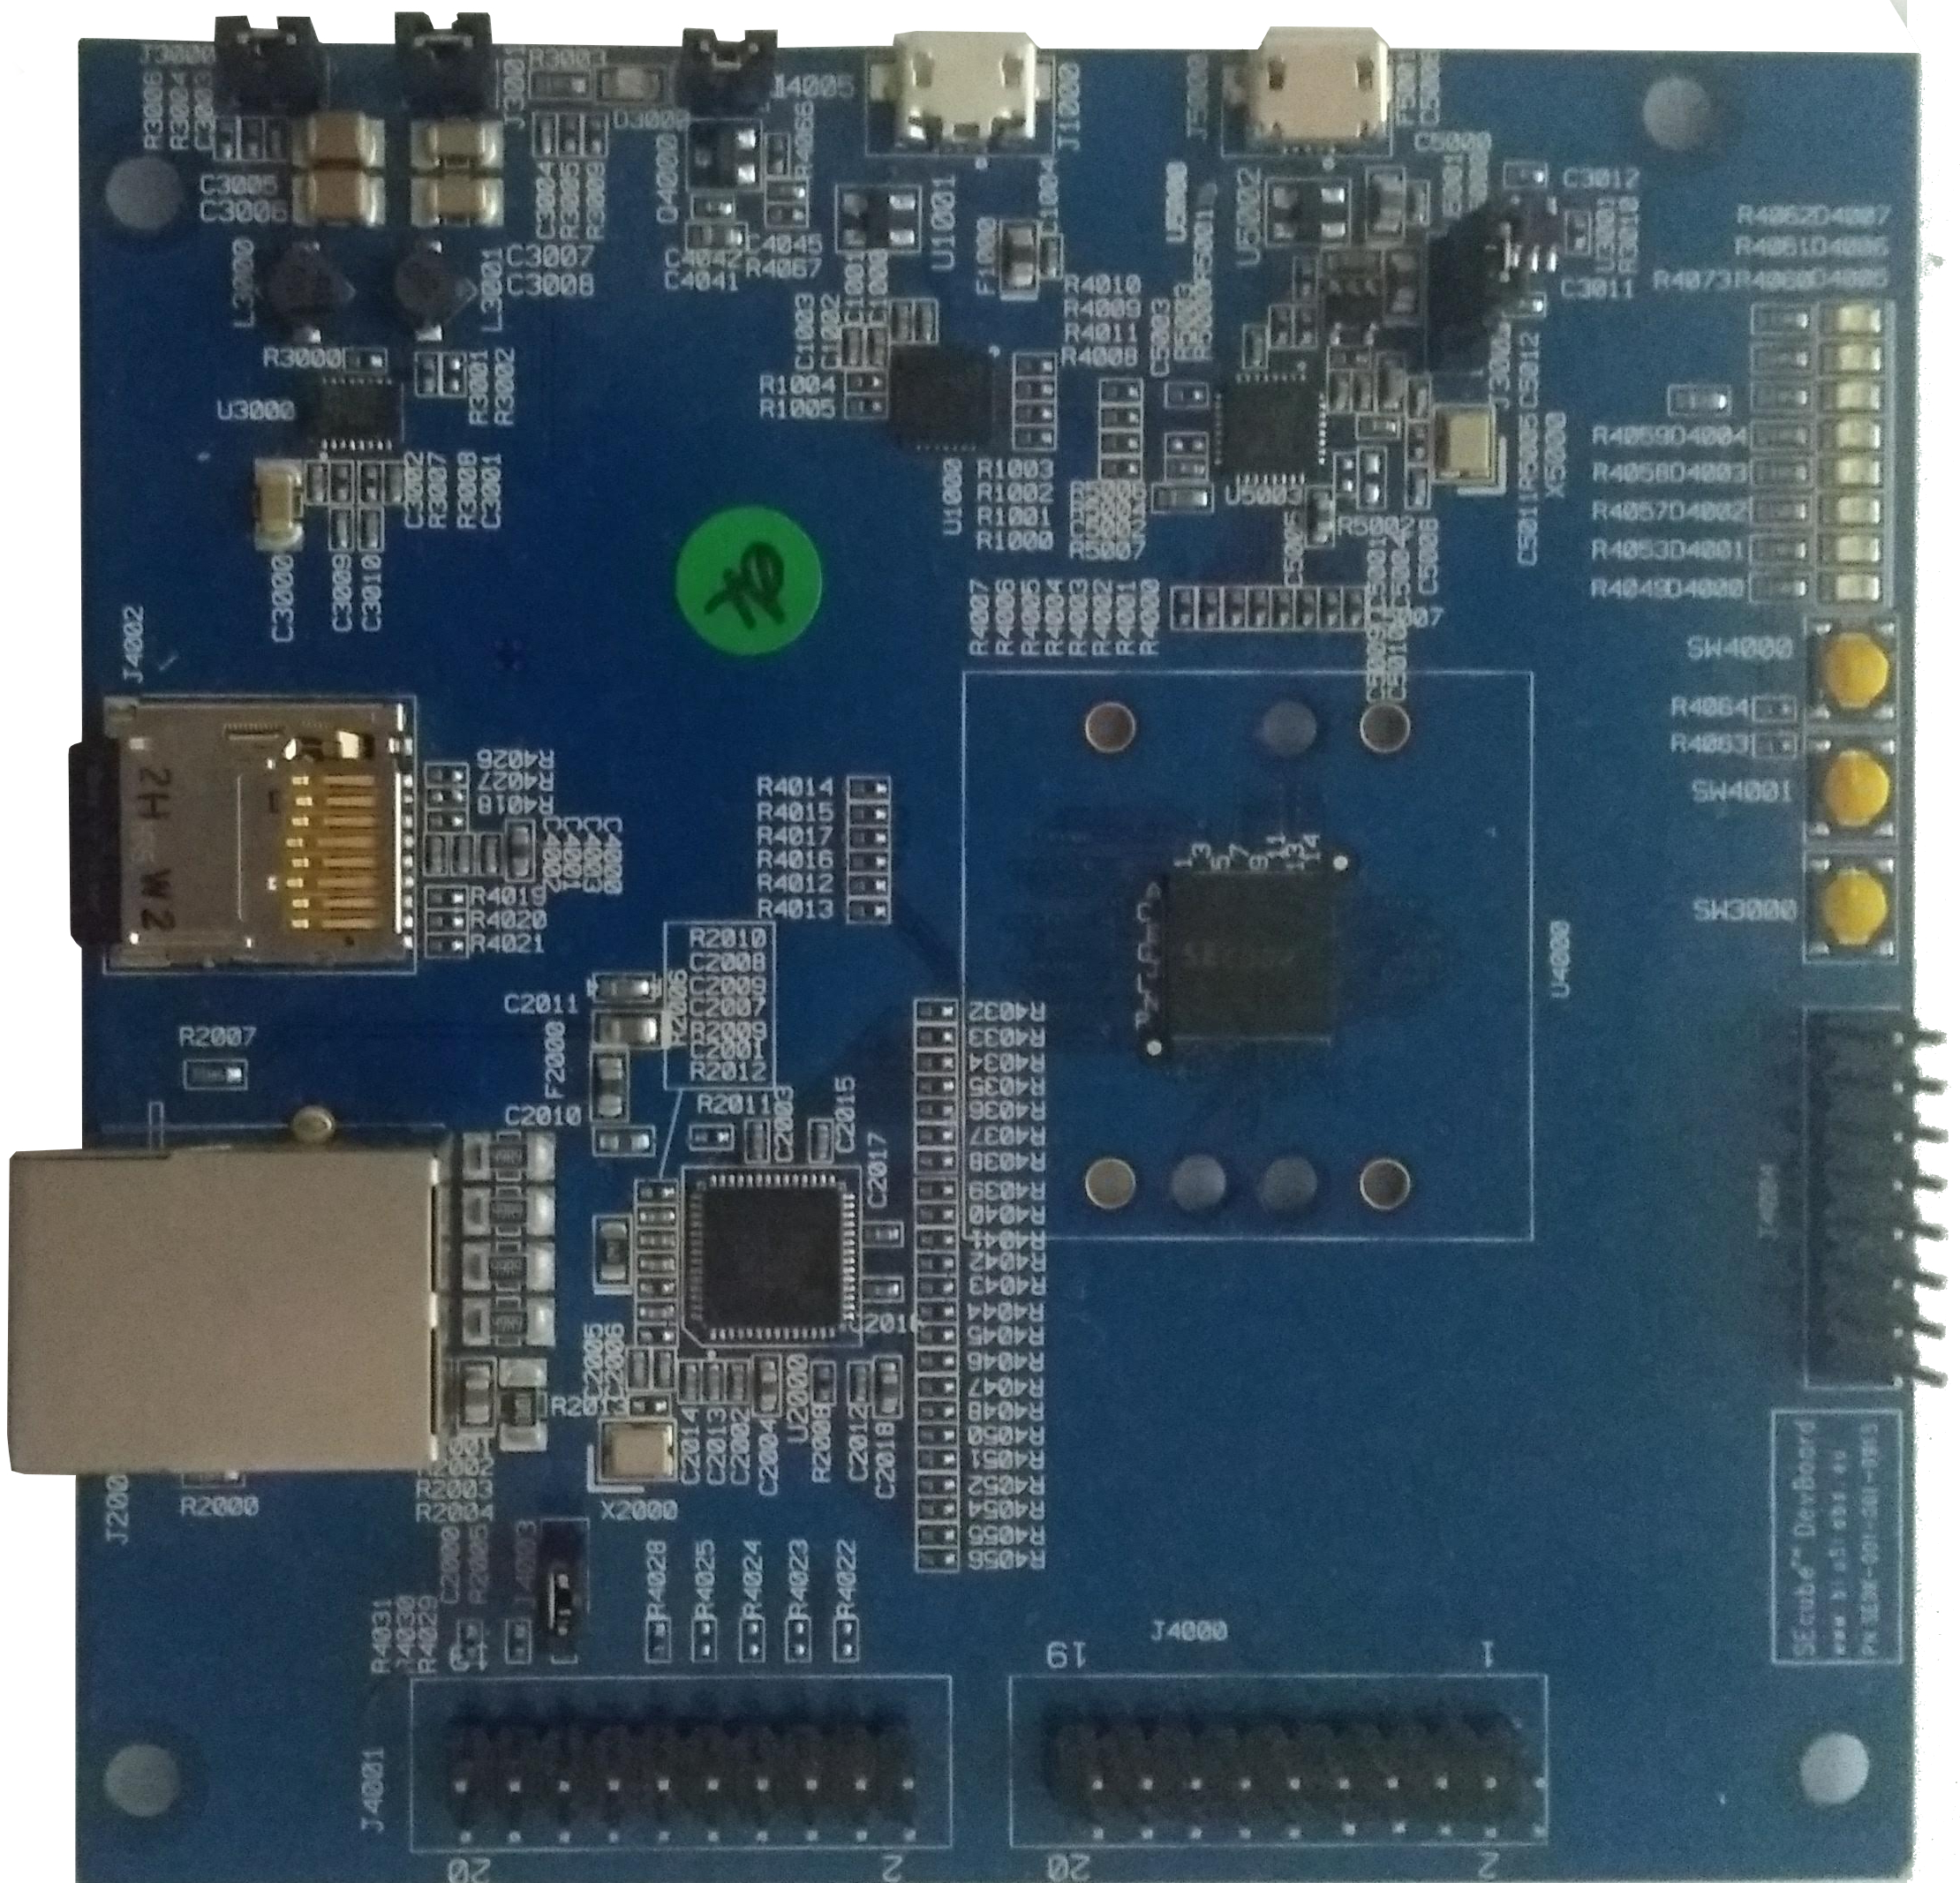
\includegraphics[width=0.485\textwidth]{chapters/figures/development/devboard.jpg}}
  \subfloat[]{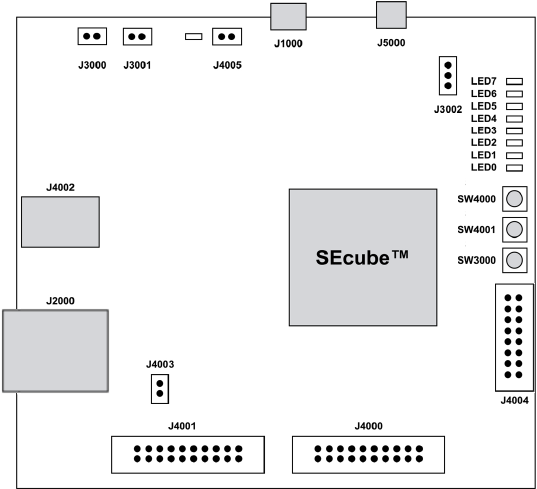
\includegraphics[width=0.515\textwidth]{chapters/figures/development/devboard_sch.png}}
  \caption{SEcube™ Devkit}
 \label{fig:devboard}
\end{figure}

The main peripherals in the SEcube™ devkit are:

\begin{itemize}
\setlength\itemsep{-3pt}
\item \textbf{J1000: }\tabto{2.3cm} USB 2.0 to UART 
\item \textbf{J2000: }\tabto{2.3cm} Ethernet 10/100 socket 
\item \textbf{J4000: }\tabto{2.3cm} SEcube™ embedded FPGA and CPU GPIOs
\item \textbf{J4001: }\tabto{2.3cm} SEcube™ embedded CPU JTAG
\item \textbf{J4002: }\tabto{2.3cm} microSD card 
\item \textbf{J4004: }\tabto{2.3cm} SEcube™ embedded FPGA and CPU GPIOs
\item \textbf{J5000: }\tabto{2.3cm} USB 2.0 High Speed 
\item \textbf{LEDx:  }\tabto{2.3cm} Leds 
\item \textbf{SWx00y:}\tabto{2.3cm} Switches 
\end{itemize}

\subsection{Final product: USEcube Stick}

For the final product, its is desired that the user carries all the SEcube™ functionalities in a small and convenient package, so they can encrypt/decrypt the passwords in any PC by just connecting the USEcube Stick and running the SEcubeWallet application.

The USEcube Stick is compatible with any Operating System and the SEcube™ functionalities are easily exposed to applications and services without installing any driver.

The USEcube offers only the strictly required components: The SEcube™ chip, a USB 2.0 High-Speed interface and an SDcard socket. See Figure \ref{fig:USEcube} for more details.


Since the USEcube Stick storage capability is based on a external microSD card, the security of the system is improved, as this allows to have a separation of encrypted data from the encryptor/decryptor. Additionally, both the size and the speed can be tuned per the user requirement and can be changed at any time, just replacing the microSD, without buying a new USEcube Stick.
The microSD card socket is embedded in the USB connector allowing to save space making the USEcube Stick very compact and, at the same time dust
and water-resistant.
Since the USEcube Stick is not provided with the JTAG interface, to inject the firmware previously developed and tested on the SEcube™ DevKit, all the devices come with an embedded secure boot loader.


\begin{figure}[ht]
  \centering
  \subfloat[]{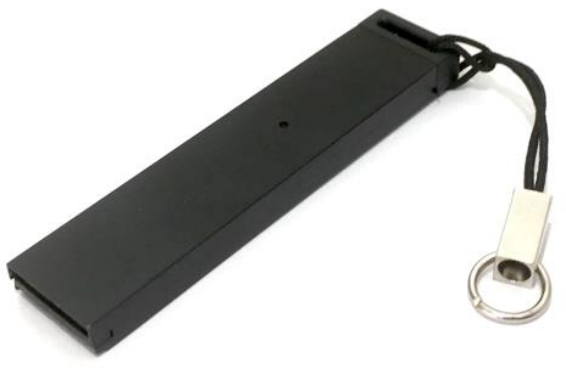
\includegraphics[width=0.485\textwidth]{chapters/figures/development/usb.png}}
  \subfloat[]{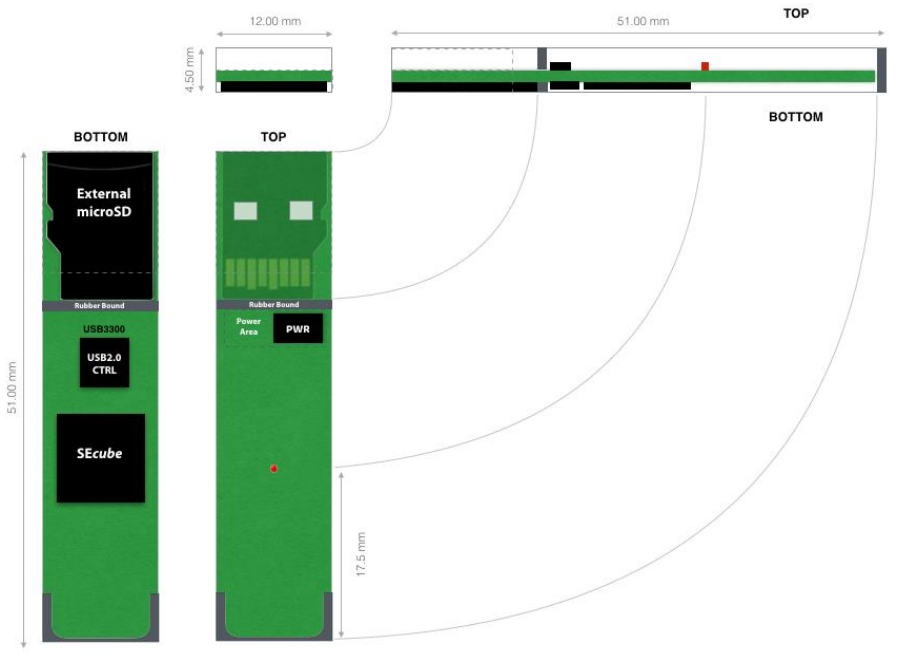
\includegraphics[width=0.515\textwidth]{chapters/figures/development/usb_sch.png}}
  \caption{USEcube Stick}
 \label{fig:USEcube}
\end{figure}

\subsection{SEcube™ Open SDK}

The SEcube™ Open SDK available at \cite{SEcubeRes} is a set of libraries, for both the SEcube™ device and the host machine. In general, the user interacts with the host libraries requesting security services. The host in turn pass those request to the device libraries, which are the ones that actually execute any security algorithms. The results are passed back to the host and ultimately to the user.

``The software libraries and design environment allow developers who are not willing or able to produce the security APIs and protocols themselves to exploit the ready functions provided (currently as APIs and soon as services) within the SEcube™ platform and experience the platform as a high-security black box.'' \cite{L2UserMan}

``From the user/developer point of view, the APIs have been implemented targeting two
nested environments depending on where physically the code runs:
\begin{itemize}
\setlength\itemsep{1pt}
\item \textbf{Device-Side}, including the libraries of basic functionalities that are executed on the embedded processor of the SEcube™-based hardware device.
\item \textbf{Host-Side}, containing libraries of functions executed on the host PC and interface functions for calling services and processes residing on the embedded processor of the SEcube™ device.
\end{itemize} 

From the architectural point of view, the Host-Side Libraries have been implemented targeting 4 hierarchical abstraction levels, and namely:
\begin{itemize}
\setlength\itemsep{-3pt}
\item \textbf{Level 0:} Communication Protocol and Provisioning APIs
\item \textbf{Level 1:} Basic Security APIs
\item \textbf{Level 2:} Intermediate Security APIs
\item \textbf{Level 3:} Advanced Security APIs
\end{itemize}

At each level, each component represents a "service" for the upper level and relies on "services" provided by the next lower level, only.'' \cite{L2UserMan}

The Device-Side Libraries only have the lower two levels of abstraction, and each of these levels communicates with its host-side counterpart.

In Figure \ref{fig:levels} a graphical representation of the hierarchical levels is presented. For each level is shown, in parenthesis, an example of a function/application belonging to it.

\begin{figure}[htb]
  \centering
  \captionsetup{justification=centering}
  \centerline{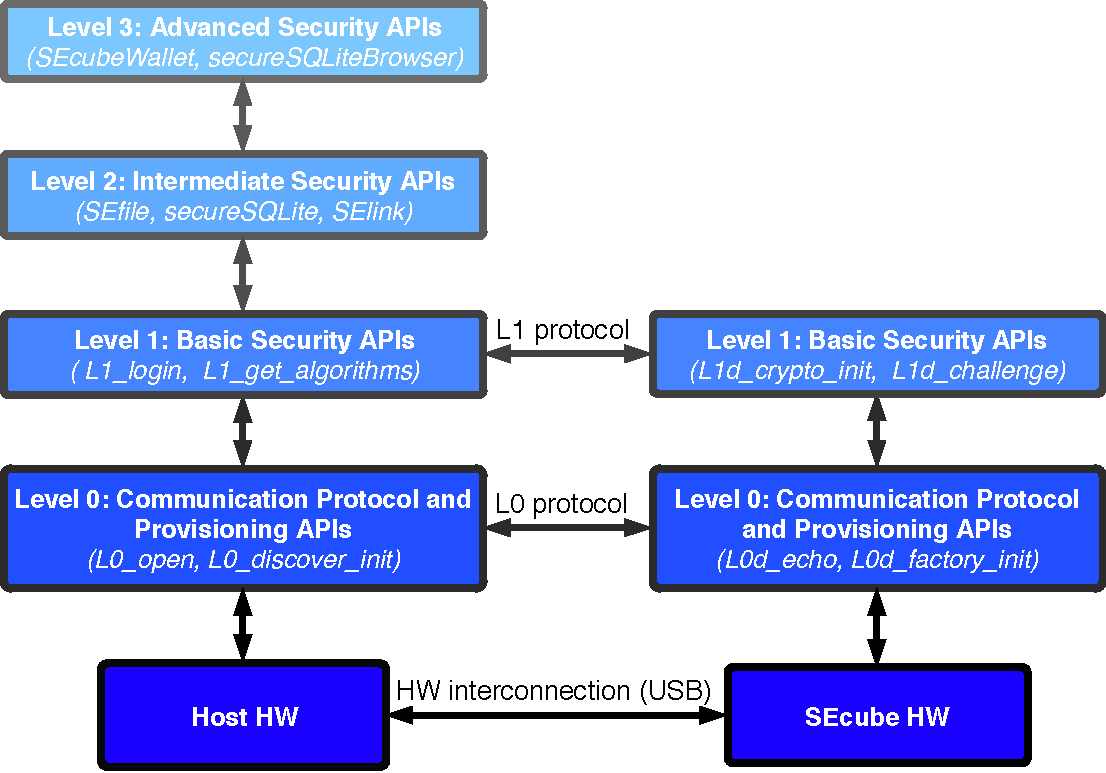
\includegraphics[width=\columnwidth]{chapters/figures/frameworks/levels.pdf}}
  \caption{Libraries Hierarchy Levels}
  \label{fig:levels}
\end{figure}

\subsection{Level 2: Intermediate Security APIs}

SEcubeWallet is a Level 3 application that relies heavily on the Level 2 APIs SEfile and secureSQLite. In this section a review of these APIs is given.

``Level L2 relies on L1 services to provide the APIs for implementing more abstract secure functionalities. Typical examples include APIs for the protection of data both at rest and in-motion, or negotiating parameters (e.g., keys, algorithms) for establishing secure sessions, without being forced to understand in details all the low-level hardware and security mechanisms.''\cite{L2UserMan}

L2 can be considered as the merge of two projects: \textbf{SEfile}, concerning data at rest, and \textbf{SElink}, concerning instead data at motion. 

\subsection{SEfile}

``SEfile targets any user that, by moving inside a secure environment, wants to perform basic operation on regular files. It must be pointed out that all encryption functionalities are demanded to the secure device in their entirety. In addition, SEfile does not expose to the host device details about what, or where it is reading/writing data: thus, the host OS, which might be untrusted, is totally unaware of what it is writing''. \cite{L2UserMan}.


A secured file has the structure shown in figure \ref{fig:secfile}. The data is divided in sectors, and each of them is encrypted and signed. The first sector does not contain data, but metadata on the file itself, and it is known as the header.

When a portion of the file wants to be read or written (i.e. encrypted or decrypted), it is not necessary to process the whole file. Only the required sectors are manipulated, thus reducing the overhead time of securing operations.

\begin{figure}[htb]
  \centering
  \captionsetup{justification=centering}
  \centerline{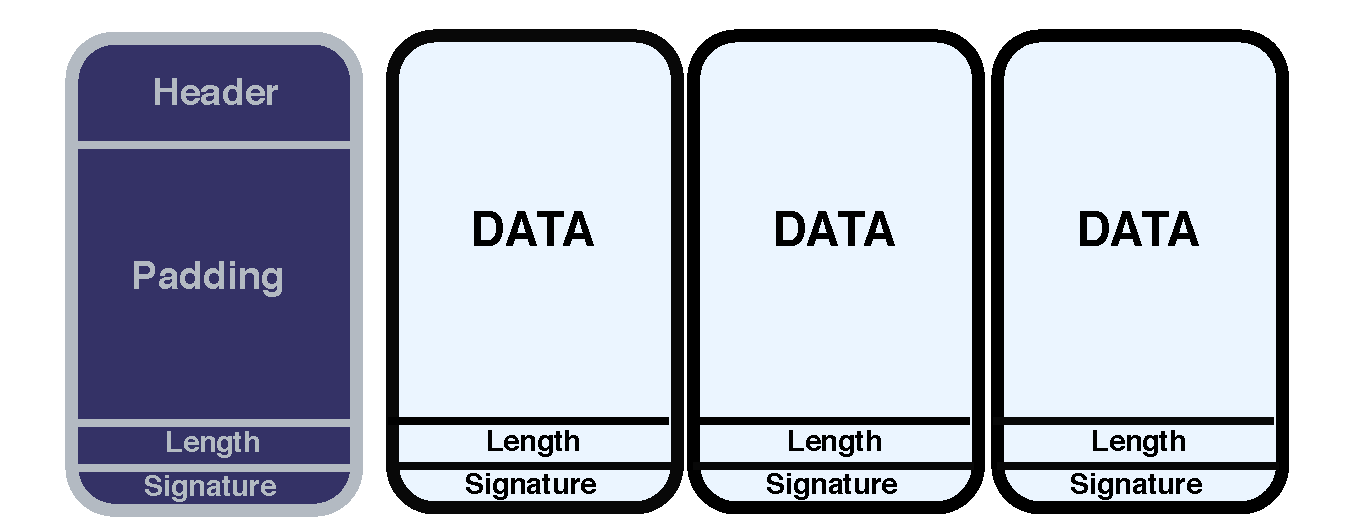
\includegraphics[width=1\columnwidth]{chapters/figures/frameworks/secfile.pdf}}
  \caption{Secure File structure}
  \label{fig:secfile}
\end{figure}

For file encryption, SEfile uses The Advanced Encryption Standard (AES), established by the U.S. National Institute of Standards and Technology (NIST). For each data sector AES-256-CTR is used, while the header sector is encrypted using AES-256-ECB.

For authentication, ``each sector, including the header, is signed using an authenticated signature obtained with SHA-256-HMAC, meaning that the signature depends on both the data contained in the sector itself and on a chosen encryption key. To use two different keys to encrypt data and to digest authentication, a feature increasing overall system security, SEfile leverages on the pbkdf2() function already implemented within the SDK.''\cite{L2UserMan}


\subsection{secureSQLite}

Based on the SQLite data base management system, and using SEfile, this API allows the user to create SEcube™ secured data bases.
``Leveraging on its modularity, the SQLite system has been modified to resort on a custom functionalities wrapper based on SEfile, rather than using directly the OS calls. The starting point of this work was the template offered as example for making a custom VFS interface distributed along with SQLite, version 3.13.0.''\cite{L2UserMan}

Every database created with secureSQLite is cyphered and signed up to its file name before being stored, thus making it impossible to read the database contents without authenticating and using the library.

\section{SQLite Data Base management system}
A Data Base is a structured set of data stored and accessed electronically using a data base management system. 

SQLite \cite{SQLite} is one of such management systems. It implements most of the SQL (Structured Query Language) standard. Unlike most other SQL databases, it is serverless, meaning there is not separate server process, and an application can access directly the database file without the need of interprocess communication. SQLite is ACID (Atomicity, Consistency, Isolation, Durability) compliant, meaning database transactions are valid even in case of errors, leading to program crashes, OS crashes or power failures. It can run in any operating system, even embedded ones. SQLite is implemented in generic C, and it is self-contained in a C library, meaning it has very few dependencies and all the code is encapsulated single source code file. 

In this work the Qt SQLite plugin was used to manage the in-memory SQLite databases. ``The Qt SQLite plugin makes it possible to access SQLite databases\dots SQLite operates on a single file, which must be set as the database name when opening a connection. If the file does not exist, SQLite will try to create it. SQLite also supports in-memory and temporary databases. Simply pass respectively ":memory:" or an empty string as the database name.'' \cite{qsqlite}.

\section{Graphical User Interface: the Qt framework}
The application's graphical user interface was developed using the \textbf{Qt framework}, version 5.11.1, available for download at \cite{qtdown}. (Qt 5.10 or higher is required to compile the sources of this project, as it uses the \texttt{QRandomGenerator} Class included in that version).

``Qt is a cross-platform application development framework for desktop, embedded and mobile. Supported Platforms include Linux, OS X, Windows, VxWorks, QNX, Android, iOS, BlackBerry, Sailfish OS and others. Qt is not a programming language on its own. It is a framework written in C++. A preprocessor, the MOC (Meta-Object Compiler), is used to extend the C++ language with features like signals and slots. Before the compilation step, the MOC parses the source files written in Qt-extended C++ and generates standard compliant C++ sources from them. Thus the framework itself and applications/libraries using it can be compiled by any standard compliant C++ compiler like Clang, GCC, ICC, MinGW and MSVC''.\cite{Qt}  


For writing, compiling and debugging source code, the IDE \textbf{Qt Creator}, version 4.6.2 was used.

``Qt Creator provides a cross-platform, complete integrated development environment (IDE) for application developers to create applications for multiple desktop, embedded, and mobile device platforms, such as Android and iOS. It is available for Linux, macOS and Windows operating systems''.\cite{QtC}.

\vspace{5pt}
The reasons behind the use of Qt are as follows:

\begin{itemize}
\setlength\itemsep{0pt}
\item Qt is a C++ library, and as such, allows for a seamless use of the C libraries SEfile and secureSQLite, which are the backbone of this project.

\item Qt is cross-platform, meaning the developed application can be compiled to work on any of the major OSes. In particular, the development was carried out an tested on a Linux machine, but the application should work with no problems in Windows and MacOS. 

\item Because of good designed and ready-to-use display items such as tables, menus and dialogues, it is possible to focus in writing the functional portions of the application without worrying too much about the GUI. And as it is open source, any Qt item can be modified and extended when it does not meet the expectations out of the box. In this project several display elements were improved, as will be seen in section \ref{sec:imp}.

\item Thanks to the multitude of functions dedicated to ease the use of C++ libraries and OS calls, one can be more productive, and the resulting code is more reliable. For instance, this project makes extensive use of such libraries, like QSqlDatabase, QString, QProcess, etc. Again, more details are given in section \ref{sec:imp}

\item The Related works described in section \ref{sec:relsecube}, secureSQLiteBrowser, SEfile\_TXT and SEfile\_IMG, are written in Qt.

\item Qt is widely used, meaning it is possible to find tons of documentation, forums and additional libraries on the web. This also ensures the Qt framework will have continuous support from the developers and the community.

\end{itemize}

\section{Device side development: Eclipse}

For device-side development, the Eclipse IDE for C/C++, version Neon.3 Release (4.6.3) \cite{eclipse} was used. 

Although this thesis work regards mostly host-side code development (i.e. the Qt application SEcubeWallet), it was necessary to do some slight modifications to the firmware running in the SEcube™ chip, as will be explained in details in section \ref{sec:authen}. 

Eclipse is the recommended IDE for SEcube™ firmware development, as stated in the Getting Started guide \cite{GetStart}. With Eclipse it is possible to perform all the operations required to effectively modify the code running inside the SEcube™ chip, namely write/modify the code, compile it, load it into the chip, and if necessary debug it. But because the code will run in an embedded system, more specifically in an ARM microprocessor, some additional tools and plugins are needed. 

In order to program and debug the chip, an ST-Link/V2 was used. The ST-Link/V2 is an professional tool to debug and program STM8 and STM32 MCUs. It communicates with the microcontroller using the JTAG/SWD connection present in the DevKit board, as see in figure \ref{fig:con}

\begin{figure}[ht]
  \centering
  \subfloat[]{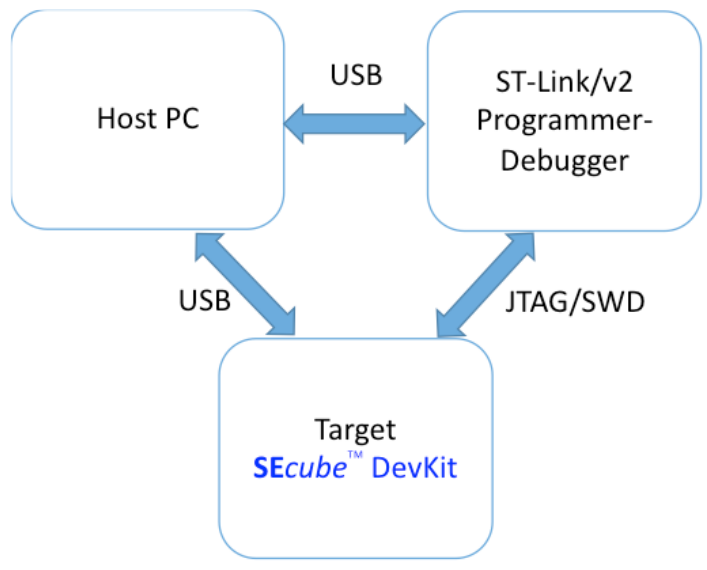
\includegraphics[width=0.48\textwidth]{chapters/figures/frameworks/conSche}}
  {}
  \subfloat[]{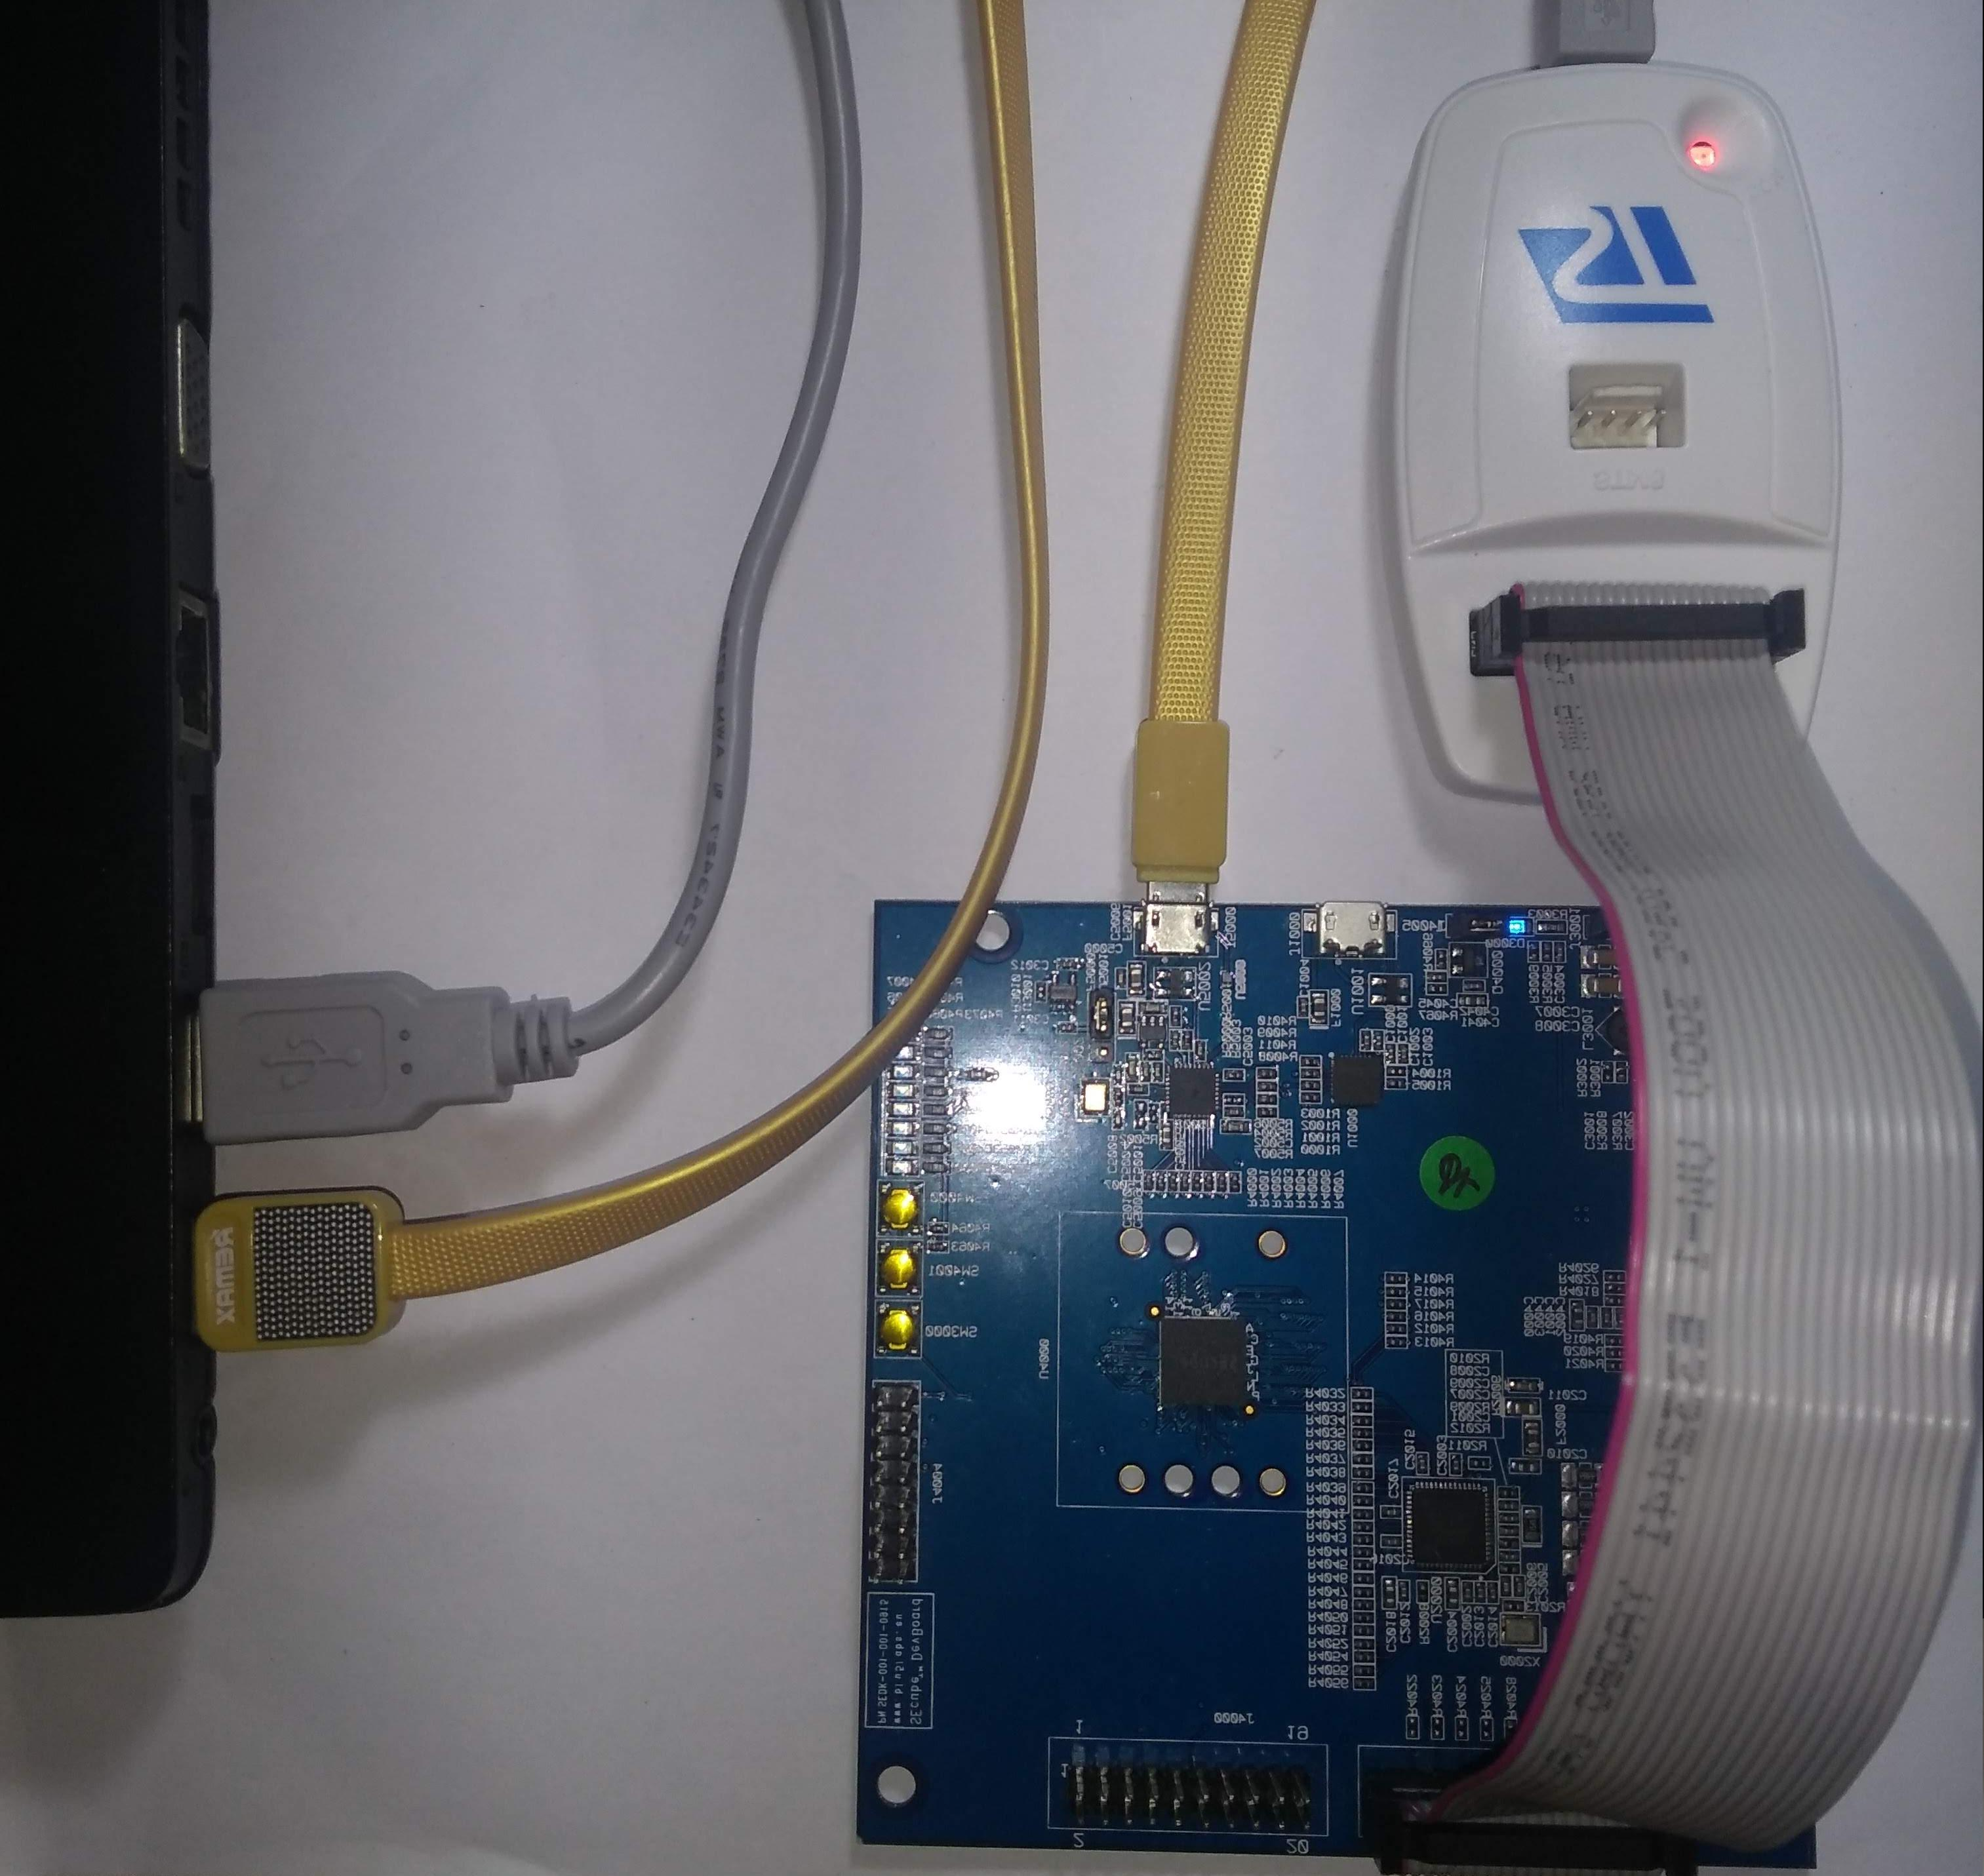
\includegraphics[width=0.48\textwidth]{chapters/figures/frameworks/conReal2}}
  \caption{DevKit and ST-Link/V2 connections to PC}
 \label{fig:con}
\end{figure}

The Getting Started guide does a very good job explaining in detail how to install all the necessary software. Here a brief recap of the followed steps is giving, plus some additional configurations that are required when running the IDE on Linux (In the author's case, Linux Mint 17.1, kernel 3.13.0-37).


\begin{enumerate}
\setlength\itemsep{0pt}
\item \textbf{Java Runtime Environment:} Necessary to run Eclipse, as it is a Java program. The version 1.8.0\_171 was installed, available at \cite{java}

\item \textbf{Eclipse:} Eclipse for C/C++, Neon version was used. Available at \cite{eclipse}

\item \textbf{AC6 Tools Eclipse Plugin: }  Embedded Toolchain for ARM, which includes the building tools (GCC-based ARM cross compiler, assembler and linker), OpenOCD (Open On-Chip Debugger) and GDB debugging tools. In Linux, OpenOCD allows the communication with the STLink-V2 and therefore, the debugging. Available at \cite{ac6}.

\item \textbf{STM32CubeMX: }This is a STM32Cube initialization code generator that includes standard toolchains and embedded software libraries and middleware components (e.g., Open-source TCP/IP stack, USB drivers, open-source FAT file system, open source RTOS). Available at \cite{cubemx}.

\item \textbf{udev rules (Linux Only): }On Linux, it is required to include the STLink-v2 device rules in the udev device manager. To do so, instead of writing them manually it is easier to use the rules already generated in the mcu-gnu-eclipse version of openocd available in \cite{mcu}. After downloading the appropriate version (*centos64.tgz for a 64 bits Linux machine), the \texttt{.tgz} file is extracted and the \texttt{60-openocd.rules} file copied into the \texttt{rules.d/} directory using the commands in listing \ref{lis:udev}:

\begin{lstlisting}[float=htb, basicstyle=\ttfamily, frame=tb, caption={Including STLink rules to udev manager in Linux}, label = {lis:udev}]
sudo cp /gnu-mcu-eclipse/openocd/0.10.0-8-20180512-1921/
contrib/60-openocd.rules  /etc/udev/rules.d/

sudo udevadm control --reload-rules
\end{lstlisting}


\item \textbf{SEcube™ Open SDK: }Finally, the Open SDK available at \cite{SEcubeRes} can be used. There is an already configured environment for development, in the zip file \texttt{SEcubeSDK\_GAF\_14gen2017/SEcube\_SDK/Development/ Environment.zip}. After extracting it, the folder \texttt{/Environment/ws} can be used as Eclipse workspace. This opens the current version of the SEcube™ firmware, that can be then modified and loaded into the chip.

\end{enumerate}




\section{PwGen: Pronounceable Password generator}

The most secure type of passwords are random ones. A random password sufficiently long is considered to be virtually unbreakable. But this rises two problems: First of all, humans are inherently bad at creating true random passwords. Second, a random password is not suited to be remembered or even used (as it probably is too annoying to type). These two reasons motivated the inclusion of a Password Generator.

pwgen is an open source program that generates human friendly passwords that are also secure. It is available in the official Linux repositories, and there is a Windows version as well, but in this work the source files where used.

``The pwgen program generates passwords which are designed to be easily memorized by humans, while being as secure as possible. Human-memorable passwords are never going to be as secure as completely completely random passwords. In particular, passwords generated by pwgen without the -s option should not be used in places where the password could be attacked via an off-line brute-force attack. On the other hand, completely randomly generated passwords have a tendency to be written down, and are subject to being compromised in that fashion'' \cite{pwgen}.

pwgen offers several options that can drastically change the type of generated password. Here is a list of the options available for users of SEcubeWallet:

\begin{itemize}
\setlength\itemsep{0pt}


\item \textbf{Length:} The desired length of the password. It is recommended to be at least 12 for non-random passwords and 8 for random ones.

\item \textbf{-0, no numerals:} 
Don't include numbers in the generated passwords. 

\item \textbf{-A, no capitalize:} 
Don't bother to include any capital letters in the generated passwords. 
    
\item \textbf{-B, ambiguous:}
Don't use characters that could be confused by the user when printed, such as 'l' and '1', or '0' or 'O'. This reduces the number of possible passwords significantly, and as such reduces the quality of the passwords. It may be useful for users who have bad vision, but in general use of this option is not recommended. 
    
\item \textbf{-c, capitalize:}
Include at least one capital letter in the password.

\item \textbf{-n, numerals:}
Include at least one number in the password.

\item \textbf{-s, secure:}
Generate completely random, hard-to-memorize passwords.

\item \textbf{-v, no vowels:}
Generate random passwords that do not contain vowels or numbers that might be mistaken for vowels. It provides less secure passwords to allow system administrators to not have to worry with random passwords accidentally contain offensive substrings. 

\item \textbf{-y, symbols:}
Include at least one special character in the password.
\end{itemize}

By default pwgen behaves as if the options \textbf{-nc} were used, that is, pronounceable passwords with at least 1 capital letter and 1 number.

The strongest passwords this program can generate are obtained with the options \textbf{-ys}, as it results in random passwords with special symbols. They are very hard to remember, and should only be used if the user is willing to open the SEcubeWallet application each time they need to use one of the password.


\section{zxcvbn: Password strength estimation} \label{sec:zxcvbnth}

An important feature to have in a password manager is the possibility to realistically estimate how strong a password is, i.e., how hard could it be for hackers to crack it, as there is no point in using the SEcube™ system to protect weak passwords, that could be easily guessed with brute force attacks. As it is out of the author expertise to write a reliable function to make this estimation, it was decided to use a trusted project developed during the dropbox hackweek event in 2012. The estimator called \textbf{zxcvbn} was originally written in JavaScript aiming for an easy integration with multiple web browsers and OS. Fortunately, the community ported the library to a wide variety of languages including Python, Ruby and C/C++. In this work the C++ implementation was used. The project is Open Source and available for free use on GitHub \cite{zxgit}.

zxcvbn is regarded by the community as one of the most reliable and mathematically advanced open source password estimators. In security forums and discussion it always pops out as an excellent tool, much better than other passwords estimators commonly used in web pages. In \cite{naked}, the author compares zxcvbn to other popular java meters and arrives to the conclusion that only zxcvbn is reliable enough to actually give an useful feedback.
In \cite{gen_est_eval}, the author makes an evaluation of several password generators and strength estimators. PwGen and zxcvbn, the two libraries used in this work, always give excellent results.

``For over 30 years, password requirements and feedback have largely remained a product of LUDS: counts of Lower- and Uppercase letters, Digits and Symbols. LUDS remains ubiquitous despite being a conclusively burdensome and ineffective security practice. zxcvbn is an alternative password strength estimator that is small, fast, and crucially no harder than LUDS to adopt. Using leaked passwords, we compare its estimations to the best of four modern guessing attacks and show it to be accurate and conservative at low magnitudes, suitable for mitigating online attacks. We find 1.5 MB of compressed storage is sufficient to accurately estimate the best-known guessing attacks up to 105 guesses, or 104 and 103 guesses, respectively, given 245 kB and 29 kB. zxcvbn can be adopted with 4 lines of code and downloaded in seconds. It runs in milliseconds and works as-is on web, iOS and Android''. \cite{zxpaper}

``People of course choose patterns — dictionary words, spatial patterns like \texttt{qwerty}, \texttt{asdf} or \texttt{zxcvbn}, repeats like \texttt{aaaaaaa}, sequences like \texttt{abcdef} or \texttt{654321}, or some combination of the above. For passwords with uppercase letters, odds are it’s the first letter that’s uppercase. Numbers and symbols are often predictable as well: \texttt{l33t} speak (3 for e, 0 for o, @ or 4 for a), years, dates, zip codes, and so on.
As a result, simplistic strength estimation gives bad advice. Without checking for common patterns, the practice of encouraging numbers and symbols means encouraging passwords that might only be slightly harder for a computer to crack, and yet frustratingly harder for a human to remember. xkcd nailed it''. (see figure \ref{fig:xkcd}). \cite{zxdropbox}

\begin{figure}[htb]
  \centering
  \captionsetup{justification=centering}
  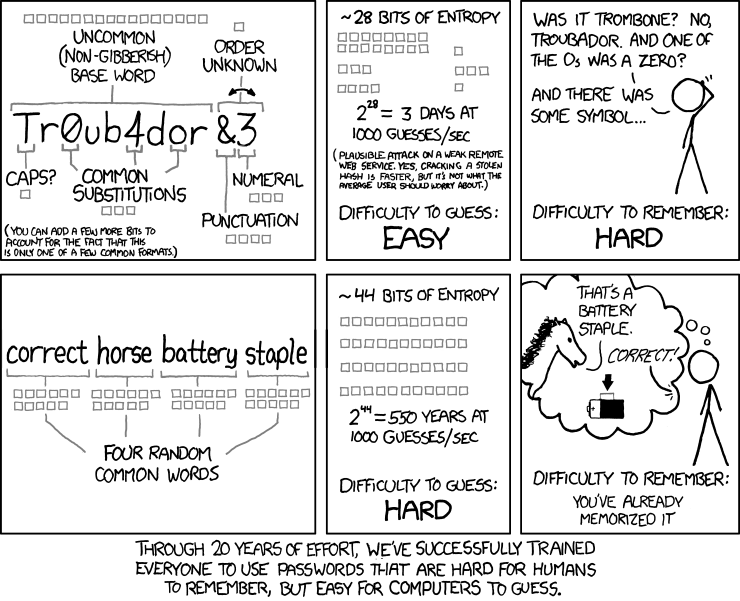
\includegraphics[width=\columnwidth]{chapters/figures/development/xkcd.png}
  \caption{Password strength, xkcd \cite{xkcd}}
  \label{fig:xkcd}
\end{figure}

To put it in other words, the authors of the project argue that a password like \texttt{correcthorsebatterystaple} (a nonsense English phrase) is more strong than a password like \texttt{Tr0ub4dour\&3}, even if the former does not have any upper cases or numbers, and the latter seems more complicated.

\begin{figure}[htb]
  \centering
  \captionsetup{justification=centering}
  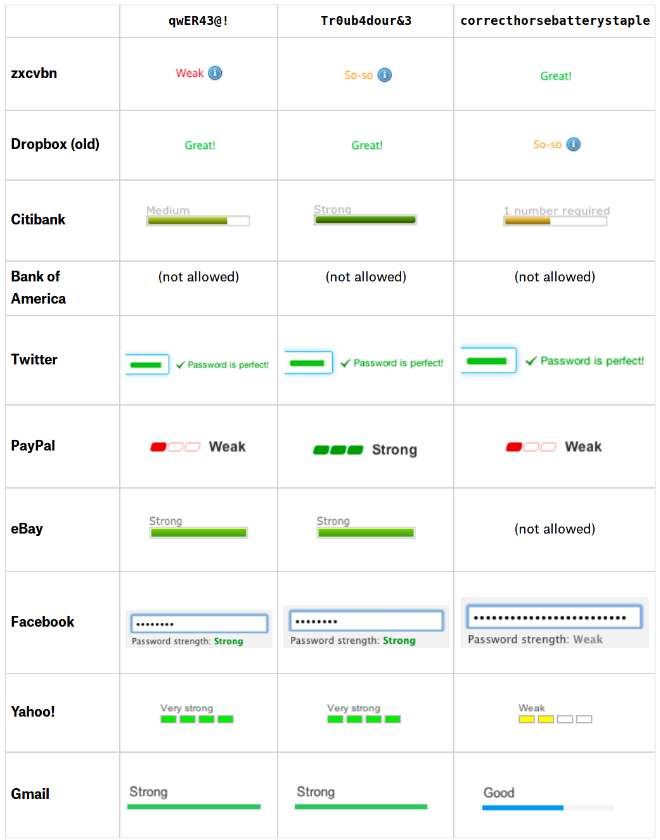
\includegraphics[width=\columnwidth]{chapters/figures/development/zxcvbn_comp.png}
  \caption{comparison between zxcvbn and popular websites' strength meters}
  \label{fig:tablez}
\end{figure}

The table in figure \ref{fig:tablez} (taken from \cite{zxdropbox}), show how zxcvbn is different from strength meters used in popular web services. (disclaimer: The data in the table is from 2012). From it we can learn:

\begin{enumerate}
\setlength\itemsep{-3pt}

\item Passwords like \texttt{\textbf{qwER43@!}}, which is a spatial password: it uses the keys \texttt{qwer4321}, with shift pressed for the keys \texttt{er} and \texttt{21} (the \texttt{@} symbol in the English keyboard is \texttt{shift+2}), is not considered week by most of the meters, but it should. It is probably due to the fact that it includes a combination of numbers and symbols that makes it look strong, but in reality, because of keyboard spatiality, is not.

\item Passwords like \texttt{\textbf{Tr0ub4dour\&3}}, which is generated by replacing some of Troubadour letters with numbers, and adding two more characters, is regarded as a very strong password for all of the meters except zxcvbn. Even if the base word is uncommon, and it has some variations, it is not long enough to be considered so strong.
\item A password like \texttt{\textbf{correcthorsebatterystaple}} is not considered strong by most of the meters except zxcvbn, and it is not even allowed in some cases because it lacks numbers, Upper-cases or symbols.
\end{enumerate}

The superiority of zxcvbn over the other meters in the table may seem like cherry picking, but the way zxcvbn is constructed explains these differences.

\subsubsection*{Matching}

Enumerates all the (possibly overlapping) patterns it can detect. Currently zxcvbn matches against:

\begin{itemize}
\setlength\itemsep{-3pt}


\item \textbf{Dictionaries:} Common words the user is likely to use as password. Multiple dictionaries, in a simple .txt format can be used. In this work, we present a few: English words, Italian words, names and surnames, Burnett’s 10,000 common passwords, words from tv and films. The match has an associated frequency rank, where words like the and good have low rank, and words like photojournalist and maelstrom have high rank. This lets zxcvbn scale the calculation to an appropriate dictionary size on the fly, because if a password contains only common words, a cracker can succeed with a smaller dictionary. For all dictionaries, match recognizes uppercasing and common \texttt{l33t} substitutions.

\item \textbf{Spatial keyboard patterns:} Some users are likely to choose passwords based on spatial pattern. For instance a user could choose the first row of letters from right to left: \texttt{poiuytrewq} as they password. \textsc{qwerty} keyboard, Dvorak keyboard, and keypad are considered.

\item \textbf{Repeats}: Users are also prone to use repetition of characters, like \texttt{rrrr}. 

\item \textbf{sequences}: Numeric or alphabetic sequences like \texttt{123} or \texttt{fedcba}

\item \textbf{years and dates}: The year or full date of a special event, like anniversary or birthday. Years from 1900 to 2019 are considered and dates in different formats. (3-13-1997, 13.3.1997, 1331997). 

\end{itemize}

\subsubsection*{Entropy calculation of a single pattern}
Depending on the type of matching, the entropy calculation is done differently, but for all the cases the idea is the same: How many different cases a hacker would have to try before guessing the pattern? For example, for the repeat case, if the user chooses \texttt{zzzzz}, as it is repeated five times, and if we assume the hacker starts by the letter a, then the number of cases would be $ N = 26 \times 5 = 130 $. (The sequence the hacker would try is: \texttt{a, b, c, d...,z, aa, bb, cc,...,...,zzzz, aaaaa, bbbbb,....zzzzz}).


As the number of possible cases can be pretty large, the entropy is not given as a raw value but as $e = log_{2}(N)$, known as the entropy bits, and in some cases as $f = log_{10}(N)$, known as the log entropy. In the example, entropy bits: $e = log_{2}(130) = 7 bits$.

The entropy bits and log entropy are related by:
\[N = 2^{e} = 10^{f}\]
\[f = e \times log_{10}(2)\]
\[e = f \times log_{2}(10)\]


\subsubsection*{Minimum entropy search of whole password}

``Given the full set of possibly overlapping matches, the algorithm finds the simplest (lowest entropy) non-overlapping sequence. For example, if the password is damnation, that could be analysed as two words, dam and nation, or as one. It’s important that it be analysed as one, because an attacker trying dictionary words will crack it as one word long before two.

zxcvbn calculates a password’s entropy to be the sum of its constituent patterns. Any gaps between matched patterns are treated as brute-force "patterns" that also contribute to the total entropy. That a password’s entropy is the sum of its parts is a big assumption. However, it’s a conservative assumption. By disregarding the "configuration entropy" — the entropy from the number and arrangement of the pieces — zxcvbn is purposely underestimating, by giving a password’s structure away for free: It assumes attackers already know the structure (for example, surname-bruteforce-keypad), and from there, it calculates how many guesses they’d need to iterate through.''\cite{zxdropbox}

\subsubsection*{From entropy bits to rank and estimated crack time} \label{sec:zxLevels}

To estimate the cracking time, it is necessary to make some assumptions about what kind of attack will be subjected the user. zxcvbn considers four possible scenarios according to the number of attempts/time the hacker can do:

\begin{enumerate}
\setlength\itemsep{-3pt}


\item \textbf{Online throttling (100 per hour):} Online attack on a service that ratelimits password authentication  attempts.
  
\item \textbf{Online no throttling (10 per second): }Online attack on a service that does not ratelimit or where an attacker has outsmarted ratelimiting.

\item \textbf{Offline slow hashing (1e4 per second): }Offline attack. assumes multiple attackers, proper user-unique salting, and a slow hash function with moderate work factor, such as bcrypt, scrypt, PBKDF2.

\item \textbf{Offline fast hashing (1e10 per second): }Offline attack with user unique salting but a fast hash function like SHA1, SHA256 or MD5. A wide range of reasonable numbers anywhere from one billion to one trillion guesses per second, depending on number of cores and machines. Ballparking at 10B per sec.

\end{enumerate}

%  0 # . (guesses < 10^3)
%
%  1 # very guessable: protection from throttled online attacks. (guesses < 10^6)
%
%  2 # somewhat guessable: protection from unthrottled online attacks. (guesses < 10^8)
%
%  3 # safely unguessable: moderate protection from offline slow-hash scenario. (guesses < 10^10)
%
%  4 # very unguessable: strong protection from offline slow-hash scenario. (guesses >= 10^10)

zxcvbn then ranks a password with a security level from 0 to 4 according to its entropy value:
\begin{itemize}
\setlength\itemsep{-3pt}

\item \textbf{Level0 if ($N<10^{3}$):} Too guessable, risky password
\item \textbf{Level1 if ($N<10^{6}$):} Very guessable, protection from throttled online attacks.
\item \textbf{Level2 if ($N<10^{8}$):} Somewhat guessable, protection from unthrottled online attacks.
\item \textbf{Level3 if ($N<10^{10}$):} Safely unguessable, moderate protection from offline slow-hash scenario.
\item \textbf{Level4 if ($N>10^{10}$):} Very unguessable: strong protection from offline slow-hash scenario

\end{itemize}
Where N is the number of possibilities a hacker would have to try for crack the password. So for instance, if the password is level 2, it could be cracked in around $10^{8}$ guesses.

For Level0 the above rule in terms of the entropy bits is $e<log_{2}(10^{3})$.
In terms of the log entropy bits, it simply is $f<3$.

The level and estimated crack time for each type of attack is presented to the user. With this information, the user will, hopefully, choose a Level4 password. Additionally, the user also receives  feedback about how the password was cracked, so they know how to improve it.

\section{PassPhrase Generator}

From the previous two sections there seems to be a disagreement on what a good password looks like. PwGen can generate totally random passwords or pseudo-random pronounceable passwords, but even the later go against what zxcvbn proposes: PassPhrases that are very easy to remember, but long enough to give excellent entropy results. To fill this gap, a PassPhrase generator that gives results along the lines of \texttt{CorrectHorseBatteryStaple} is used.

The PassPhrase generator developed by the author works by randomly picking out words from dictionary files. The user can tune the PassPhrase generation as follows:

\begin{itemize}
\setlength\itemsep{-3pt}

\item \textbf{Dictionaries: }The user must select appropriate dictionaries, containing a sufficiently large number of lines (larger than 10000) to ensure the picked words are really random. The English and Italian dictionaries used by zxcvbn are a good example. The user can work with as many dictionaries as desired, an the format must be one word per line. Only the first word of each line is counted, as everything after a space is trimmed.

\item \textbf{Number of words: }The user can configure the number of words the generated PassPhrases are composed of. The recommended size is four, but it can be as long as the user wants.

\item \textbf{Minimum Length of Words: }With this option is possible to select only random words whose length is higher than a certain value. This is to make sure the resulting PassPhrase is too short and therefore too insecure. The drawback here is that the higher the selected threshold, the fewer the available words in the dictionaries.

\item \textbf{Only use infrequent words: }If the dictionaries follow the same format as those used for zxcvbn, that is, the words are ordered by frequency, having the most uncommon words in the lower part of the dictionary, the user can then ask to generate PassPhrases containing only unusual words. The drawback here is, again, fewer words to choose from. The percentage of words that are used is configurable.

\item \textbf{Capitalize first letter: }To make the PassPhrases more readable, the first letter of each word can be capitalized.
\end{itemize}
\chapter{Application Development}

%\section{Requirements (and Specifications)}
%TODO
\todo{req and spec}

\section{Useful concepts definition}

More detailed explanations of the following concepts will be given later on, but it is helpful to shortly define them here so this work is more readable.

\subsection{Wallet} A password wallet is a digital form of securely keeping passwords and some meta information. In this work, a Wallet is stored as a SQLite DataBase. A wallet can have as many tables as the user wants. For instance an user could have a table for storing social media passwords, another one for work-related passwords and a last one for credit cards and bank accounts passwords. Finally, each table has a set of defined fields (Username, Domain, Password, Date, Description).

\subsection{SEcube} SEcube™ is a custom chip produced by the Blu5 group \cite{Blu5} that integrates an ARM CPU, a FPGA and a SmartCard. The chip is specifically designed for security purposes, allowing developers to implement encryption/decryption functions that are executed fast and are guaranteed to be reliable. The chip can be connected to a PC using popular protocols like USB and Ethernet, so an application running on the PC can use the SEcube™ to encrypt/decrypt some data.

\subsection{SEcube™ SDK} The SEcube™ Open SDK is a set of open libraries designed to make the development of applications using SEcube™ more convenient. There are two types of Libraries: Host side (PC) and device side (SEcube) libraries. In general host side functions make requests to device side functions and wait for their response. Moreover, libraries are divided in four and two hierarchical levels of abstraction, for host and device side respectively. Level0 and Level1 are the lowest levels and are present in both host and device. L0 provides the communication protocols while L1 provides basic security APIs.

\subsection{SEfile} 
SEfile is a Level 2 API that allows users to encrypt/decrypt data (files in the hard disk), so they can only be read when the SEcube™ chip is connected to the PC. When the SEcube™ is not connected, it is impossible to read the files as the information necessary to decrypt them is physically stored in the SEcube.

\subsection{SQLite DB}
%TODO
\todo{SQLite}

\section{Design}

The purpose of this section is to give the reader a clear overview of how the application works in general terms. 

A simplified design architecture is displayed in figure \ref{fig:BasicDesign}. It shows which Software Libraries are used by the application and when it uses them.


\begin{figure}[ht]
	\centering
	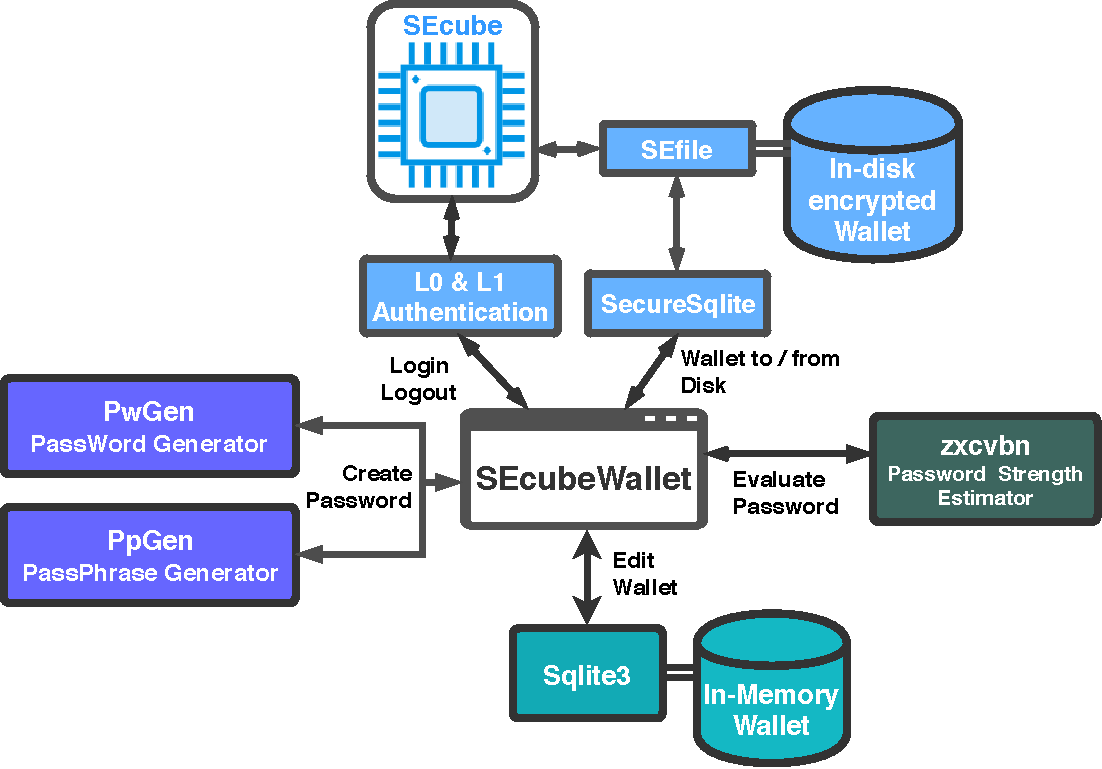
\includegraphics[width=\textwidth]{chapters/figures/development/BasicDesign.pdf}
	\caption{Basic Design: Used Libraries}
	\label{fig:BasicDesign}
\end{figure}

The following is a brief explanation of these Libraries and they usage. More details about each Library and why they were chosen are given in section \ref{sec:lib} and section \ref{sec:imp} deals with the actual implementation.

\subsection{L0 and L1 Authentication libraries}

When the user starts any application based on the SEcube™ platform, the first steps to perform are to open the communication with the device using Level0 functions from both host and device, and to authenticate the user by checking the login pin, using Level1 functions (again, from both sides). Figure \ref{fig:BasicDesign} depicts how the SEcubeWallet uses the authentication functions and they in turn communicate with the SEcube™ chip.

\subsection{secureSQLite3}
As explained before, Wallets are stored as SQLite DataBases. Fortunately, the SEcube™ SDK already provides a Level2 API for creating and managing encrypted SQLite DBs, called secureSQLite3. This API exploits the SEfile API to wrap some of the functions of the original SQLite3 library, avoiding OS calls.

secureSQLite allows to create/edit/save/open databases that when written to the disk are encrypted and can only be read when the SEcube™ is connected. Additionally, as it is implemented using wrappers, the developer only needs to include the source files in the project and can manage secureSQLite DB with the same functions used for regular SQLite DB. %TODO
\todo{cite secureSQLite}

Figure \ref{fig:BasicDesign} shows the SEcubeWallet application using secureSQLite to read/write the encrypted wallet stored in disk.

\subsection{SQLite3}
Because the use of secureSQLite involves a call to the SEcube™, a regular SQLite3 DB is also used, but unencrypted data is never saved to the disk. SQLite3 allows for the creation of an In-Memory DB, i.e. a DB whose content is always in the application's memory space and is therefore secured by the operating system. 

The In-memory DB is used for editing. When the user want to save the wallet, i.e. write it to the disk, the contents of the In-Memory DB are dumped to the encrypted secureSQLite DB. When the user opens a wallet from the disk, the reverse process occurs.

With the In-memory DB, unnecessary calls to the SEcube™ are avoided while maintaining the contents secured.

\subsection{Password Generator}
As the purpose of the application is to securely store passwords, said passwords should be as strong as possible. It does not make sense to protect a password that can be easily cracked by a hacker using brute force. That is why the application also includes a Password Generator.

PwGen \cite{pwgen} is an open source library that generates passwords, that can either be easy to remember, or completely random. Random passwords are more secure, but as the are difficult to remember, their use only makes sense when the user stores them in a wallet manager. Among other aspects, length and characters used (Numbers, Upper cases) can be configured too.

When the user is adding a new entry to a wallet, they can chose to enter a password or to automatically generate one.

\subsection{PassPhrase Generator}
In addition to the Password Generator PwGen, the user has the possibility to generate PassPhrases instead. PassPhrases are a popular alternative because they are easier to memorize and therefore can be longer, which in turns make them more secure. Further details about the usefulness of PassPhrases and how they compare against regular Passwords is given in section \ref{sec:zxcvbnth}.

Although the PassPhrase Generator is not a library per se, it was included in the diagram because of its close relation with the PwGen and zxcvbn \cite{zxgit} libraries. It was developed by the author, and it works by selecting random words out of dictionary files. 

The user can configure how many words each passphrase must have, the minimum length of said words, and which dictionary files to use, among other options.

\subsection{Strength Estimator}
To give the users feedback on how good the password they are about to store is, the application uses the open source project zxcvbn to give an estimation of the passwords entropy, and how long it would take for a hacker to break it. zxcvbn evaluates if the password is a common word, or a combination of them, a last name, a date, or letters close to each other in a keyboard (thus the name zxcvbn). With the estimator users are encouraged to create good passwords that are not necessarily completely random and difficult to remember, or annoying to type.

%\vspace{15pt} 
\vskip 25pt

To recap, these are the key aspects of the used libraries:

\begin{itemize}
\setlength\itemsep{0pt}

\item To start the connection with the SEcube™, the Level0 library is used
\item To authenticate the user, by checking if the entered login pin is the same as the pin stored in the SEcube™, the Level1 library is used.
\item An in-memory database is used for editing the wallet.
\item An encrypted in-disk data base is used for storing the wallet in disk.
\item The application includes a password generator with several options.
\item The application also includes a password strength estimator, so the user has an idea of how good their passwords are.

\end{itemize}

\section{Frameworks, Libraries and software tools} \label{sec:lib}

As explained in the previous section, the core of the design is the use of the SEcube™ chip to perform security operations in order to encrypt/decrypt some data stored in the host (PC). The requests to the chip are made from the Qt application developed in this work, which runs in the host. Said application exploits the existing C libraries SEfile and secureSQLite to ease the communication with the SEcube™. Additionally, the application also makes use of a random password generator PwGen and a strength estimator zxcvbn open libraries. 

In the following sections a review of the SEcube™ platform's hardware and software components is given. Then a brief explanation of the C++/Qt framework and why it was chosen. Finally the additional used libraries are presented.

\subsection{The SEcube™ framework}

``The SEcube™ (Secure Environment cube) Open Security Platform is an open source security oriented hardware and software platform, designed and constructed with ease of integration and service-orientation in mind. The hardware part of the platform was originally designed by Blu5 Group \cite{Blu5}, whereas the software libraries stem from a strong cooperation among international research institutions.'' \cite{GetStart}.

\vspace{5pt}

The main \textbf{hardware} products, explained in detail in the following sections, are:
\begin{itemize}
\setlength\itemsep{0pt}
\item The Chip, named SEcube™ Chip, or simply \textbf{SEcube™}
\item The Development Board, named \textbf{SEcube™ DevKit}
\item The USB Stick, named \textbf{USEcube Stick}.
\end{itemize}

The SEcube™ chip is the main hardware component, and both the devkit and USB Stick are designed around it.The Development Board provides several communication protocols as well as debugging capabilities. For the final product the board would be of course too inconvenient to carry, and instead the USEcube Stick is preferred.

\subsubsection{The SEcube™ Chip}

``The SEcube™ (Secure Environment cube) is a powerful chip which
integrates three key security elements in a single package. A fast
floating-point Cortex-M4 \textbf{CPU}, a high-performance \textbf{FPGA} and an
EAL5+ certified Security Controller (\textbf{Smart Card}).
The result of this innovative combination gives an extremely
versatile secure environment in a single SoC, in which developers
can rapidly implement complex applications and appliances.
... The SEcube™ is the ultimate solution for high-end design,
delivering integration of a flexible, configurable and certified
secure element.'' \cite{SEcubeDS}

We can then see the SEcube™ chip as a powerful device offering the flexibility of an \textsc{ARM} CPU, the speed of an FPGA and the reliable security of a certified Smart Card, all bounded together and easily integrated in any project thanks to the available communication protocols, among them USB, UART, Ethernet and JTAG. 

The chip includes a true random number generator which relies in 240 noise seeds, all physical and therefore unpredictable. This allows the creation of true random noise. Additionally the user can choose what type of noise they want to generate, for instance white or Fourier noise.

%TODO
\todo{talk more about cpu, low power modes...}

In figure \ref{fig:SEcubeBD} a simplified SEcube™ architecture is shown.

\begin{figure}[ht]
	\centering
	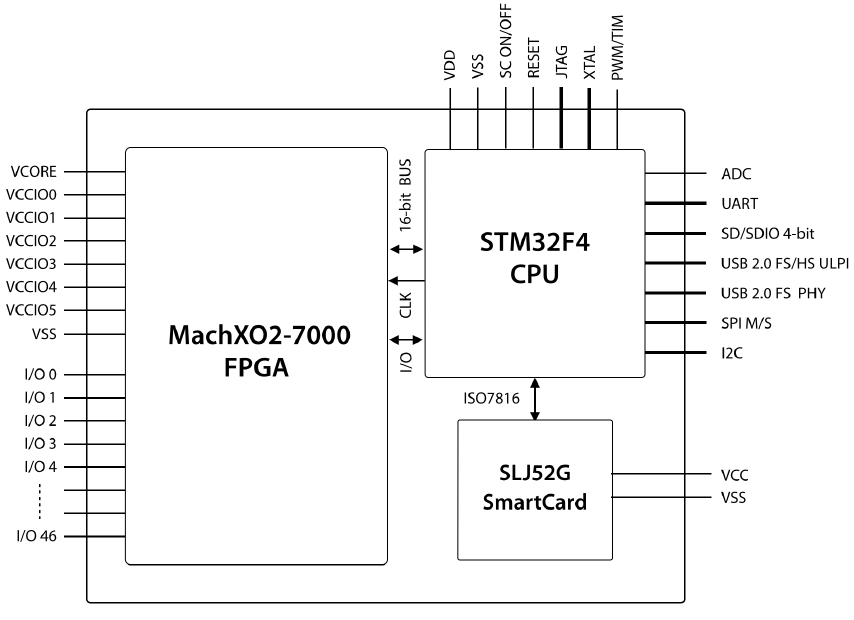
\includegraphics[width=\textwidth]{chapters/figures/development/SEcubeBlocks.png}
	\caption{SEcube™ Block Diagram}
	\label{fig:SEcubeBD}
\end{figure}


\subsubsection{Development board: The SEcube™ DevKit}

The development board integrates the SEcube™ chip with several peripherals that allow the user to easily communicate, program and debug. (Figure \ref{fig:devboard})

\begin{figure}[ht]
  \centering
  \subfloat[]{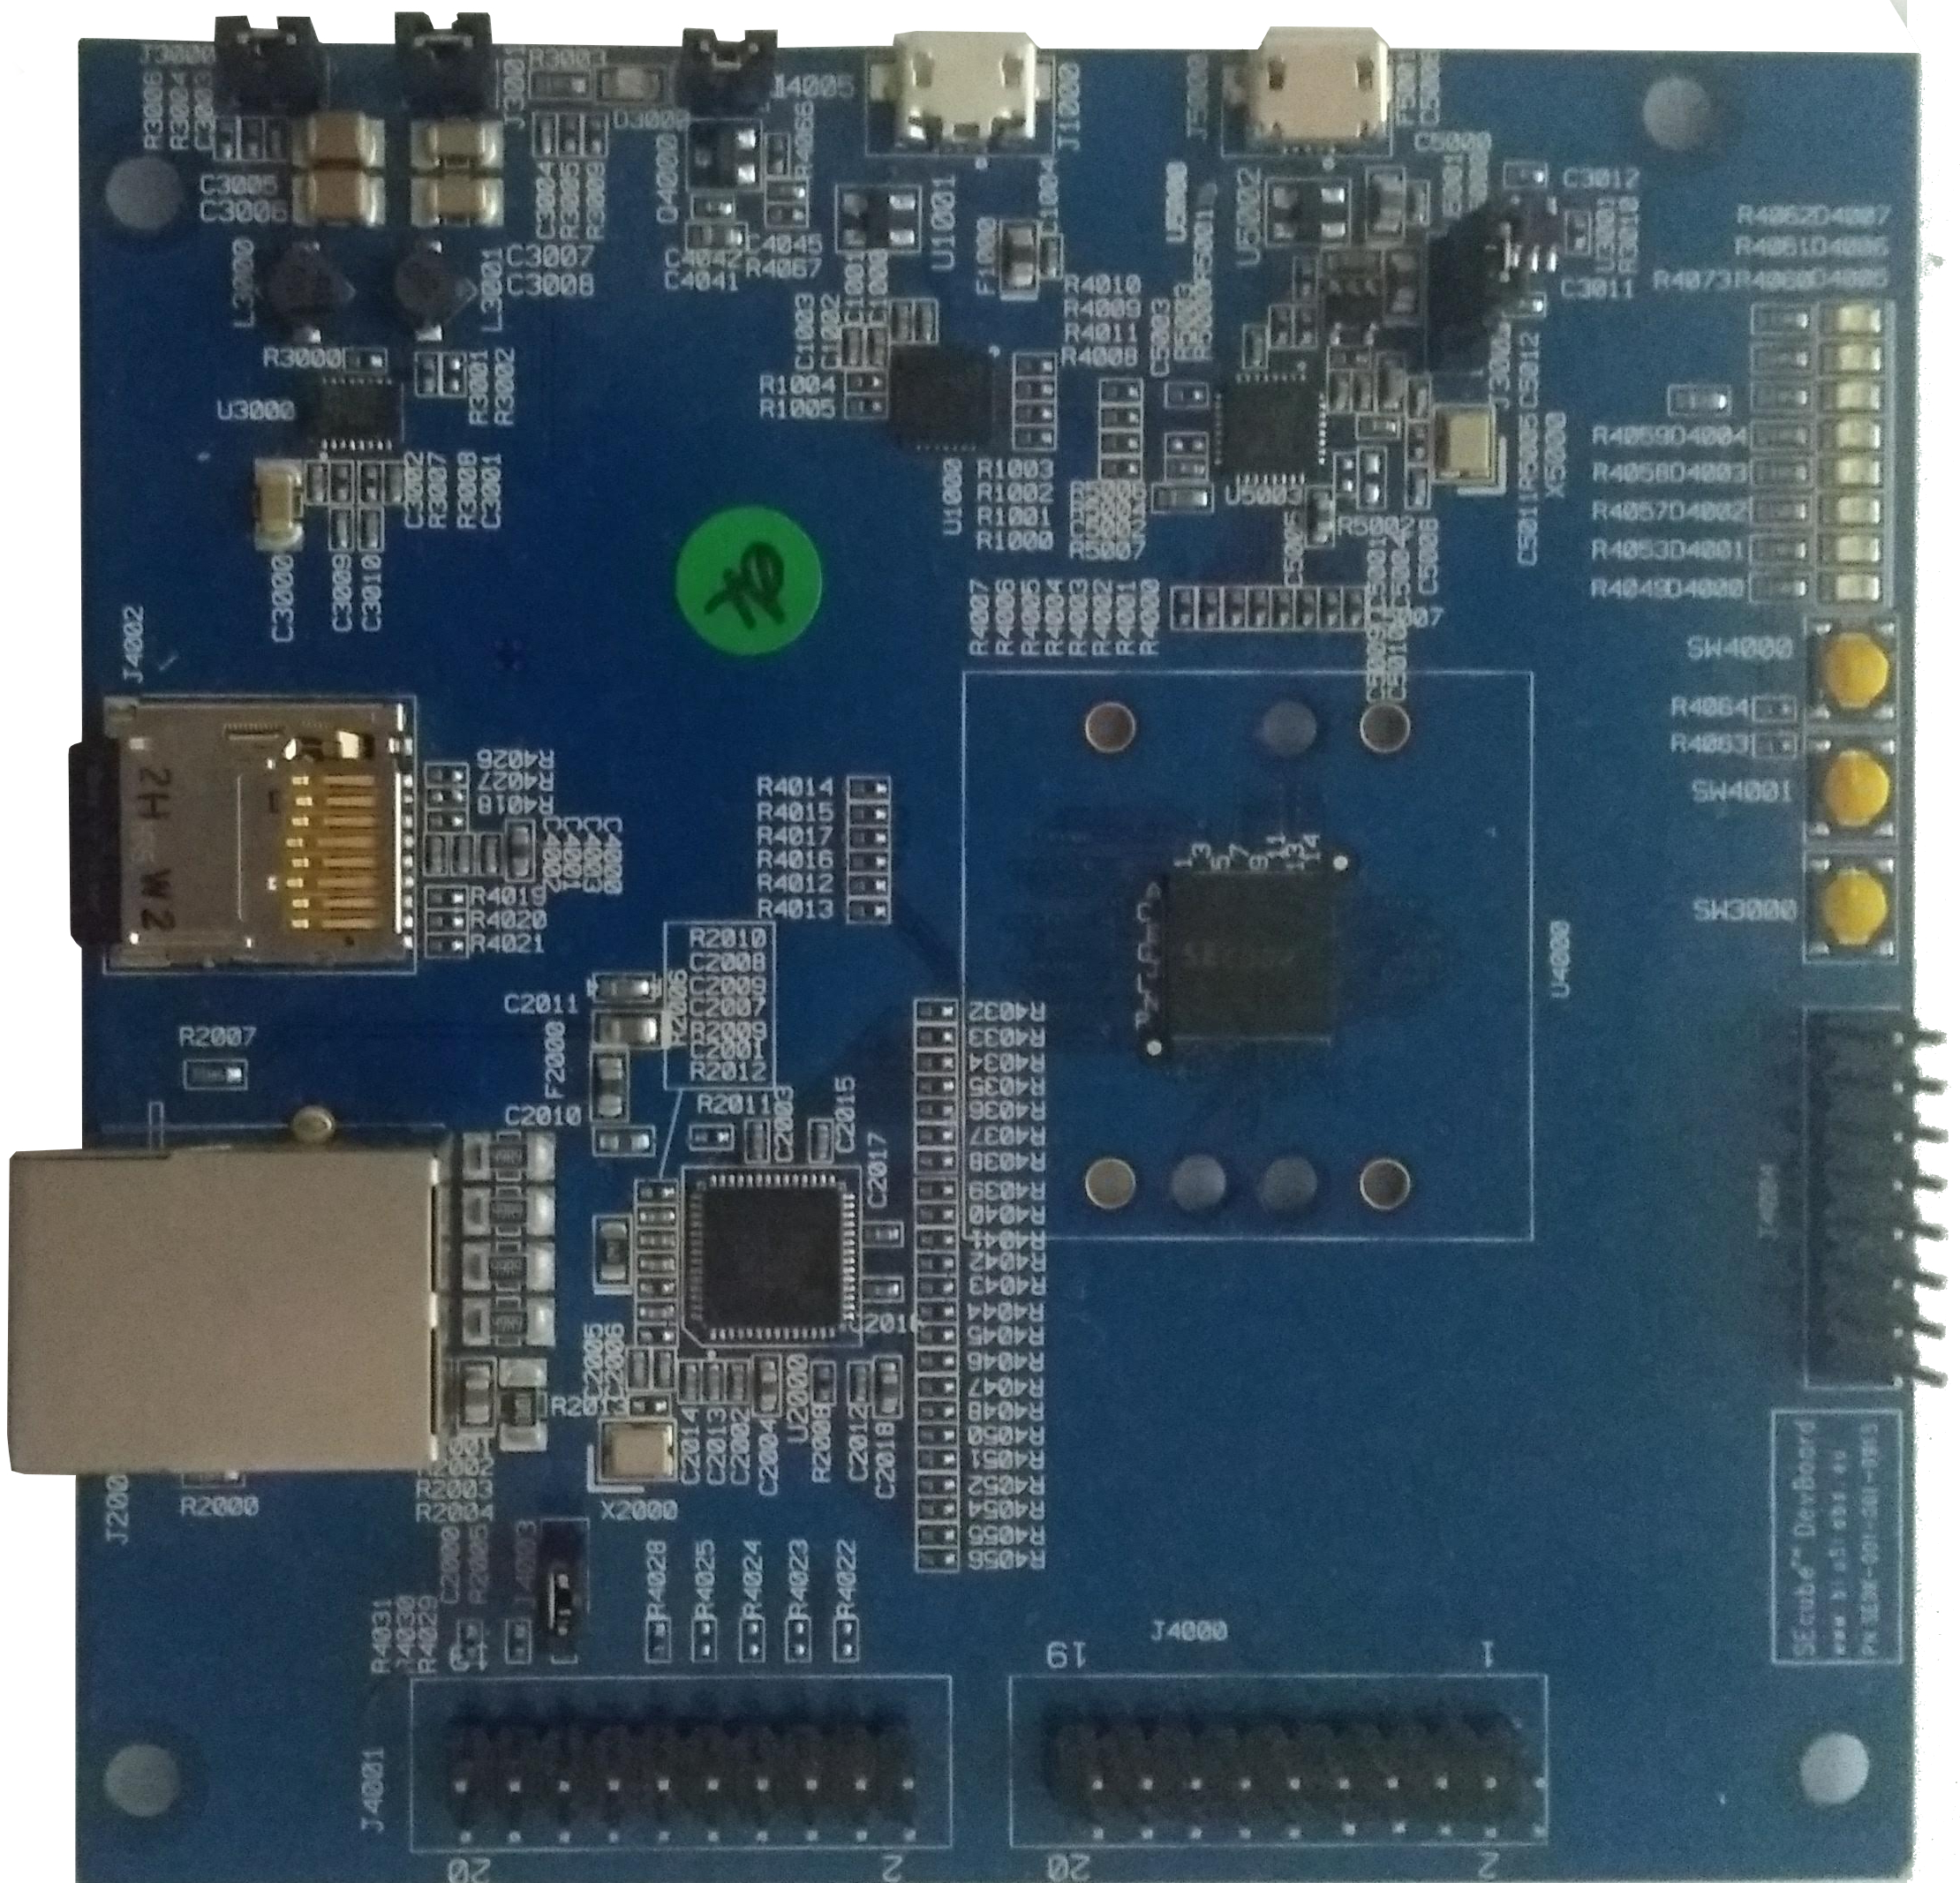
\includegraphics[width=0.485\textwidth]{chapters/figures/development/devboard.jpg}}
  \subfloat[]{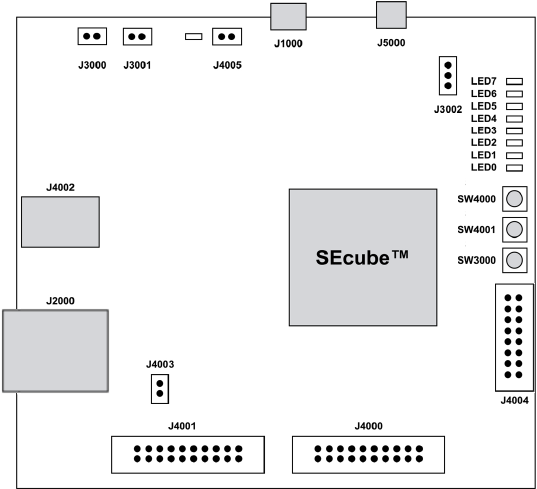
\includegraphics[width=0.515\textwidth]{chapters/figures/development/devboard_sch.png}}
  \caption{SEcube™ Devkit}
 \label{fig:devboard}
\end{figure}

The main peripherals in the SEcube™ devkit are:

\begin{itemize}
\setlength\itemsep{-3pt}
\item \textbf{J1000: }\tabto{2.3cm} USB 2.0 to UART 
\item \textbf{J2000: }\tabto{2.3cm} Ethernet 10/100 socket 
\item \textbf{J4000: }\tabto{2.3cm} SEcube™ embedded FPGA and CPU GPIOs
\item \textbf{J4001: }\tabto{2.3cm} SEcube™ embedded CPU JTAG
\item \textbf{J4002: }\tabto{2.3cm} microSD card 
\item \textbf{J4004: }\tabto{2.3cm} SEcube™ embedded FPGA and CPU GPIOs
\item \textbf{J5000: }\tabto{2.3cm} USB 2.0 High Speed 
\item \textbf{LEDx:  }\tabto{2.3cm} Leds 
\item \textbf{SWx00y:}\tabto{2.3cm} Switches 
\end{itemize}

\subsubsection{Final product: USEcube Stick}

For the final product, its is desired that the user carries all the SEcube™ functionalities in a small and convenient package, so they can encrypt/decrypt the passwords in any PC by just connecting the USEcube Stick and running the SEcubeWallet application.

The USEcube Stick is compatible with any Operating System and the SEcube™ functionalities are easily exposed to applications and services without installing any driver.

The USEcube offers only the strictly required components: The SEcube™ chip, a USB 2.0 High-Speed interface and an SDcard socket. See Figure \ref{fig:USEcube} for more details.


Since the USEcube Stick storage capability is based on a external microSD card, the security of the system is improved, as this allows to have a separation of encrypted data from the encryptor/decryptor. Additionally, both the size and the speed can be tuned per the user requirement and can be changed at any time, just replacing the microSD, without buying a new USEcube Stick.
The microSD card socket is embedded in the USB connector allowing to save space making the USEcube Stick very compact and, at the same time dust
and water-resistant.
Since the USEcube Stick is not provided with the JTAG interface, to inject the firmware previously developed and tested on the SEcube™ DevKit, all the devices come with an embedded secure boot loader.


\begin{figure}[ht]
  \centering
  \subfloat[]{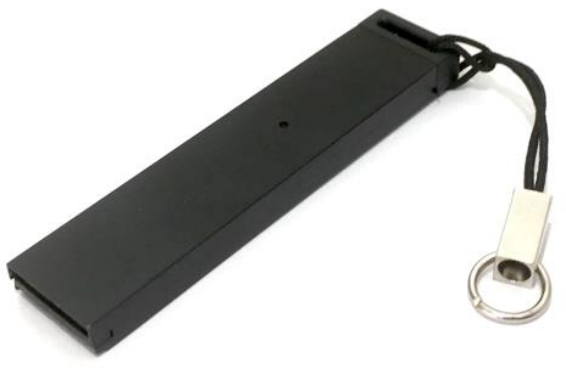
\includegraphics[width=0.485\textwidth]{chapters/figures/development/usb.png}}
  \subfloat[]{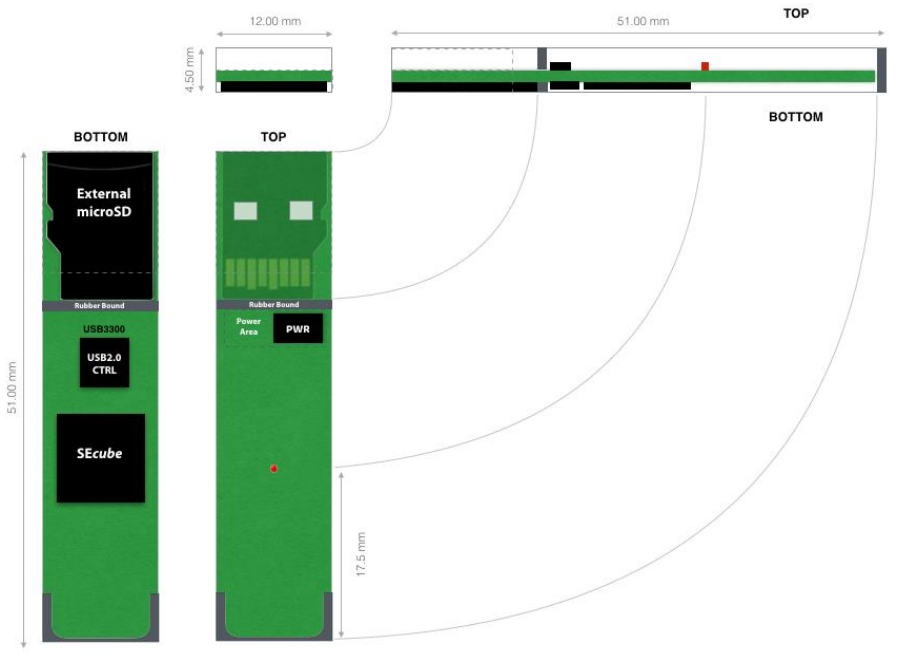
\includegraphics[width=0.515\textwidth]{chapters/figures/development/usb_sch.png}}
  \caption{USEcube Stick}
 \label{fig:USEcube}
\end{figure}


\subsubsection{L2 Security APIs}

``The software libraries and design environment allow developers who are not willing or able to produce the security APIs and protocols themselves to exploit the ready functions provided (currently as APIs and soon as services) within the SEcube™ platform and experience the platform as a high-security black box.'' \cite{L2UserMan}





``From the user/developer point of view, the APIs have been implemented targeting two
nested environments depending on where physically the code runs:
\begin{itemize}
\setlength\itemsep{1pt}
\item \textbf{Device-Side}, including the libraries of basic functionalities that are executed on the embedded processor of the SEcube™-based hardware device.
\item \textbf{Host-Side}, containing libraries of functions executed on the host PC and interface functions for calling services and processes residing on the embedded processor of the SEcube™ device.
\end{itemize} 

From the architectural point of view, the Host-Side Libraries have been implemented targeting 4 hierarchical abstraction levels, and namely:
\begin{itemize}
\setlength\itemsep{-3pt}
\item \textbf{Level 0:} Communication Protocol and Provisioning APIs
\item \textbf{Level 1:} Basic Security APIs (Level1 Host-Side – L1)
\item \textbf{Level 2:} Intermediate Security APIs (Level2 – L2)
\item \textbf{Level 3:} Advanced Security APIs (Level3 – L3).
\end{itemize}

At each level, each component represents a "service" for the upper level and relies on "services" provided by the next lower level, only.'' \cite{L2UserMan}

``Level L2 relies on L1 services to provide the APIs for implementing more abstract secure functionalities. Typical examples include APIs for the protection of data both at rest and in-motion, or negotiating parameters (e.g., keys, algorithms) for establishing secure sessions, without being forced to understand in details all the low-level hardware and security mechanisms.''\cite{L2UserMan}

L2 can be considered as the merge of two projects: \textbf{SEfile}, concerning data at rest, and \textbf{SElink}, concerning instead data at motion.

For our project we rely heavily on the development tools provided by the SEfile project, for the secure storage, usage and retrieve of data that requires a high degree of confidentiality, in our case, digital passwords.

\subsubsection{SEfile}

``SEfile targets any user that, by moving inside a secure environment, wants to perform basic operation on regular files. It must be pointed out that all encryption functionalities are demanded to the secure device in their entirety. In addition, SEfile does not expose to the host device details about what, or where it is reading/writing data: thus, the host OS, which might be untrusted, is totally unaware of what it is writing''. \cite{L2UserMan}.

\subsubsection{secureSQLite}

\subsection{SQLite3}

\subsection{Graphical User Interface: the Qt framework}
The application's graphical user interface was developed using the \textbf{Qt framework}, version 5.8.0. 

``Qt is a cross-platform application development framework for desktop, embedded and mobile. Supported Platforms include Linux, OS X, Windows, VxWorks, QNX, Android, iOS, BlackBerry, Sailfish OS and others. Qt is not a programming language on its own. It is a framework written in C++. A preprocessor, the MOC (Meta-Object Compiler), is used to extend the C++ language with features like signals and slots. Before the compilation step, the MOC parses the source files written in Qt-extended C++ and generates standard compliant C++ sources from them. Thus the framework itself and applications/libraries using it can be compiled by any standard compliant C++ compiler like Clang, GCC, ICC, MinGW and MSVC''.\cite{Qt}  


For writing, compiling and debugging source code, the IDE \textbf{Qt Creator}, version 4.2.1 was used.

``Qt Creator provides a cross-platform, complete integrated development environment (IDE) for application developers to create applications for multiple desktop, embedded, and mobile device platforms, such as Android and iOS. It is available for Linux, macOS and Windows operating systems''.\cite{QtC}.

\vspace{5pt}
The reasons behind the use of Qt are as follows:

\begin{itemize}
\setlength\itemsep{0pt}
\item Qt is a C++ library, and as such, allows for a seamless use of the C libraries SEfile and secureSQLite, which are the backbone of this project.

\item Qt is cross-platform, meaning the developed application can be compiled to work on any of the major OSes. In particular, the development was carried out an tested on a Linux machine, but the application should work with no problems in Windows and MacOS. 

\item Because of good designed and ready-to-use display items such as tables, menus and dialogues, it is possible to focus in writing the functional portions of the application without worrying too much about the GUI. And as it is open source, any Qt item can be modified and extended when it does not meet the expectations out of the box. In this project several display elements were improved, as will be seen in section \ref{sec:imp}.

\item Thanks to the multitude of functions dedicated to ease the use of C++ libraries and OS calls, one can be more productive, and the resulting code is more reliable. For instance, this project makes extensive use of such libraries, like QSqlDatabase, QString, QProcess, etc. Again, more details are given in section \ref{sec:imp}

\item Related works by research group \textsc{testgroup} from Politecnico di Torino using the SEcube™ framework, are written in Qt. Namely secureSQLiteBrowser and SEfile\_TXT, were used as base in the initial stages of development. This two projects can be found in the SEfileSDK available online \cite{SEcubeRes}.
%TODO
\todo{research group name  TESTGROUP?}

\item Qt is widely used, meaning it is possible to find tons of documentation, forums and additional libraries on the web. This also ensures the Qt framework will have continuous support from the developers and the community.

\end{itemize}



\subsection{PwGen: Pronounceable Password generator}

The most secure type of passwords are random ones. A random password sufficiently long is considered to be virtually unbreakable. But this rises two problems: First of all, humans are inherently bad at creating true random passwords. Second, a random password is not suited to be remembered or even used (as it probably is too annoying to type). These two reasons motivated the inclusion of a Password Generator.

pwgen is an open source program that generates human friendly passwords that are also secure. It is available in the official Linux repositories, and there is a Windows version as well, but in this work the source files where used.

``The pwgen program generates passwords which are designed to be easily memorized by humans, while being as secure as possible. Human-memorable passwords are never going to be as secure as completely completely random passwords. In particular, passwords generated by pwgen without the -s option should not be used in places where the password could be attacked via an off-line brute-force attack. On the other hand, completely randomly generated passwords have a tendency to be written down, and are subject to being compromised in that fashion'' \cite{pwgen}.

pwgen offers several options that can drastically change the type of generated password. Here is a list of the options available for users of SEcubeWallet:

\begin{itemize}
\setlength\itemsep{0pt}


\item \textbf{Length:} The desired length of the password. It is recommended to be at least 12 for non-random passwords and 8 for random ones.

\item \textbf{-0, no numerals:} 
Don't include numbers in the generated passwords. 

\item \textbf{-A, no capitalize:} 
Don't bother to include any capital letters in the generated passwords. 
    
\item \textbf{-B, ambiguous:}
Don't use characters that could be confused by the user when printed, such as 'l' and '1', or '0' or 'O'. This reduces the number of possible passwords significantly, and as such reduces the quality of the passwords. It may be useful for users who have bad vision, but in general use of this option is not recommended. 
    
\item \textbf{-c, capitalize:}
Include at least one capital letter in the password.

\item \textbf{-n, numerals:}
Include at least one number in the password.

\item \textbf{-s, secure:}
Generate completely random, hard-to-memorize passwords.

\item \textbf{-v, no vowels:}
Generate random passwords that do not contain vowels or numbers that might be mistaken for vowels. It provides less secure passwords to allow system administrators to not have to worry with random passwords accidentally contain offensive substrings. 

\item \textbf{-y, symbols:}
Include at least one special character in the password.
\end{itemize}

By default pwgen behaves as if the options \textbf{-nc} were used, that is, pronounceable passwords with at least 1 capital letter and 1 number.

The strongest passwords this program can generate are obtained with the options \textbf{-ys}, as it results in random passwords with special symbols. They are very hard to remember, and should only be used if the user is willing to open the SEcubeWallet application each time they need to use one of the password.


\subsection{zxcvbn: Password strength estimation} \label{sec:zxcvbnth}

An important feature to have in a password manager is the possibility to realistically estimate how strong a password is, i.e., how hard could it be for hackers to crack it, as there is no point in using the SEcube™ system to protect weak passwords, that could be easily guessed with brute force attacks. As it is out of the author expertise to write a reliable function to make this estimation, it was decided to use a trusted project developed during the dropbox hackweek event in 2012. The estimator called \textbf{zxcvbn} was originally written in JavaScript aiming for an easy integration with multiple web browsers and OS. Fortunately, the community ported the library to a wide variety of languages including Python, Ruby and C/C++. In this work the C++ implementation was used. The project is Open Source and available for free use on GitHub \cite{zxgit}.

zxcvbn is regarded by the community as one of the most reliable and mathematically advanced open source password estimators. In security forums and discussion it always pops out as an excellent tool, much better than other passwords estimators commonly used in web pages. In \cite{naked}, the author compares zxcvbn to other popular java meters and arrives to the conclusion that only zxcvbn is reliable enough to actually give an useful feedback.
In \cite{gen_est_eval}, the author makes an evaluation of several password generators and strength estimators. PwGen and zxcvbn, the two libraries used in this work, always give excellent results.

``For over 30 years, password requirements and feedback have largely remained a product of LUDS: counts of Lower- and Uppercase letters, Digits and Symbols. LUDS remains ubiquitous despite being a conclusively burdensome and ineffective security practice. zxcvbn is an alternative password strength estimator that is small, fast, and crucially no harder than LUDS to adopt. Using leaked passwords, we compare its estimations to the best of four modern guessing attacks and show it to be accurate and conservative at low magnitudes, suitable for mitigating online attacks. We find 1.5 MB of compressed storage is sufficient to accurately estimate the best-known guessing attacks up to 105 guesses, or 104 and 103 guesses, respectively, given 245 kB and 29 kB. zxcvbn can be adopted with 4 lines of code and downloaded in seconds. It runs in milliseconds and works as-is on web, iOS and Android''. \cite{zxpaper}

``People of course choose patterns — dictionary words, spatial patterns like \texttt{qwerty}, \texttt{asdf} or \texttt{zxcvbn}, repeats like \texttt{aaaaaaa}, sequences like \texttt{abcdef} or \texttt{654321}, or some combination of the above. For passwords with uppercase letters, odds are it’s the first letter that’s uppercase. Numbers and symbols are often predictable as well: \texttt{l33t} speak (3 for e, 0 for o, @ or 4 for a), years, dates, zip codes, and so on.
As a result, simplistic strength estimation gives bad advice. Without checking for common patterns, the practice of encouraging numbers and symbols means encouraging passwords that might only be slightly harder for a computer to crack, and yet frustratingly harder for a human to remember. xkcd nailed it''. (see figure \ref{fig:xkcd}). \cite{zxdropbox}

\begin{figure}[htb]
  \centering
  \captionsetup{justification=centering}
  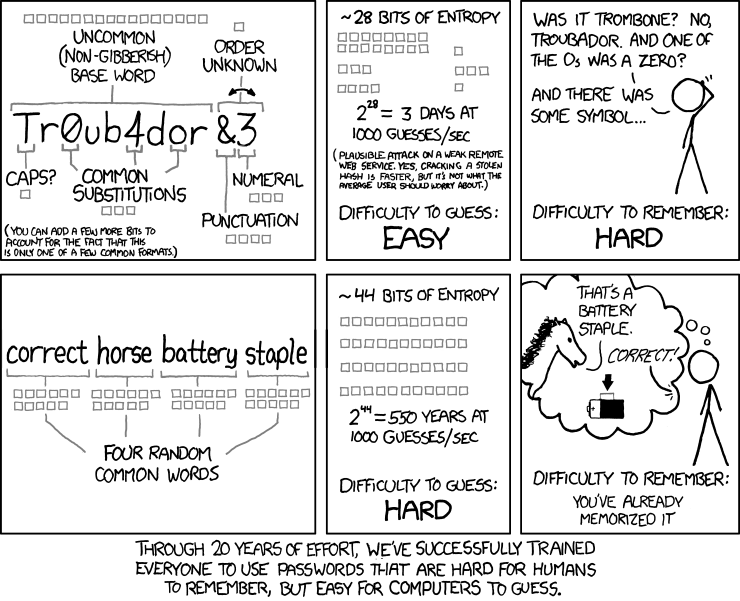
\includegraphics[width=\columnwidth]{chapters/figures/development/xkcd.png}
  \caption{Password strength, xkcd \cite{xkcd}}
  \label{fig:xkcd}
\end{figure}

To put it in other words, the authors of the project argue that a password like \texttt{correcthorsebatterystaple} (a nonsense English phrase) is more strong than a password like \texttt{Tr0ub4dour\&3}, even if the former does not have any upper cases or numbers, and the latter seems more complicated.

\begin{figure}[htb]
  \centering
  \captionsetup{justification=centering}
  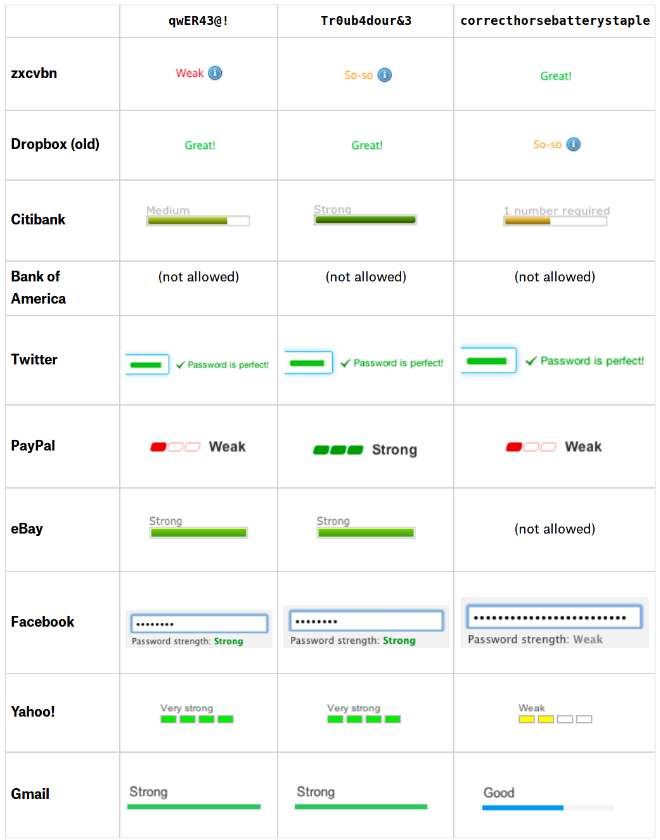
\includegraphics[width=\columnwidth]{chapters/figures/development/zxcvbn_comp.png}
  \caption{comparison between zxcvbn and popular websites' strength meters}
  \label{fig:tablez}
\end{figure}

The table in figure \ref{fig:tablez} (taken from \cite{zxdropbox}), show how zxcvbn is different from strength meters used in popular web services. (disclaimer: The data in the table is from 2012). From it we can learn:

\begin{enumerate}
\setlength\itemsep{-3pt}

\item Passwords like \texttt{\textbf{qwER43@!}}, which is a spatial password: it uses the keys \texttt{qwer4321}, with shift pressed for the keys \texttt{er} and \texttt{21} (the \texttt{@} symbol in the English keyboard is \texttt{shift+2}), is not considered week by most of the meters, but it should. It is probably due to the fact that it includes a combination of numbers and symbols that makes it look strong, but in reality, because of keyboard spatiality, is not.

\item Passwords like \texttt{\textbf{Tr0ub4dour\&3}}, which is generated by replacing some of Troubadour letters with numbers, and adding two more characters, is regarded as a very strong password for all of the meters except zxcvbn. Even if the base word is uncommon, and it has some variations, it is not long enough to be considered so strong.
\item A password like \texttt{\textbf{correcthorsebatterystaple}} is not considered strong by most of the meters except zxcvbn, and it is not even allowed in some cases because it lacks numbers, Upper-cases or symbols.
\end{enumerate}

The superiority of zxcvbn over the other meters in the table may seem like cherry picking, but the way zxcvbn is constructed explains these differences.

\subsubsection*{Matching}

Enumerates all the (possibly overlapping) patterns it can detect. Currently zxcvbn matches against:

\begin{itemize}
\setlength\itemsep{-3pt}


\item \textbf{Dictionaries:} Common words the user is likely to use as password. Multiple dictionaries, in a simple .txt format can be used. In this work, we present a few: English words, Italian words, names and surnames, Burnett’s 10,000 common passwords, words from tv and films. The match has an associated frequency rank, where words like the and good have low rank, and words like photojournalist and maelstrom have high rank. This lets zxcvbn scale the calculation to an appropriate dictionary size on the fly, because if a password contains only common words, a cracker can succeed with a smaller dictionary. For all dictionaries, match recognizes uppercasing and common \texttt{l33t} substitutions.

\item \textbf{Spatial keyboard patterns:} Some users are likely to choose passwords based on spatial pattern. For instance a user could choose the first row of letters from right to left: \texttt{poiuytrewq} as they password. \textsc{qwerty} keyboard, Dvorak keyboard, and keypad are considered.

\item \textbf{Repeats}: Users are also prone to use repetition of characters, like \texttt{rrrr}. 

\item \textbf{sequences}: Numeric or alphabetic sequences like \texttt{123} or \texttt{fedcba}

\item \textbf{years and dates}: The year or full date of a special event, like anniversary or birthday. Years from 1900 to 2019 are considered and dates in different formats. (3-13-1997, 13.3.1997, 1331997). 

\end{itemize}

\subsubsection*{Entropy calculation of a single pattern}
Depending on the type of matching, the entropy calculation is done differently, but for all the cases the idea is the same: How many different cases a hacker would have to try before guessing the pattern? For example, for the repeat case, if the user chooses \texttt{zzzzz}, as it is repeated five times, and if we assume the hacker starts by the letter a, then the number of cases would be $ N = 26 \times 5 = 130 $. (The sequence the hacker would try is: \texttt{a, b, c, d...,z, aa, bb, cc,...,...,zzzz, aaaaa, bbbbb,....zzzzz}).


As the number of possible cases can be pretty large, the entropy is not given as a raw value but as $e = log_{2}(N)$, known as the entropy bits, and in some cases as $f = log_{10}(N)$, known as the log entropy. In the example, entropy bits: $e = log_{2}(130) = 7 bits$.

The entropy bits and log entropy are related by:
\[N = 2^{e} = 10^{f}\]
\[f = e \times log_{10}(2)\]
\[e = f \times log_{2}(10)\]


\subsubsection*{Minimum entropy search of whole password}

``Given the full set of possibly overlapping matches, the algorithm finds the simplest (lowest entropy) non-overlapping sequence. For example, if the password is damnation, that could be analysed as two words, dam and nation, or as one. It’s important that it be analysed as one, because an attacker trying dictionary words will crack it as one word long before two.

zxcvbn calculates a password’s entropy to be the sum of its constituent patterns. Any gaps between matched patterns are treated as brute-force "patterns" that also contribute to the total entropy. That a password’s entropy is the sum of its parts is a big assumption. However, it’s a conservative assumption. By disregarding the "configuration entropy" — the entropy from the number and arrangement of the pieces — zxcvbn is purposely underestimating, by giving a password’s structure away for free: It assumes attackers already know the structure (for example, surname-bruteforce-keypad), and from there, it calculates how many guesses they’d need to iterate through.''\cite{zxdropbox}

\subsubsection*{From entropy bits to rank and estimated crack time} \label{sec:zxLevels}

To estimate the cracking time, it is necessary to make some assumptions about what kind of attack will be subjected the user. zxcvbn considers four possible scenarios according to the number of attempts/time the hacker can do:

\begin{enumerate}
\setlength\itemsep{-3pt}


\item \textbf{Online throttling (100 per hour):} Online attack on a service that ratelimits password authentication  attempts.
  
\item \textbf{Online no throttling (10 per second): }Online attack on a service that does not ratelimit or where an attacker has outsmarted ratelimiting.

\item \textbf{Offline slow hashing (1e4 per second): }Offline attack. assumes multiple attackers, proper user-unique salting, and a slow hash function with moderate work factor, such as bcrypt, scrypt, PBKDF2.

\item \textbf{Offline fast hashing (1e10 per second): }Offline attack with user unique salting but a fast hash function like SHA1, SHA256 or MD5. A wide range of reasonable numbers anywhere from one billion to one trillion guesses per second, depending on number of cores and machines. Ballparking at 10B per sec.

\end{enumerate}

%  0 # . (guesses < 10^3)
%
%  1 # very guessable: protection from throttled online attacks. (guesses < 10^6)
%
%  2 # somewhat guessable: protection from unthrottled online attacks. (guesses < 10^8)
%
%  3 # safely unguessable: moderate protection from offline slow-hash scenario. (guesses < 10^10)
%
%  4 # very unguessable: strong protection from offline slow-hash scenario. (guesses >= 10^10)

zxcvbn then ranks a password with a security level from 0 to 4 according to its entropy value:
\begin{itemize}
\setlength\itemsep{-3pt}

\item \textbf{Level0 if ($N<10^{3}$):} Too guessable, risky password
\item \textbf{Level1 if ($N<10^{6}$):} Very guessable, protection from throttled online attacks.
\item \textbf{Level2 if ($N<10^{8}$):} Somewhat guessable, protection from unthrottled online attacks.
\item \textbf{Level3 if ($N<10^{10}$):} Safely unguessable, moderate protection from offline slow-hash scenario.
\item \textbf{Level4 if ($N>10^{10}$):} Very unguessable: strong protection from offline slow-hash scenario

\end{itemize}
Where N is the number of possibilities a hacker would have to try for crack the password. So for instance, if the password is level 2, it could be cracked in around $10^{8}$ guesses.

For Level0 the above rule in terms of the entropy bits is $e<log_{2}(10^{3})$.
In terms of the log entropy bits, it simply is $f<3$.

The level and estimated crack time for each type of attack is presented to the user. With this information, the user will, hopefully, choose a Level4 password. Additionally, the user also receives  feedback about how the password was cracked, so they know how to improve it.

\subsection{PassPhrase Generator}

From the previous two sections there seems to be a disagreement on what a good password looks like. PwGen can generate totally random passwords or pseudo-random pronounceable passwords, but even the later go against what zxcvbn proposes: PassPhrases that are very easy to remember, but long enough to give excellent entropy results. To fill this gap, a PassPhrase generator that gives results along the lines of \texttt{CorrectHorseBatteryStaple} is used.

The PassPhrase generator developed by the author works by randomly picking out words from dictionary files. The user can tune the PassPhrase generation as follows:

\begin{itemize}
\setlength\itemsep{-3pt}

\item \textbf{Dictionaries: }The user must select appropriate dictionaries, containing a sufficiently large number of lines (larger than 10000) to ensure the picked words are really random. The English and Italian dictionaries used by zxcvbn are a good example. The user can work with as many dictionaries as desired, an the format must be one word per line. Only the first word of each line is counted, as everything after a space is trimmed.

\item \textbf{Number of words: }The user can configure the number of words the generated PassPhrases are composed of. The recommended size is four, but it can be as long as the user wants.

\item \textbf{Minimum Length of Words: }With this option is possible to select only random words whose length is higher than a certain value. This is to make sure the resulting PassPhrase is too short and therefore too insecure. The drawback here is that the higher the selected threshold, the fewer the available words in the dictionaries.

\item \textbf{Only use infrequent words: }If the dictionaries follow the same format as those used for zxcvbn, that is, the words are ordered by frequency, having the most uncommon words in the lower part of the dictionary, the user can then ask to generate PassPhrases containing only unusual words. The drawback here is, again, fewer words to choose from. The percentage of words that are used is configurable.

\item \textbf{Capitalize first letter: }To make the PassPhrases more readable, the first letter of each word can be capitalized.
\end{itemize}



\subsection{Device side development: Eclipse}

\section{Implementation} \label{sec:imp}

%TODO
\todo{subdirs structue in qt project}

In the following sections each of the elements and functionalities of the application will be explained, how they were implemented, some interesting pieces of code and examples of use.

\subsection{User authentication}

When the user starts the application, the first window to appear is the Login Dialogue, shown in figure \ref{fig:logina}. In it the user is asked to enter the login pin and by clicking accept the Challenge-Based Authentication process between the SEcubeWallet application and the SEcube™ chip starts. If the authentication fails because the entered pin is wrong, the message in \ref{fig:loginb} is shown. If it fails because there was already an opened session, the confirmation dialogue shown in \ref{fig:loginc} appears. If the authentication is completed successfully the user is granted access to the main window.

\begin{figure}[ht]
  \centering
  \subfloat[Login Dialogue\label{fig:logina}]
  {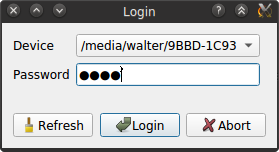
\includegraphics[width=0.3\linewidth]{chapters/figures/development/login.png}}
  {}
  \subfloat[Wrong Password\label{fig:loginb}]
  {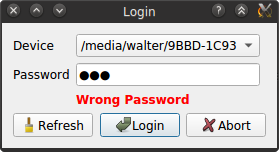
\includegraphics[width=0.3\textwidth]{chapters/figures/development/loginWrong.png}}
  {}
  \subfloat[Already an open session\label{fig:loginc}]
  {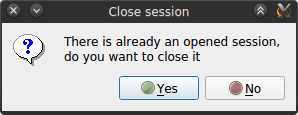
\includegraphics[width=0.3\textwidth]{chapters/figures/development/loginOpen.png}}
  \caption{Login Dialogue and possible outcomes}
 \label{fig:login}
\end{figure}

The authentication process begins with the discovery of SEcube™ devices connected to the PC. This is achieved using Level0 APIs as seen in the listing \ref{lis:dis}. Each discovered device is added to the \texttt{QComboBox} displayed in the login dialogue and to a \texttt{QList}.

\begin{lstlisting}[style=customc, float=htb, caption={Connected Devices discovery}, label = {lis:dis}]
//// *** variables declaration ***
se3_disco_it it;
QList<se3_disco_it> device_found;
QComboBox* chooseDevice;
bool found = true;

//*** Refresh button slot *****
L0_discover_init(&it); //initialize iterator
while((found = L0_discover_next(&it))){ //move to next device
  chooseDevice->addItem(QString::fromLocal8Bit(
    it.device_info.path, -1)); //add to GUI
  device_found.push_back(it); //add to QList
}
\end{lstlisting}

The user then selects one of the discovered devices using the \texttt{QComboBox}, enters their login pin and clicks accept. This triggers the listing \ref{lis:login}. The first step is to open the device communication using the Level0 function \texttt{L0\_open}. Then \texttt{L1\_login} starts the actual challenged based authentication using the login pin entered by the user. Using this type of authentication ensures the login pin is never communicated between the devices and stolen with a physical attack on the USB cable. Rather, a random number is generated in the host and transmitted to the device. The login pin is then used in both the host and the device to encrypt this random number using a \texttt{pbkdf2} function. The resulting key on the device is sent to the host, who compares it with its own key. If they are the same it means the login pin entered by the user is equal to the login pin stored in the device, and the only information transmitted are random numbers that an attacker cannot understand. (The actual authentication procedure implemented is a little bit more complex, but is based on the same idea described here).
%TODO
\todo{explain better the challenge based}

\begin{lstlisting}[style=customc, float=htb, caption={Open device and try to login}, label = {lis:login}]
// *** variables declaration ***
//use selected index at QComboBox to retrieve 'it' from QList.
int device_index = chooseDevice->currentIndex();
se3_disco_it it = device_found.at(device_index);

se3_session s; 
se3_device dev;
int ret;
bool logout = false; //if true, L1_login logs out first

//*** Accept button slot *****
if(!dev.opened) // open communication with device
  if((L0_open(&dev, &(it.device_info), SE3_TIMEOUT))!= SE3_OK)
    exit(1); //error

ret = L1_login(&s, &dev, pin, SE3_ACCESS_USER, logout); //login

if (ret != SE3_OK){    //error at login
  if (ret == SE3_ERR_PIN) //The password is wrong
    show_wrong_pass_messsage;
    
  else if (ret == SE3_ERR_OPENED){
    // there is already an opened session, ask user if he wants to close it
    if(confirmation_dialog_reply == Yes){ 
      logout = true; 
      call_this_function_again;
      //next time L1_login will close the existing session
    }
  }else            
    exit(1);//other error
}else
  accept();//All ok, go to main window
\end{lstlisting}

After both device and host have the same key, it is used to encrypt the communication channel. A token is generated in the device and transmitted on the encrypted channel to the host. This token is a random number, and is used from that point on to validate any communication between host and device. The SEcubeChip does not accept any command from the host if the token it sends is not the correct one. The only command accepted without a token is off course, login. In the logout procedure, this token is cleared (set to zeros), so a login later on is possible.

One problem found during the development of the application is the followin: If after login in, the SEcubeWallet application crashes, the logout command, that is usually issued when closing, is never executed, and the device remains with an active token value. Therefore, when the user launches the application again, the login will fail, because the device expects a token value from the host. To solve this issue a few options were considered:

\begin{itemize}
\setlength\itemsep{-3pt}

\item Make sure the application never crashes. Because software applications are rarely completely bug-free, and even if they are, an external problem like a bug in the OS can make them crash, this option is not feasible. 
\item Make sure the logout command is issued even in the case the application crashes. This option sounded promising, and a two-process idea was even developed. Process 1 is only in charge of calling Process 2, in which the actual application was executed. if Process 2 crashes, Process 1 remains alive and performs the logout procedure. To make this work, shared memory was used to communicate the session variable (were the token is stored), so both processes could send commands to the device. The idea was latter on dropped because of two main reasons: First of all, it did not solve the case were the problem is external (OS bug), secondly, it was too complicated because of the sharing memory mechanism (The session variable is a fairly complex structure, with a lot of pointers), and because the token was being shared by two processes, this could open another possibility of attacks.
\item As the two previous ideas failed, it was decided that a small modification to the login behaviour on the SEcube™ firmware was necessary. The modification consist on letting the login function clear the token field if necessary. This does not compromise the security of the system because access to the chip is only granted if the login pin entered by the user is the right one. One concern that may rise is that, while an application is using the SEcube™, another one could close the session by issuing a Login command, but this is not possible because the \texttt{L0\_open} function only allows one process to communicate with the chip at a time, using a file locker in the .se3magic
file saved in the SEcube™ SDcard.
\end{itemize} 

The new behaviour is implemented in listings \ref{lis:se3cmd1}.
If after a crash the session in the SEcube™ remains open, and the host tries to login again, the SEcube™ returns the new error code \texttt{SE3\_ERR\_OPENED}. The host then can decide if it wants to force the SEcube™ to close the opened session so it can login, with the new command \texttt{SE3\_CMD1\_LOGOUT\_FORCED}, which forces a logout without checking the token. After this command the host can login as usual. This steps are included in the host side \texttt{L1\_login} function, which now has an additional parameter to control whether to force a logout or not. This parameter is the one used in listings \ref{lis:login}, set to true when the user clicks \textsc{yes} in the confirmation dialogue asking whether or not to close the previous session.

\begin{lstlisting}[style=customc, float=htb, caption={Modification in SEcubeFirmware, file se3\_cmd1.c}, label = {lis:se3cmd1}]
if (se3c1.login.y) { // if there is already an opened session
  if (memcmp(se3c1.login.token, req_params.token, SE3_L1_TOKEN_SIZE)) { //and token mismatch
    if (req_params.cmd==SE3_CMD1_CHALLENGE)//someone (maybe same user after a crash) trying to login.
      return SE3_ERR_OPENED;//notify host there is already an opened session, if host wants to continue, it will call SE3_CMD1_LOGOUT_FORCED
    else if (req_params.cmd==SE3_CMD1_LOGOUT_FORCED)//if the user agreed to close the existing session by forcing a logout
      req_params.cmd=SE3_CMD1_LOGOUT;//call logout as usual  
    else
      return SE3_ERR_ACCESS;
  }
}
\end{lstlisting}




\subsection{Main Window}

The SEcubeWallet GUI's main window developed using Qt is shown in figure \ref{fig:mainWindow}.

\begin{figure}[htb]
  \centering
  \captionsetup{justification=centering}
  \centerline{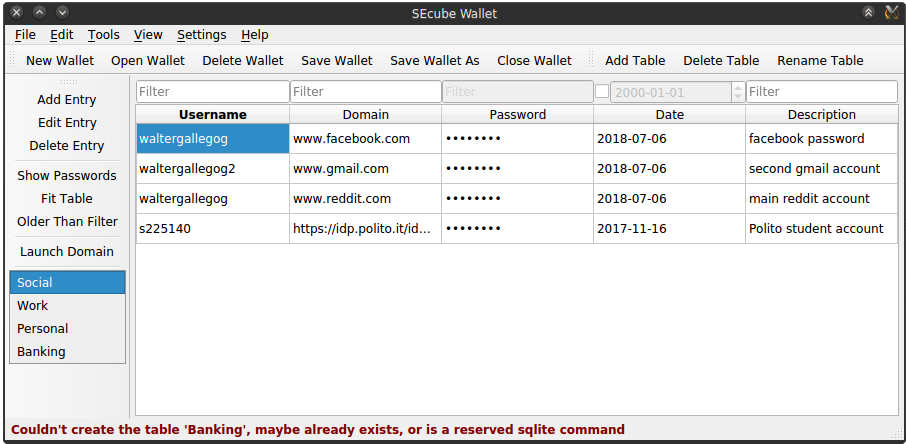
\includegraphics[width=1\columnwidth]{chapters/figures/development/mainWindow.png}}
  \caption{SEcubeWallet main window}
  \label{fig:mainWindow}
\end{figure}

The main window is composed of the following elements:

\begin{itemize}
\setlength\itemsep{-3pt}

\item \textbf{Table View:} Used for displaying the wallet entries. It resizes smoothly with the window, can be ordered by any of the columns, and the passwords are hidden by default but can be shown if the user wants to.
\item \textbf{Filters:} The user can search in each of the table's columns using filters. These filters are implemented inside a separate container, but they resize together with the table.
\item \textbf{Entries Tool Bar:} It is positioned to the left of the table. It has the actions: add/edit/delete entries, show passwords, fit table, change date filter, launch domain and select table.
\item \textbf{Tables Tool Bar:} It is positioned to the top right of the table. It has the actions: add/rename/delete table.
\item \textbf{Wallets Tool Bar:} It is positioned to the top left of the table. It has the actions: new/open/delete/save/save as/close Wallet. 
All of the above Tool Bars are movable.
\item \textbf{Menu Bar:} It is positioned at the top of the window. It contains all the previous actions, plus preferences and help.
\item \textbf{Status Bar:} Positioned at the bottom of the window, it is used to display some success/error messages to the user and the current wallet name.
\end{itemize}

\subsection{Wallet actions}

The actions regarding wallets: New, Save, Save As, Open, Close and Delete are explained in detail in the following.

\subsubsection*{New Wallet action}

When the user triggers the the \texttt{New\_Wallet} action, the first step to execute is to check if there is another wallet opened and if it has unsaved changes. If, so the confirmation dialogue in figure \ref{fig:confSave} is shown, so the user can decide whether to save the changes, discard them, or cancel the creation of a new wallet.
\begin{figure}[htb]
  \centering
  \captionsetup{justification=centering}
  \centerline{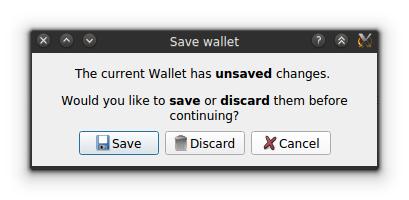
\includegraphics[width=0.6\columnwidth]{chapters/figures/development/confSave.png}}
  \caption{Save Confirmation dialogue}
  \label{fig:confSave}
\end{figure}

In case the user clicks \texttt{Save}, the \texttt{Save\_Wallet} action is triggered before continuing. \texttt{Discard} continues without saving, and \texttt{Cancel} returns without doing anything.

If the process continues, the next step is to close any previous in-memory database handlers, save the \texttt{table\_view} geometry (if any), and open a new in-memory database using the Qt class \texttt{QSqlDatabase}, as seen in listings \ref{lis:newDB}.

\begin{lstlisting}[style=customc, float=htb, caption={New in memory database}, label = {lis:newDB}]
QSqlDatabase dbMem; //The database handler, declared in header 

//Check if SQLite is installed on OS
if(!(QSqlDatabase::isDriverAvailable("QSQLITE")))
  exit (1); //the application does not work without SQLite

if (dbMem.isOpen()){ 
  save_table_geometry;
  dbMem.close();//close any prev. opened database
}

dbMem = QSqlDatabase::addDatabase("QSQLITE");
dbMem.setDatabaseName(":memory:"); // in-memory database
if(!dbMem.open()){
  return;//Error opening, do nothing
}
\end{lstlisting}

As explained before the in-memory data base is used for editing. It has the advantage of being fast because there is no access to the hard disk, and secure, because all the data is in the application memory space, and therefore is protected by the OS.

The last step is to update the GUI state, by enabling some action like \texttt{Add\_Table} and \texttt{Save\_Wallet}, and disabling others, like \texttt{Delete\_Table} and \texttt{Rename\_Table}.

\subsubsection*{Save Wallet action} \label{sec:savewalletaction}
To write the wallet contents to the disk, it is necessary to have a filename, so the first step is to check if the user already entered one (from previous saves). If not, with the dialogues in figure \ref{fig:saveWallet} the user can choose the directory and the filename to save.

\begin{figure}[ht]
  \centering
  \subfloat[User can enter a New name. Current wallets are displayed\label{fig:saveWalleta}]{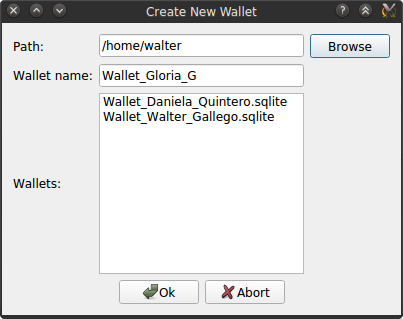
\includegraphics[width=0.48\textwidth]{chapters/figures/development/saveWallet.png}}
  {}
  \subfloat[if \texttt{Browse} is clicked a \texttt{QFileDialog} is launched\label{}]{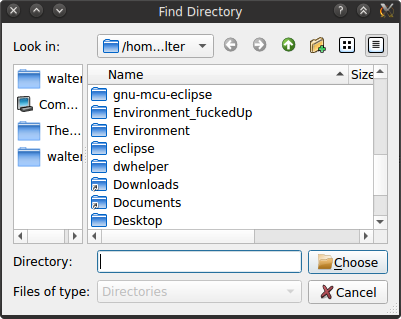
\includegraphics[width=0.48\textwidth]{chapters/figures/development/directories.png}}
  \caption{Save Wallet dialogues}
 \label{fig:saveWallet}
\end{figure}

The need for two dialogues instead of a regular file browser comes from the fact that the chosen filename will not be readable from the OS, since \texttt{SEfile} also encrypts it. Similarly, wallets already saved in the directory cannot be displayed with a regular file browser, so it is necessary to use the \texttt{SEfile} function \texttt{secure\_ls} and display its output in the list seen in figure \ref{fig:saveWalleta}. The declaration of this function is in listings \ref{lis:securels}. To chose the working directory, it is enough to use the \texttt{QFileDialog} class. If the user wishes they chose an existing filename and can overwrite the correspondent wallet.

\begin{lstlisting}[style=customc, float=htb, caption={\texttt{secure\_ls} declaration}, label = {lis:securels}]
 /* This function identifies which encrypted files and encrypted directories are present in the directory pointed by path and writes them in list. It only recognizes the ones encrypted with the current environmental parameters.*/
 
uint16_t secure_ls(    //returns 0 in case of success
  char *path,          //[in]Path to the directory to browse
  char *list,          //[out]Allocated array to store filenames
  uint32_t *list_length//[out]Num of char written in list
);
\end{lstlisting}


After having a filename the next step is to read all of the tables in the current in-memory database, row by row. For each row a \texttt{SQLite} statement of the form \texttt{INSERT INTO table VALUES(user, dom, pass, date, desc)} is created. All of them are merge into a single statement which is executed into the secured in-disk database. This ensures only one access to the SEcube™ and disk. This process is somewhat slow and the GUI is disabled while it is performed. A simplified version of the code is shown in listing \ref{lis:save} 

\begin{lstlisting}[style=customc, float=htb, caption={simplified Save process}, label = {lis:save}, escapechar=¬]
sqlite3 *dbSec;    //Secure database declaration, in header
QSqlDatabase dbMem;//The database handler, declared in header 
QSqlQuery query;   //To exec SQLite statements, dec. in header

//Create SQLite DB, with filename specified by user If SEcube is connected, the resulting file is encry.
sqlite3_open_v2 (fileName.toUtf8(),   
                &dbSec, 
                SQLITE_OPEN_READWRITE | SQLITE_OPEN_CREATE , 
                NULL) 
                
QString finalSql; //To Merge all the SQLite statements.
static const QString insert = 
  QStringLiteral("INSERT INTO '%1' VALUES(%2);"); //statement
  
dbMem.tables(QSql::Tables); //list of the tables in in-memory DB
tables.prepend("NoEmpty");  //Workaround: prepend Empty table   ¬\label{line:empty}¬
foreach (const QString table, tables) { // loop all the tables
   QString sql= "create table '"+table+//Create table statement 
                "'(id integer primary key, "
                "Username TEXT, "
                "Domain TEXT, "
                "Password TEXT, "
                "Date TEXT, "
                "Description TEXT );" ; 
  sqlite3_exec(dbSec, sql.toUtf8(), NULL, 0, &zErrMsg);// exec
  
  if (table=="NoEmpty"){//just an empty table
    set_values_to_empty;
    finalSql += insert.arg(table).arg(values.join(", "));
  }else{
    query.prepare(QString("SELECT * FROM [%1]").arg(table));
    query.exec()
    while (query.next()){ //row by row
      values = query_read_row();
      finalSql += insert.arg(table).arg(values.join(", "));
    }
}
//single write into secure database, fill the tables
sqlite3_exec(dbSec, finalSql.toUtf8(), NULL, 0, &zErrMsg);
\end{lstlisting}

One problem found during the open process of a secured in-disk wallet is that the first table is always corrupt and gives the error: \texttt{database disk image is malformed}. The error only occurs when using the SEcube™ version of the SQLite library. Because it was impossible to find the origin of the error, it was decided to use a workaround: In the save wallet process, an empty table is inserted at the beginning of the in disk database (see line \ref{line:empty} in listings \ref{lis:save}). When opening the wallets, the empty table is simply ignored. With this, the real tables are always correctly read an the application works as intended.


\subsubsection*{Save Wallet As action}

This action is very simple, it just clears the current filename (if any), and calls the \texttt{Save\_Wallet} action; as there is no filename, the user is forced to enter a new one. The only point to be careful about is that, in case the \texttt{Save\_Wallet\_As} process is aborted, the previous filename needs to be recovered, so before clearing, the filename is temporary stored in case it is needed.

\subsubsection*{Open Wallet action}
Similarly to the \texttt{New\_Wallet} action, the first step is to check for unsaved changes and ask the user if save them, discard them or cancel, with the dialogue in figure \ref{fig:confSave}

If the user decides to continue, the dialogues in figure \ref{fig:openWallet} allow them to choose from the list the wallet to open.

\begin{figure}[ht]
  \centering
  \subfloat[User chooses the wallet to open from the list\label{}]{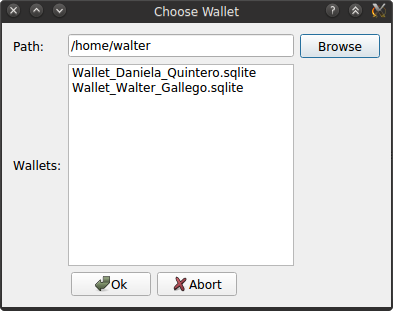
\includegraphics[width=0.48\textwidth]{chapters/figures/development/openWallet.png}}
  {}
  \subfloat[if \texttt{Browse} is clicked a \texttt{QFileDialog} is launched\label{}]{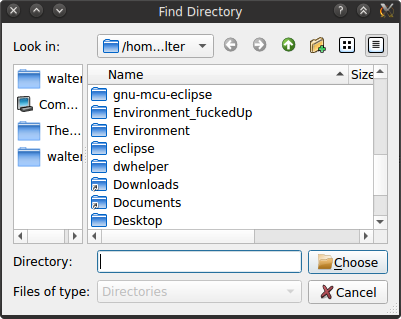
\includegraphics[width=0.48\textwidth]{chapters/figures/development/directories.png}}
  \caption{Open Wallet dialogues}
 \label{fig:openWallet}
\end{figure}

The application proceeds doing the inverse process to the \texttt{Save\_action}, that is, read all the tables from the secure in-disk database and create an in-memory database with this data. To do so, the listings in \ref{lis:openWallet} is used. First, the in-disk data base is opened as read only, and a list named \texttt{tables} with the existent tables in it is generated. Then an in-memory database is created. Finally, for each table in \texttt{tables}, its contents are read, a correspondent table is created in the in-memory database, and the later is populated with the read contents from the in-disk DB.
\begin{lstlisting}[style=customc, float=htb, caption={Simplified Open Wallet action}, label = {lis:openWallet}]
sqlite3_open_v2(fileName.toUtf8(),
                &dbSec, 
                SQLITE_OPEN_READONLY, NULL)); //open in-disk DB

QString tableNames="SELECT name FROM sqlite_master "
                    "WHERE type='table' "
                    "ORDER BY name;";
sqlite3_exec(
  dbSec, tableNames.toUtf8(), 
  callback_createTableList,//builds the 'tables' list 
  this, &zErrMsg);

if (dbMem.isOpen()){ 
  save_table_geometry;
  dbMem.close();//close any prev. opened database
}
dbMem = QSqlDatabase::addDatabase("QSQLITE");
dbMem.setDatabaseName(":memory:");
dbMem.open();
query = QSqlQuery(dbMem);

foreach (const QString table, tables){
  QString sql = "create table '"+table+
                "'(id integer primary key, "
                "Username TEXT, "
                "Domain TEXT, "
                "Password TEXT, "
                "Date TEXT, "
                "Description TEXT );";
  if (table!="NoEmpty"){ //Workaround: ignore empty
    query.prepare(sql);
    query.exec(); //create table in in-mem DB
  }
  QString SqlStatement = 
    QStringLiteral("SELECT * FROM '%1';").arg(table);
  sqlite3_exec(
    dbSec, SqlStatement.toUtf8(), 
    callback_populateTable, //populates in-mem DB
    this, &zErrMsg);
}
\end{lstlisting}


The \texttt{SELECT FROM} statements in \texttt{sqlite3} require the use of a \textsl{callback} function, which is called for every result row, and receive the actual data from the data base as an \texttt{argv[]} argument. In the open process two of these functions are needed, shown in listing \ref{lis:callback}. 
In \texttt{create\_TableList}, the list \texttt{tables} is build by simply reading the only element in the \texttt{argv[]} array, as each row only consists of a table's name. 
In \texttt{populatetable}, the table in the in-memory DB is populated, row by row with each call.  In this case the \texttt{argv[]} array holds the values in a single row coming from the in-disk DB.

Finally the GUI is updated, by enabling some elements and disabling others.

\begin{lstlisting}[style=customc, float=htb, caption={Callback functions for Sqlite3 SELECT}, label = {lis:callback}]
//Build TableList from in-disk DB
callback_createTableList(int argc, char**argv, char**azColName){ 
  tables << argv[0]; //only one arg, the table name
  return 0;
}
//fill 'table' in in-mem DB with data from in-disk DB
callback_populateTable(int argc, char **argv, char **azColName){ 
  if (table=="NoEmpty") // we dont want NoEmpty in the in-mem db
    return 0;
  int i;  

  static const QString insert = 
    QStringLiteral("INSERT INTO '%1' VALUES (%2);");
  
  QStringList values;
  QString aux;
  for(i = 0; i<argc; i++){//argv holds values from a single row 
      aux = argv[i];
      values << "'"+aux+"'"; 
  }
  query.prepare(insert.arg(table).arg(values.join(", ")) );
  query.exec();
  return 0;
}
\end{lstlisting}


\subsubsection*{Close Wallet action}

This action is very simple. As usual, before closing the current wallet a check for unsaved changes is performed, and the user is asked what to do with them using a confirmation dialogue. If the user decides to continue, the in-memory database handler is closed, and the table geometries are saved. Finally the GUI is updated.

\subsubsection*{Delete Wallet action}

Deleting a wallet involves deleting an in-memory database and/or an in-disk database. 

If only the in-memory database exists (user has not save it to disk yet), the wallet is simply closed, as in the previous section.

If there is no opened wallet, and the user wishes to delete an in-disk database, a select file dialogue equal to the one in the \texttt{Open\_Wallet} action is shown, where the user can chose the wallet to delete. Then the wallet is deleted as shown in listing \ref{lis:delete}. First we obtain the encrypted version of the filename, using the SEcube™ API, and then the file in the disk is deleted using standard OS calls. 

\begin{lstlisting}[style=customc, float=htb, caption={Delete an in-disk database}, label = {lis:delete}]
crypto_filename(fileName.toUtf8().data(), 
                enc_filename, &enc_len 
                );
QFile::remove(enc_filename); //OS call
\end{lstlisting}

If both in-disk and in-memory wallets are to be deleted, that is, if there is an opened wallet that has been already saved to disk, there is no need for a select file dialogue, as the filename is known from the \texttt{Save\_Wallet} process. The in-memory database handler is closed and the in-disk encrypted wallet file deleted as explained above. 

In all the above cases, a confirmation dialogue ask the user if they are sure about deleting the wallet.

\subsection{Table actions and display}
Actions and classes regarding tables, they creation and display, are explained in the following sections: 

\subsubsection*{Add Table action}

With an in-memory wallet opened, the user can add a new table to it by simply entering a name. the listing \ref{lis:addTable} shows this process. With the \texttt{QIntputDialog} class, it is possible to ask the user for a name easily. If the name is valid, the sqlite query to add the table is executed. It may be the case the table already exists, in which case the query execution returns an error and the user is notified.

\begin{lstlisting}[style=customc, float=htb, caption={Add a New Table}, label = {lis:addTable}]
bool ok;
QString tableName = QInputDialog::getText
  (this, "New Table",
  "Enter new table name",
  QLineEdit::Normal,"", &ok);

if (!ok || tableName.isEmpty())
  return;

QSqlQuery query(dbMem);
query.prepare("create table '"+tableName+
              "'(id integer primary key, "
              "Username TEXT, "
              "Domain TEXT, "
              "Password TEXT, "
              "Date TEXT, "
              "Description TEXT )");

if (!query.exec()){
  return; // maybe a table with that name already exists, or is a reserved SQLite command
\end{lstlisting}

If the table is the first one to be added in the wallet, a \texttt{table view} and \texttt{filters} are created and added to the GUI, in order to display the table. Otherwise, the \texttt{table view} is just updated. These elements are explained in details in the upcoming sections.

\subsubsection*{Delete Table action}

To delete a table it is enough to use the SQLite \texttt{DROP TABLE} command as seen in listings \ref{lis:deleteT}. With the \texttt{QMessageBox} the user is asked to confirm before deleting.

After deleting, the \texttt{table view} needs to be updated, to show the next table in the wallet. If there are no more tables, the view is simply hidden, and other GUI elements like \texttt{Add Entry} disabled.

\begin{lstlisting}[style=customc, float=htb, caption={Delete Table}, label = {lis:deleteT}]
reply = QMessageBox::question
          (this,
          "Delete",
          "Are you sure you want to delete Table "+tableName,
          QMessageBox::Yes|QMessageBox::No);
if (reply == QMessageBox::No)
  return;

QSqlQuery query(dbMem);
query.prepare("DROP TABLE '" + tableName+"'");
\end{lstlisting}

\subsubsection*{Rename Table action}
To Rename a table the SQLite command \texttt{ALTER TABLE RENAME TO} is used as seen in listing \ref{lis:renameT}. After this, the \texttt{QComboBox} used to select the current table being displayed is updated to reflect the name change.
\begin{lstlisting}[style=customc, float=htb, caption={Rename Table}, label = {lis:renameT}]
QSqlQuery query(dbMem);
query.prepare("ALTER TABLE '" + currentName + "' RENAME TO '"+newName+"'");
query.exec();
\end{lstlisting}

\subsubsection*{Select Table}

To allow the user to select one table to display out of the existent ones in the current Wallet, a \texttt{QComboBox} is added to the Entries Tool Bar. Each time a Wallet is opened/closed, or a table is added/renamed/deleted, the items in the QComboBox are updated accordingly. When the selected item in the QComboBox changes, the tableView update procedure explained in the following section is triggered.

\subsubsection*{Table display}
To display the entries in each of the Wallet tables, a \textbf{Model/View} architecture was followed. From the official Qt documentation \cite{modelview}:
 
``Model-View-Controller (MVC) is a design pattern originating from Smalltalk that is often used when building user interfaces. In Design Patterns, Gamma et al. write:

MVC consists of three kinds of objects. The Model is the application object, the View is its screen presentation, and the Controller defines the way the user interface reacts to user input. Before MVC, user interface designs tended to lump these objects together. MVC decouples them to increase flexibility and reuse.

If the view and the controller objects are combined, the result is the \textbf{model/view} architecture. This still separates the way that data is stored from the way that it is presented to the user, but provides a simpler framework based on the same principles.''

``The model communicates with a source of data, providing an interface for the other components in the architecture. The nature of the communication depends on the type of data source, and the way the model is implemented.

The view obtains model indexes from the model; these are references to items of data. By supplying model indexes to the model, the view can retrieve items of data from the data source.

In standard views, a delegate renders the items of data. When an item is edited, the delegate communicates with the model directly using model indexes.''

Figure \ref{fig:modelview} (taken from the Qt documentation), shows the way these three elements interact between them and with the data. 

\begin{figure}[htb]
  \centering
  \captionsetup{justification=centering}
  \centerline{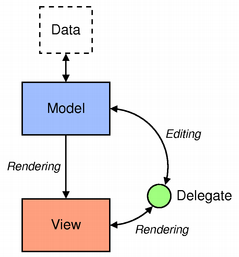
\includegraphics[width=0.5\columnwidth]{chapters/figures/development/modelview.png}}
  \caption{The Qt Model View Architecture}
  \label{fig:modelview}
\end{figure}

\begin{lstlisting}[style=customc, float=htb, caption={Model/View architecture implementation}, label = {lis:modelview}]
// Create and configure model to access data in table
model = new QSqlTableModel;
model->setTable(tableName);
model->select();//update the model selection
model->setEditStrategy(QSqlTableModel::OnManualSubmit);
  //Changes will be updated manually by calling submitAll()

//Create ProxyModel for filtering
proxyModel = new MySortFilterProxyModel(this);
proxyModel->setSourceModel(model); //connect proxyModel to Model

//Create and connect delegate to hide passwords
passDelegate=new PasswordItemDelegate(this);
ui->tableView->setItemDelegateForColumn(PASS_COL, passDelegate);

//Connect to table view, resulting in: 
//Sql <--> Model <--> ProxyModel <--> Delegate <--> TableView
ui->tableView->setModel(proxyModel);

//Configure table
ui->tableView->//Hide SQLite ID column, not useful to user
  setColumnHidden(IDENT_COL, true);
ui->tableView->//Hide row header, not useful
  verticalHeader()->hide();
ui->tableView->//To make the table view not editable
  setEditTriggers(QAbstractItemView::NoEditTriggers);
ui->tableView->//To allow only one row  selection.
  setSelectionBehavior(QAbstractItemView::SelectItems);
ui->tableView->//So we can edit one entry per time
  setSelectionMode(QAbstractItemView::SingleSelection);

ui->tableView->show();// show table
\end{lstlisting}

In the SEcubeWallet application these elements correspond to:

\begin{itemize}
\setlength\itemsep{-3pt}

\item \textbf{Data:} The data coming from the database. As we are displaying only one table at a time, the data actually corresponds to a single table.
\item \textbf{Model}: \texttt{QSqlTableModel}, a Qt class which provides an editable data model for a single database table.
\item \textbf{Proxy Model}: \texttt{MySortFilterProxyModel}, a class written by the author inheriting from the Qt \texttt{QSortFilterProxyModel} class. It implements custom filtering for each of the columns, in particular for the date.
\item \textbf{View}: \texttt{MyQTableView}, a class written by the author inheriting from the Qt \texttt{QTableView} class. \texttt{MyQTableView} reimplements the \texttt{resizeEvent} to make sure the user has the best GUI experience. This new class allows for manual resizing of each column as well as automatic resizing when the widow size changes. Also, there is a button that allows the user to fit the table in the available space by giving all the columns the same width.
\item \textbf{Delegate}: \texttt{PasswordItemDelegate}, a class written by the author inheriting from the Qt \texttt{QStyledItemDelegate} class. It is used to implement the show/hide password functionality.
\end{itemize}

There is one element not mentioned in the model/View architecture: the \textbf{Proxy Model}. It will be explained in details in the filters section. The \textbf{delegate} will be explained in the Show Password section.

In listing \ref{lis:modelview} the model view architecture is implemented. Model, Proxy Model and Delegate are interconnected among them, with the database table and with the GUI's table view. Additionally some display tweaks are made, for instance the ID column, vertical header and passwords are hidden.



When it is necessary to change the table to be displayed, either because the user changes walllet or table, or deletes one, the listing \ref{lis:updatemv} is used. Only the \textbf{model} needs to be updated, because it is the one connected to the data. The table view geometry needs to be saved and restored, because with the data change, the columns are automatically resized by Qt to fit the new data, which is visually annoying for the user.

\begin{lstlisting}[style=customc, float=htb, caption={update the model/view}, label = {lis:updatemv}]
save_table_geometry;//each column width
model->setTable(tableName);
model->select();
    
restore_table_geometry;
ui->tableView->setColumnHidden(IDENT_COL, true);//required
\end{lstlisting}

\subsubsection*{Show Passwords action}

To show the passwords it is enough to \textsc{not} use a delegate for the correspondent column. Conversely, to hide them again, the delegate is used, as seen in listing \ref{lis:pass}. The delegate \texttt{displayText} method definition is also shown. Its job is to return the bullet character eight times instead of the actual item value.

\begin{lstlisting}[style=customc, float=htb, caption={Show/Hide Passwords}, label = {lis:pass}]
// *** in pasworditemdelegate.cpp ***
PasswordItemDelegate::PasswordItemDelegte(QObject* parent): QStyledItemDelegate(parent){}
//inherits from QStyledItemDelegate

QString PasswordItemDelegate::displayText
  (const QVariant &value, const QLocale &locale) const {
    return (QString("%1").arg(QChar(0x2022)).repeated(8));
} // just returns the bullet character 8 times

// *** in mainwindow.cpp ***
void MainWindow::on_action_Show_Passwords_toggled(bool show){

	passDelegate=new PasswordItemDelegate(this);
	if (!show)//do not show passwords: use passDelegate
	  ui->tableView->setItemDelegatForColumn(
	    PASS_COL, passDelegate);
	 
	else{ //show passwords: do not use delegate
	  QMessageBox::StandardButton reply;
	  reply = QMessageBox::question(
	            this,
	            "Passwords",
	            "Are you sure you want to show your passwords",
	            QMessageBox::Yes|QMessageBox::No);
	  if (reply == QMessageBox::No)
	    return;//if error or cancel, do nothing
	
	  ui->tableView->setItemDelegateForColumn(PASS_COL, 0);
	}
}
\end{lstlisting}

\subsubsection*{Filters}
The filters implementation comprise two classes. The first one is related to the GUI, and its job is to align each of the filters with its corresponding table column. The second class is related to the data filtering per se.

The \textbf{filters alignment} is based on the \texttt{ColumnAlignedLayout} class by sashoalm \cite{aligned}. This class is a Layout that inherits from the \texttt{QHBoxLayout} Qt class. It reimplements the \texttt{setGeometry} method to reposition each of the elements in the layout to follow the correspondent column in the tableView that is being tracked. This implementation allows to add any type of widget to the layout, as long as the number of widgets equals the number of tracked columns. The class definition is shown in listing \ref{lis:aligned}.

\begin{lstlisting}[style=customc, float=htb, caption={Aligned Filters definition}, label = {lis:aligned}]
// *** filtersaligned.cpp ***
FiltersAligned::FiltersAligned(QWidget *parent) //constructor
: QHBoxLayout(parent){//inherits from horizontal Box Layout
  add_filters_to_layout; //add filters (most of them QLineEdits)
}
void FiltersAligned::setTableColumnsToTrack(QHeaderView *view) {
    headerView = view; //set tracked tableView
}
void FiltersAligned::setGeometry(const QRect &r){
  QHBoxLayout::setGeometry(r);

  int widgetX = parentWidget()->mapToGlobal(QPoint(0, 0)).x();
  int headerX = headerView->mapToGlobal(QPoint(0, 0)).x();
  int delta = headerX - widgetX;

  // repositioning
  for (int ii = 0; ii < headerView->count(); ++ii) {
    int pos = headerView->sectionViewportPosition(ii);
    int size = headerView->sectionSize(ii);
    auto item = itemAt(ii);
    auto r = item->geometry();
    r.setLeft(pos + delta);
    r.setWidth(size);
    item->setGeometry(r);
  }
}
\end{lstlisting}

To connect the aligned layout to the table view, the listing \ref{lis:alignedcon} is used. In it, an aligned filter object is created and is set as the Layout of a widget positioned over the tableView in the GUI. Then the aligned filter is set to track the tableView's \texttt{horizontalHeader}. Finally any geometry change in the \texttt{horizontalHeader}, or in the \texttt{horizontalScrollBar} calls the \textsc{slot} \texttt{invalidateAlignedLayout}, which in turns calls the \texttt{invalidate} method. This method resets the Layout's cached information, which forces a call to \texttt{setGeometry}. This ensures any resizing of the table's columns is reflected in the filters position.


\begin{lstlisting}[style=customc, float=htb, caption={Table View and aligned filters connection}, label = {lis:alignedcon}]
// *** in mainwindow.cpp when the tableView is created:
  filters = new FiltersAligned();
  ui->filtersWidget->setLayout(filters);
  filters->setTableColumnsToTrack(
    ui->tableView->horizontalHeader());
  filters->setParent(ui->filtersWidget);
  
  connect(ui->tableView->horizontalHeader(),
          SIGNAL(sectionResized(int,int,int)), 
          SLOT(invalidateAlignedLayout()));
  connect(ui->tableView->horizontalScrollBar(), 
          SIGNAL(valueChanged(int)),
          SLOT(invalidateAlignedLayout()));

//the SLOT
void MainWindow::invalidateAlignedLayout(){
    filters->invalidate(); 
}//clears the cache, which forces a call to setGeometry
\end{lstlisting}


The \textbf{data filtering} is done using a custom \texttt{SortFilterProxyModel}. For all the columns except the date, a simple case insensitive match is enough. For the date, using a button in the GUI, the user can choose among two options:

\begin{itemize}
\setlength\itemsep{-3pt}

\item \textbf{Exact Match filter: }In this configuration, the user enters the exact date they are looking for, using a \texttt{QDateEdit} input element.
\item \textbf{Older Than filter: }Because this is a password wallet, looking for an exact date may not be very useful. Instead, knowing which passwords are older than a given amount of time, and have therefore expired is more helpful. For instance the user could be interested in updating their passwords each six months, so with this filter they can show only those passwords that need to be changed. In figure \ref{fig:filterdate} an Older Than six months filter is shown (as of July the 13th 2018).
\end{itemize}

\begin{figure}[ht]
  \centering
  \subfloat[No filter\label{}]{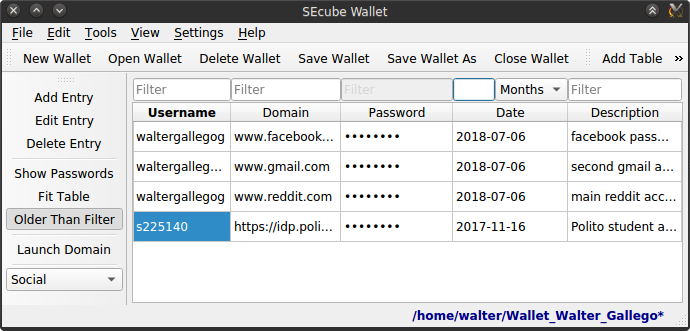
\includegraphics[width=0.48\textwidth]{chapters/figures/development/filterdatea.png}}
  {}
  \subfloat[Older Than 6 Months\label{}]{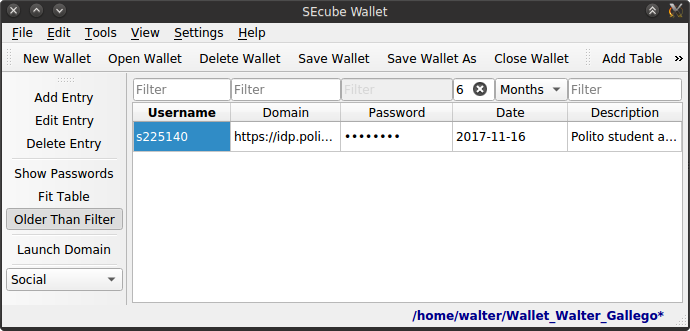
\includegraphics[width=0.48\textwidth]{chapters/figures/development/filterdateb.png}}
  \caption{Date Older Than filter }
 \label{fig:filterdate}
\end{figure}

The filters implementation is very simple. It involves the reimplementation of the \texttt{filterAcceptsRow} method in the ProxyModel as in listings \ref{lis:filterReg}. This method  is called each time the user changes one of the filters contents. The filters work concurrently, so the user can search in multiple columns at the same time. All of them except the date one accept \texttt{RegExp}, so a search like \texttt{google|gmail} is possible. The password filter is only enabled when the passwords are visible.


\begin{lstlisting}[style=customc, float=htb, caption={Filters implementation}, label = {lis:filterReg}]
bool MySortFilterProxyModel::filterAcceptsRow
(int sourceRow, const QModelIndex &sourceParent) const
{
  QModelIndex userIndex = 
    sourceModel()->index(sourceRow, USER_COL, sourceParent);
  QModelIndex domainIndex = 
    sourceModel()->index(sourceRow, DOM_COL, sourceParent);
  QModelIndex passIndex = 
    sourceModel()->index(sourceRow, PASS_COL, sourceParent);
  QModelIndex descIndex = 
    sourceModel()->index(sourceRow, DESC_COL, sourceParent);

  QModelIndex dateIndex = 
    sourceModel()->index(sourceRow, DATE_COL, sourceParent);
  QDate thisDate = QDate::fromString(
    sourceModel()->data(dateIndex).toString(),format);

  return (//only return rows where the conditions are met    
    sourceModel()->
      data(userIndex).toString().contains(userRegExp)         && 
    sourceModel()->
      data(domainIndex).toString().contains(domainRegExp)     && 
    sourceModel()->
      data(passIndex).toString().contains(passRegExp)         &&
    sourceModel()->
      data(descIndex).toString().contains(descRegExp)         &&
    (thisDate<=filterDate_older||!filterDate_older.isValid()) &&
    (thisDate==filterDate_exact||!filterDate_exact.isValid()) &&
  );
}
\end{lstlisting}

\subsection{Entries actions}

In this section, the implementation of the actions add/edit/delete entry are explained.

\subsubsection*{Add Entry action}

The \texttt{AddEntry} class allows users to input a new entry to one of the tables, using the subwindow in figure \ref{fig:addentry}

\begin{figure}[ht]
  \centering
  \subfloat[Passwords are shown and do not match\label{fig:addentrya}]{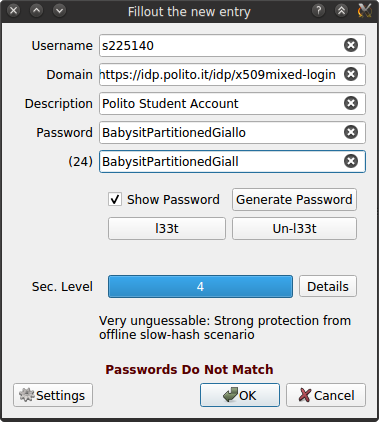
\includegraphics[width=0.32\textwidth]{chapters/figures/development/addEntrya.png}}
  {}
  \subfloat[Passwords are shown and do match\label{fig:addentryb}]{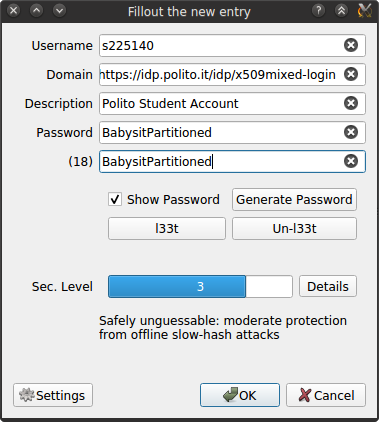
\includegraphics[width=0.32\textwidth]{chapters/figures/development/addEntryb.png}}
  {}
  \subfloat[Passwords are shown. zxcvbn library has not been compiled\label{fig:addentryc}]{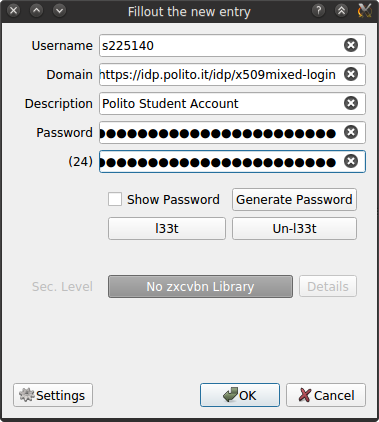
\includegraphics[width=0.32\textwidth]{chapters/figures/development/addEntryc.png}}
  \caption{Add Entry subwindow}
 \label{fig:addentry}
\end{figure}

This subwindow is composed of:

\begin{itemize}
\setlength\itemsep{-3pt}

\item \textbf{Text input elements: }To enter the Username, Domain, Description and Password, five \texttt{QLineEdit} are used. The password needs to be entered twice to make sure is the desired one, and if it is not the same in both text fields, an error message is displayed. The date is not entered by the user, but generated automatically based on the system clock.
\item \textbf{Show password checkBox: }By changing the echo mode in the password \texttt{QLineEdit}, it can be hidden or shown. It is hidden by default
\item \textbf{Password Generator Button: }This triggers one of two available generators: PwGen or PassPhraseGen. These are explained in detail in sections \ref{sec:pwgen} and \ref{sec:ppgen}
\item \textbf{l33t buttons: }To increase the password strength the user can translate it to l33t. If they are not happy with the result, a button to reverse the action is also present. The l33t implementation is explained in section \ref{sec:l33t}
\item \textbf{Password Strength elements: } A Progress Bar used to display the password strength calculated with the zxcvbn library, a label to show some information about the strength, and a button to open a subwindow showing the details of these calculations. If the zxcvbn library has not been compiled by the user in the settings window, these elements are disabled. The zxcvbn library is explained in details in section  \ref{sec:zxcvbnim}
\item \textbf{Bottom buttons: }The \texttt{ok} button is only functional when all the text fields (except for \texttt{description}, which is optional) are filled, and the two passwords coincide. The \texttt{settings} button opens the settings subwindow so the user can customize the password generators or the strength estimator without having to close the \texttt{AddEntry} subwindow.

\end{itemize}

When the user clicks the \texttt{ok} button, the new entry needs to be added to the database. Instead of using SQLite commands, it is easier to rely in the high-abstraction level methods offered by the \texttt{model}, as seen in listing \ref{lis:addtomodel}.


\begin{lstlisting}[style=customc, float=htb, caption={Add entry to database using model}, label = {lis:addtomodel}]
AddEntry *add = new AddEntry(this);
add->exec(); //exec AddEntry subwindow
if(add->result()==QDialog::Rejected)
  return; // Error or cancel, do nothing

QSqlRecord rec = model->record(); // Temp entry
rec.setGenerated("id", false); // is managed by SQLite

//Get the values entered by user in AddEntry subwindow
rec.setValue("Username"   , add->getUser());
rec.setValue("Password"   , add->getPassword());
rec.setValue("Domain"     , add->getDomain());
rec.setValue("Description", add->getDescription());

rec.setValue("Date",        QDate::currentDate());//sys clock

int newRecNo = model->rowCount(); //insert at the end of table
if (!model->insertRecord(newRecNo, rec))
  return;
model->submitAll();// if insert ok, submit changes.
\end{lstlisting}

\subsubsection*{Edit Entry action}

The user can edit any of the entries by selecting one of the cells in the \texttt{tableView} and clicking the \texttt{Edit Entry} button, or by double-clicking any of the cells. In either case, the data from the selected row is retrieved and passed to new \texttt{AddEntry} object using its constructor. In this way, the user is presented with an \texttt{AddEntry} subwindow where the input fields are already filled with the current data. The user can then modify and save them by clicking \textsc{ok}. In this process the \texttt{ProxyModel} is used instead of the \texttt{model}, because the former allows to identify the items selected in the \texttt{tableView}.

\subsubsection*{Delete Entry action}

Deleting an entry is very simple. The row index of the selected cell is used in the \texttt{ProxyModel} method \texttt{removeRow(row)}, and the change is submitted with \texttt{submitAll}. Before deleting, the user is asked to confirm the action.

\subsection{Other functionalities}
In this section, a set of miscellaneous functionalities are explained.

\subsubsection*{Launch Domain action}

Using the Qt function \texttt{QDesktopServices::openUrl(QUrl(domain))}, it is straight forward to open the domain of the entry selected by the user. It will be opened in the default web browser configured in the OS. The only detail to play attention is the format. If the domain entered by the user does not start with \texttt{http://} or \texttt{https://}, then \texttt{http://} is prepended. Also, if the entered domain does not contain any dots apart from the one in \texttt{www.}, then the most common top-level domain, \texttt{.com} is added. This will not work in all the cases, but should help fixing some of the domains when the user forgets to type the TLD.


\subsubsection*{Status Bar}
The status bar, at the bottom of the main window, is used to display three types of information:

\begin{itemize}
\setlength\itemsep{-3pt}

\item \textbf{Wallet Name: }The wallet name (with full path) is permanently displayed at the right side of the status bar in color blue. In case the wallet does not have a name because the user has not saved yet, \texttt{unnamed} is displayed. When the wallet has unsaved changes, an asterisk is added to the end resulting in: \texttt{/absolute\_path/wallet\_name*} 

\item \textbf{Success: }After any save/open/delete operation, a black message is shown for two seconds in the left side of the status bar, informing the user the process concluded without issues.

\item \textbf{Error/Warning: }In the eventuality of an error or warning during the execution of a command, for instance, if it is not possible to load the SQLite driver, a red message in the left side of the status bar informs the user about the issue.
\end{itemize}


\subsubsection*{Preferences Subwindow}

This subwindow is accessible from the \texttt{Menu Bar} and from the \texttt{AddEntry} subwindow. It allows to customize the password generators and the strength estimator. Their available configurations are covered in their respective sections. 

\subsubsection*{Environment subwindow}

From the environment subwindow the user can select which of the keys and algorithms present in the SEcube™ chip to use for the encryption/decryption process. 

Keys are used to divide wallets into categories (work, banking, social) and allow their sharing.  A given user can have for instance one key that is shared among co-workers, so all of them can access work-related passwords using their respective SEcube™ devices. Similarly, other key can be shared with their family to access banking accounts passwords, and finally have a personal key that is not shared with anyone and is used to encrypt social media passwords. 

The current SEcube™ firmware version only includes one algorithm for the data encryption/decryption process, but in the future it may provide more than one. Different algorithms offer different security characteristics that some advance user may find useful. For example one user could be concerned about some specific type of attack that requires an special algorithm, or regard one algorithm superior over the others. 

Figure \ref{fig:envi} depicts the environment subwindow.

\begin{figure}[htb]
  \centering
  \captionsetup{justification=centering}
  \centerline{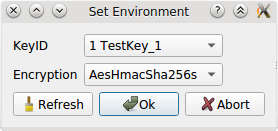
\includegraphics[width=0.5\columnwidth]{chapters/figures/development/envi.png}}
  \caption{Environment subwindow}
  \label{fig:envi}
\end{figure}


\subsubsection*{Help Subwindow}

This subwindow teaches the user a few tips about how to use the application features, some of which may not be obvious, like the strength estimator or the date filter. It also  gives some information about the application, like the author, year, and code sources.



\subsubsection*{l33t} \label{sec:l33t}

This is a very simple converter that uses the capabilities of the \texttt{QString} class to replace each occurrence of the letters \texttt{o i z E A s b T B P} with the numbers \texttt{0 1 2 3 4 5 6 7 8 9} respectively, and the letter \texttt{l} with the character \texttt{|}. To un-l33t, the reverse process is made. It is worth noticing that password crackers (and strength estimators like zxcvbn) usually try an l33t dictionary too, so this option may increase the password strength, but not by too much. In table \ref{tab:l33t} a few passwords and their l33t version are compared. The strength measured with zxcvbn is reported.

\begin{table}[ht]
\renewcommand{\arraystretch}{1.3}
\centering
\caption{A few l33t examples}
\begin{tabular}{lr}
\toprule
\textbf{Password} & \textbf{Log Entropy (Level)} \\ \midrule

LeytonVariational & 9.44 (Level 3) \\
Leyt0nVar1at10na| & 10.22 (Level 4) \\
\midrule
PenicuikCiting & 9.09 (Level 3) \\
9en1cu1kC1t1ng & 13.87 (Level 4) \\
\midrule
LauraDrogheda & 6.44 (Level 3) \\
LauraDr0gheda & 6.74 (Level 4) \\

\bottomrule
\end{tabular}
\label{tab:l33t}
\end{table}

\subsection{PwGen: Pronounceable Passwords Generator} \label{sec:pwgen}
As seen from previous sections, the PwGen program is open source and available in the official Linux repositories. A very simple way of including its functionalities into the SEcubeWallet application would be to use a \texttt{Qprocess} to call PwGen as an external program. Although is tempting to use this solution because of its simplicity, there are three drawbacks with this approach:

\begin{enumerate}
\setlength\itemsep{0pt}
\item It would require for the user to install the PwGen program, as it is usually not included in common Linux distributions.
\item It would not be very portable, because even if there is a PwGen version for windows, the available version or input parameters could differ in different platforms.
\item Security could be compromised. As PwGen needs to communicate the generated password back to the SEcubeWallet application, an attacker could steal the password in this process.
\end{enumerate}

For these reasons, it was decided to embed the PwGen sources directly into the application, this ensure the password never leaves the application memory space. 
To include the sources into the application, some slight modifications (mostly simplifications) to the PWGen \texttt{main()} function were necessary. This is because the original sources are intended for the use of PwGen as a independent console program called by users, so the \texttt{main()} contains code dedicated to parse the input arguments in the standard \texttt{argc argv[]} fashion. Only the \texttt{pwgen.c} and \texttt{pwgen.h} --- files where the \texttt{main()} is implemented --- were modified.

\subsubsection*{Options GUI}
As all the options for PwGen besides the password length are yes or no questions, the checkable list shown in figure \ref{fig:pwgenSett} is perfect for this purpose.

\begin{figure}[htb]
  \centering
  \captionsetup{justification=centering}
  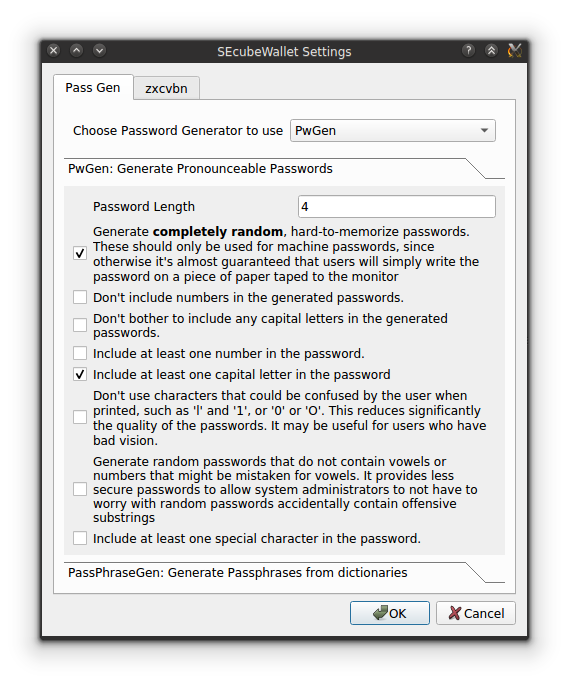
\includegraphics[width=0.8\columnwidth]{chapters/figures/development/pwgenSett}
  \caption{PwGen settings in the preference window}
  \label{fig:pwgenSett}
\end{figure}

When the \texttt{OK} button is clicked, all the values are saved using the \texttt{QSettings} class, so they are available even after restarting the application.

\subsubsection*{Usage}

When the \texttt{Generate Password} button in the \texttt{AddEntry} class is clicked, the settings values stored in with the \texttt{QSettings} class are read and from them a \texttt{char[]} with the PwGen options syntax is built. Before calling the Generator, it is necessary to allocate a memory space equal to the desired password length (in \texttt{char}) and pass this buffer as a pointer (\texttt{char*}) to PwGen. PwGen will write the generated password in this space. This steps can be seen in the listing \ref{lis:pwgen}


\begin{lstlisting}[style=customc, float=htb, caption={PwGen call inside AddEntry}, label = {lis:pwgen}]
//read user settings (if existent)
if (settings.value("passGens/pwgen/1cap").toBool())
    options.append("c");
if (settings.value("passGens/pwgen/1num").toBool())
    options.append("n");
if (settings.value("passGens/pwgen/1spec").toBool())
    options.append("y");
if (settings.value("passGens/pwgen/noAmb").toBool())
    options.append("B");
if (settings.value("passGens/pwgen/noCap").toBool())
    options.append("A");
if (settings.value("passGens/pwgen/noNum").toBool())
    options.append("0");
if (settings.value("passGens/pwgen/noVow").toBool())
    options.append("v");
if (settings.value("passGens/pwgen/random").toBool())
    options.append("s");

//check if user entered an integer, if not, default is 16
if(settings.value("passGens/pwgen/len").toInt())
    length = settings.value("passGens/pwgen/len").toInt();

//allocate space for password
buf = (char*)malloc(length+1);
if(!buf){
  return;//error, could not allocate
}
//actual call to password generator
main_pwgen(
  options.length(),               //int, number of options 
  options.toLatin1().constData(), //char *, options 
  length,                         //password length 
  buf                             //char *, to return the password           
);
genPass = QString::fromLatin1(buf,length);
free(buf);
\end{lstlisting}

\subsubsection*{Results}

A few examples of the resulting Passwords are show in table \ref{tab:pwgenExm}, with their respective zxcvbn Log entropy score and Level. As expected, the passwords with highest entropy are those obtained using the \texttt{-s} (Random) and \texttt{-sy} (Random and especial characters) options. Even with only 6 characters it is possible to get a Level 4 password like \texttt{TBw4)9}. The drawback is, they are hard to remember and type. 

On the contrary, a password obtained with the \texttt{-BA0} (No ambiguous, do not capitalize, no numbers, pronounceable) options, like \texttt{nofosootei}, only reaches a Level2, but it is very easy to remember and type.

\begin{table}[ht]
\renewcommand{\arraystretch}{1.3}
\centering
\caption{A few PwGen generated passwords}
\begin{tabular*}{\columnwidth}{
@{\extracolsep{\fill}}
m{4cm}ccr
@{}}
\toprule
\hd{Password} & \hd{Length} & \hd{Options} & \hd{Log Entropy \\ \& Level}  \\ \midrule

iesohGhai3   & 10 & -   &  9.75 (Level 3)\\
ees0cooLo2   & 10 & -   & 10.47 (Level 4)\\
dX042wKqlW   & 10 & s   & 17.86 (Level 4)\\
@!,Q*l5\}+H  & 10 & ys  & 18.15 (Level 4)\\
TBw4)9       &  6 & ys  & 11.62 (Level 4)\\
B7t34Lck     &  8 & v   & 11.87 (Level 4)\\
nofosootei   & 10 & BA0 &  6.50 (Level 2)\\
\bottomrule  
\end{tabular*}
\label{tab:pwgenExm}
\end{table}

\subsection{zxcvbn Password strength estimator} \label{sec:zxcvbnim}

The original zxcvbn project, developed in CoffeeScript became so popular it was ported to a large variety of languages. In this work the C/C++ version available at \cite{zxgit} was used. The files used in this project are:

\begin{itemize}
\setlength\itemsep{-3pt}

\item \textbf{zxcvbn.c} Main source file
\item \textbf{zxcvbn.h} Main header file
\item \textbf{dict-generate.cpp} Used for generating the dictionary sources
\item \textbf{Makefile} To compile the dictionary generator and main program.
\item \textbf{words-*.txt} A few examples of dictionary files in plain text format.
\end{itemize}

Besides source files, zxcvbn also needs to compile the dictionary files, but first lets define what is a dictionary, why are they important and why they need to be compiled (For general dictionaries only. User dictionaries are small and can be added at runtime).

\subsubsection*{General dictionaries}

Dictionaries are a crucial part of the algorithm, because they are used estimate the security level of a password according to how common the used words (if any) are. A password containing words present in any of the dictionaries will be easier to crack as hackers will probably try out those specific words or a combination of them.

General dictionaries contain a large number of words that are useful for all users. Examples of these type of dictionaries (included in this work) are:
\begin{itemize}
\setlength\itemsep{-3pt}

\item 100000 English words from wikipedia.
\item 88800 Last names from the US census database
\item 39000 English words from tv and film from the wikiproject \cite{wiktionary}
\item 47000 Most common passwords from Burnett \cite{burnett}
\item 15480 Italian words from the \textsc{badip} project \cite{badip} 
%TODO
\todo{More dicts, see bookmarks}
\item 4276 Female names from the US census database 
\item 1220 Male names from the US census database
\end{itemize} 

As the dictionary files in plain text are pretty large, the algorithm does not read from them directly. Instead, a \texttt{DicNodes} array is generated, using the tool \texttt{dict-generate}, and this array is compiled into the source code.
To add their own dictionaries, the users need to make sure they are saved as plain-text, (.txt UTF-8), and stored into the zxcvbn directory. The files must have one word per line, with the first word being the most common one. So for instance, in the English dictionary the first word is \texttt{the} and the last one is \texttt{surma}. This is important as it is used to calculate the entropy of the passwords. A password containing the word \texttt{surma} is far more secure that one containing the word \texttt{the}.

\subsubsection*{Static Library vs Shared Library}

Because the dictionaries are transformed into a source file and then compiled together with the main program, it is not possible to add, remove or modify dictionary files after the sources are compiled. Therefore the zxcvbn library can not be embedded into the SEcubeWallet application as a static library (or using the C sources directly), but rather, a \textbf{shared library} approach was followed, which allows the dynamic unload/update/load of the library. This has some performance penalties over static libraries, but it is the only way to give the users the possibility of customize the dictionaries as they please.

\subsubsection*{Compilation process}

The steps performed by the \texttt{makefile} in order to compile the dictionaries and sources are:

\begin{enumerate}
\setlength\itemsep{-3pt}

\item Compile the source file \texttt{dict-generate.cpp} to obtain the dict generator executable\texttt{dictgen}.
\item Execute \texttt{dictgen} with the names of dictionaries to process as input argument. As a result the file \texttt{dict-src.h} is created.
\item Compile the files \texttt{zxcvbn.c} and \texttt{zxcvbn.h} together with the just generated \texttt{dict-src.h}, using the gcc flag \texttt{-fPIC} so the resulting object file \texttt{zxcvbn-inline-pic.o} is suitable for library inclusion.
\item Generate the shared library \texttt{libzxcvbn.so} from the object file. This is the library used by the SEcubeWallet sources.
\end{enumerate}

The compilation process can be started by the user from the preference window, where they can also select the dictionaries to use, or clean the generated files. The compiling is made with OS calls, through the use of \texttt{QProcess}. To avoid the application from crashing or getting stuck, the \texttt{Qprocess} has a timeout. As the compile process may take a while depending on the dictionaries size, this timeout can be configured by the user. In figure \ref{fig:zxcvbnGen} the GUI for these actions is shown.

\begin{figure}[ht]
  \centering
  \subfloat[Tab dedicated to zxcvbn preferences]{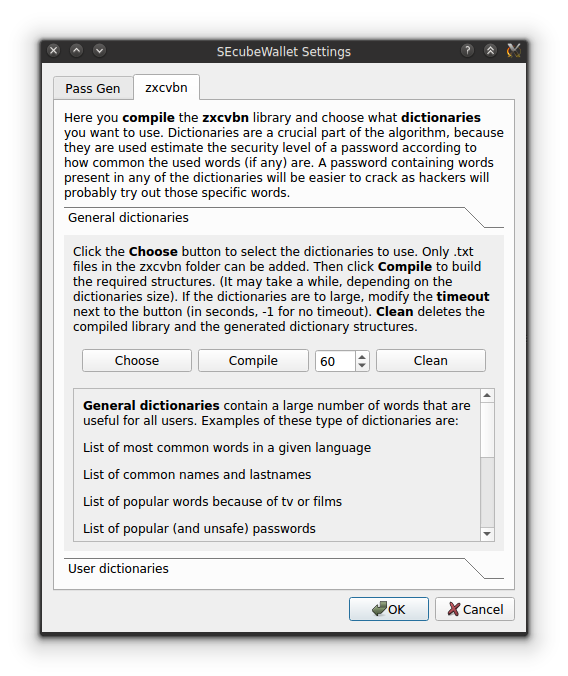
\includegraphics[width=0.5\textwidth]{chapters/figures/development/zxcvbnGen.png}}
  \subfloat[Checkable dialogue to enable dictionaries, appears after clicking the Choose button]{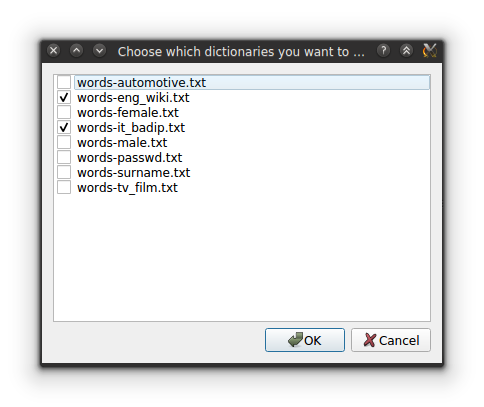
\includegraphics[width=0.4\textwidth]{chapters/figures/development/dictListSett.png}}
  \caption{zxcvbn general dictionaries configuration}
 \label{fig:zxcvbnGen}
\end{figure}

\subsubsection*{Dynamic Library loading}

To manage the zxcvbn shared library at runtime it is possible to use the qt class \texttt{Qlibrary}, which provides access to the functionality in the library in a platform independent way. To use it, is necessary to pass as argument to the constructor the path to the library. Then load it and resolve the desired functions. If no errors are found, the functions can be used as usual. Finally unload the library when it is not needed any more. See Listing \ref{lis:qlibrary}.


\begin{lstlisting}[style=customc, float=htb, caption={Qlibrary basic usage}, label = {lis:qlibrary}]

/***** In header file *****/
//Main zxcvbn function type
typedef double (*ZxcvbnMatch_type)(const char *Passwd, 
                                   const char *UserDict[], 
                                   ZxcMatch_t **Info );
//Function used to free the Info structure
typedef void (*ZxcvbnFreeInfo_type)(ZxcMatch_t *Info);

QLibrary * zxcvbnLib = 0;
ZxcvbnMatch_type ZxcvbnMatch = 0;
ZxcvbnFreeInfo_type ZxcvbnFreeInfo = 0;

/***** In cpp file *****/     
zxcvbnLib = new QLibrary(zxcvbn_lib_path);
    
if(zxcvbnLib->load()){
  ZxcvbnMatch = (ZxcvbnMatch_type) zxcvbnLib->resolve("ZxcvbnMatch");
  ZxcvbnFreeInfo =(ZxcvbnFreeInfo_type) zxcvbnLib->resolve("ZxcvbnFreeInfo");
}

if (!ZxcvbnMatch || !ZxcvbnFreeInfo ){
  //error: Any of the two functions was not resolved correctly
else{
  //we can use the functions normally
  
//When not needed any more
zxcvbnLib->unload();
ZxcvbnMatch = 0;
ZxcvbnFreeInfo = 0;
free(zxcvbnLib);  
  
\end{lstlisting}


\subsubsection*{User Dictionaries}

The user dictionary contain words that are relevant only to a specific user. For example, if the application is used to increase the strength level of passwords used by employees in a company, adding the company's name to the dictionary is a good idea. Furthermore, if the company works in the automotive business, related words as motor, aerodynamic, wheels etc. should be added. By adding those words to the user dictionary, the strength level of passwords using them will decrease, and so the user will be encouraged to never use words that are too easy to guess. The key to a good password is in its randomness. When a hacker is trying to crack one, they will for sure try words relevant to the target.

From the GUI the user can add words manually, or can load them from a text file, but as the words are saved as a simple array, the text file size should not be too large. For large files, it is better to add them as General dictionaries.

\subsubsection*{Estimator Usage}

After the library is loaded and the functions resolved, to use the estimator one simply needs to call the main function \texttt{ZxcvbnMatch} whose declaration we see in Listing \ref{lis:zxcvbn} 

\begin{lstlisting}[style=customc, float=htb, caption={ZxcvbnMatch function declaration}, label = {lis:zxcvbn}]
double ZxcvbnMatch(       //Returns: entropy value in bits.
 
  const char *Passwd,     //The password to be tested. Null terminated string. 
  
  const char *UserDict[], //User supplied dictionary words to be considered particulary bad. Passed as a pointer to array of string pointers, with null last entry (like the argv parameter to main()). May be null or point to empty array when there are no user dictionary words. 
  
  ZxcMatch_t **Info       //The address of a pointer variable to receive information on the parts of the password. This parameter can be null if no information is wanted. The data should be freed by calling ZxcvbnFreeInfo().
);
\end{lstlisting}

To obtain the password strength level, it is necessary to compare the \texttt{zxcvbnMatch} return value (The entropy in bits) as seen in section \ref{sec:zxLevels}. The strength level is shown to the user with a progress bar.
%TODO
\todo{talk about models and table}
To the user may be more relevant to see some estimates about how long it would take for an attacker to crack the password. This information can be obtained from the entropy, assuming some numbers for the attempts/time the attacker can perform. These results are shown in a table like the one in figure \ref{fig:zxcvbnTimes}
\begin{figure}[htb]
  \centering
  \captionsetup{justification=centering}
  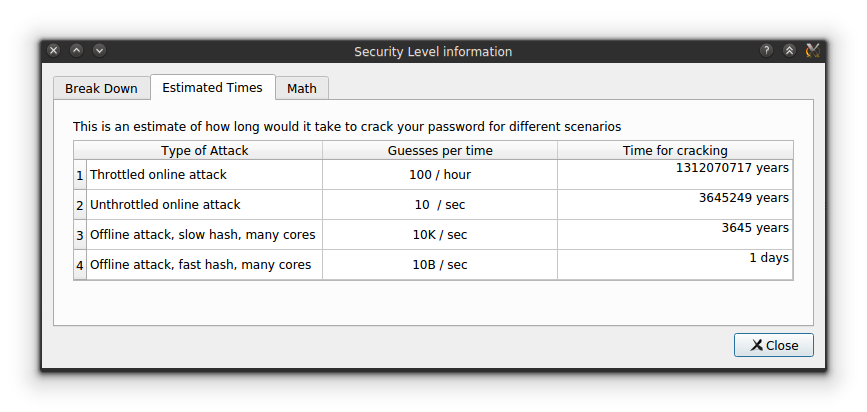
\includegraphics[width=1\columnwidth]{chapters/figures/development/zxcvbnTimes}
  \caption{Crack times for different attacker capabilities}
  \label{fig:zxcvbnTimes}
\end{figure}

Some interesting additional information can be obtained from \texttt{ZxcMatch\_t ** Info}. By traversing the data in this pointer, it is possible to see how the zxcvbn algorithm broke down the password. The user can see this information in a table like the one in figure \ref{fig:zxcvbnBreak}
\begin{figure}[htb]    
  \centering
  \captionsetup{justification=centering}
  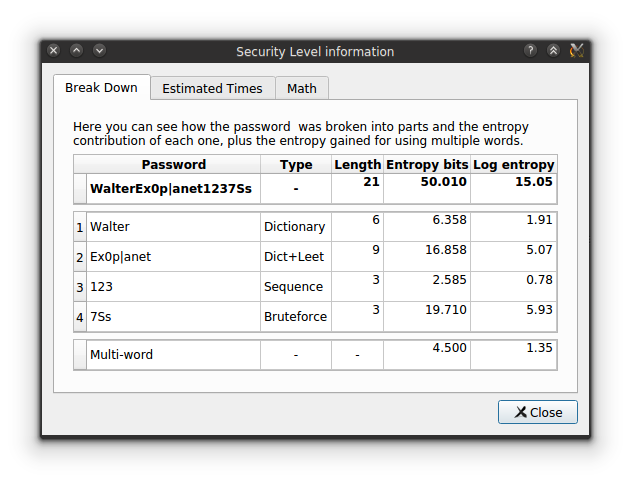
\includegraphics[width=0.9\columnwidth]{chapters/figures/development/zxcvbnBreak}
  \caption{Password broke down by the zxcvbn algorithm}
  \label{fig:zxcvbnBreak}
\end{figure}



\subsection{PassPhrase Generator} \label{sec:ppgen}

The \texttt{PassPhraseGen} C++ function implements the PassPhrase Generator. The function call is done from the \texttt{AddEntry} class, when the \texttt{Generate Password} button is clicked.

\texttt{AddEntry} reads the configuration values stored as \texttt{QSettings}, asserts them and then makes the call. This values can be modified by the user in the preferences window, shown in figure \ref{fig:ppgenSett}. After the user selects the dictionaries and tunes the available options, they must click the apply button, which will trigger a line by line read of the dictionaries, to count the number of lines, that is the number of words available. This is necessary as it is not possible to know how many lines a file has without counting them, and the total number is required in order to generate properly bounded random numbers in the PassPhraseGen function.

\begin{figure}[htb]
  \centering
  \captionsetup{justification=centering}
  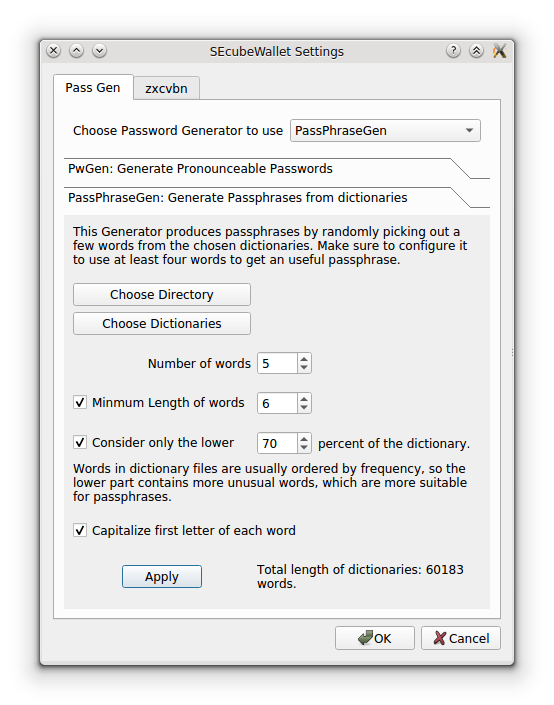
\includegraphics[width=0.8\columnwidth]{chapters/figures/development/ppgenSett.png}
  \caption{Settings for PassPhrase Generator}
  \label{fig:ppgenSett}
\end{figure}

The function declaration is shown in listings \ref{lis:ppgen}


\begin{lstlisting}[style=customc, float=htb, caption={PassPhraseGen function declaration}, label = {lis:ppgen}]
QString PassPhraseGen(  //Return: Generated PassPhrase
  QString path,         //path to dicts
  QStringList dicts,    //list of dicts
  QStringList dictsLen, //cumulative list of dics lengths
  int totalLen,         //total number of candidate words
  int numWords,         //number of words in the password
  bool ppgenMinLenEnab, //use only words longer than min len
  int ppgenMinLen,      //min length
  bool capFirst,        //uppercase first letter of each word
  bool ppgenLowerEnab,  //use only lower part of dicts
  int ppgenLower        //how much of the lower part to use
);
\end{lstlisting}

The function first generates \texttt{numWords} random numbers in the range \texttt{[1, totalLen]} with the Qt function \texttt{QRandomGenerator} (introduced in version 5.10). The generated numbers represent \textsl{Line numbers} in the dictionary files. As each line contains a word, the function indeed extracts random words. There are a few things to consider in this process:
\begin{enumerate}
\setlength\itemsep{-3pt}

\item It is impossible to read a random line from a TextFile without reading all the previous lines first. So, in order to extract the words it is necessary to read the dictionary line by line and keep a counter to know the number line we are at. To speed up the process making sure each line is read only once, the random numbers are sorted in ascending order first. The dictionary can then be read line by line extracting the words where the counter equals one of the random numbers. When the last random line is extracted, the file can be closed.

\item There can be multiple dictionaries. The generated random numbers span the total of available words, so some random lines will be in some dictionaries, some in others. Therefore, using the \texttt{dictsLen} list, which contains the cumulative lengths of the dictionaries, we need to determine in which dictionary and in which internal line, each random number is. With this information, and the random numbers ordered, it is possible to extract the words efficiently and making sure dictionary files are opened only if necessary and only once.

\item When the minimum length option is enabled, the total number of available words is reduced. The algorithm accounts for this fact by counting only the lines with a word larger than the minimum length. This is done both in the preference window, where the total number of lines is counted, and at the word extraction process. In this way, the random lines are pinpointed as before, by reading line by line and comparing the counter; the working logic is not altered, it just ignores the "disabled" short lines.

\item Finally, to consider only the lower part of each dictionary the preferences window counting process is not altered, and the modifications are all done at the extraction process. If for example, the user wants to work with the lower 30\%, the random generated numbers are now bounded to \texttt{[1,  (0.3)totalLen]}. The corresponding dictionary and internal line for each random number are calculated by taking into account that the first 70\% of each dictionary must be skipped. With this two values, the files can be read as in the simple case. As this process is different from the minimum length one, they do not interfere with each other.

\end{enumerate}

Table \ref{tab:ppgenExm} presents some PassPhrases examples for different configurations, along side the score given by the zxcvbn estimator. The estimator uses the same dictionaries as the generator, so this assumes a worst case scenario where the hacker has access to all the possible words the user considered when creating the PassPhrase.

Two dictionaries where used: \texttt{words-eng\_wiki.txt} with 100000 lines and \texttt{words-it\_badip.txt} with 15480 lines (around 6 times smaller), so most of the extracted words will be English.

\begin{table}[ht]
\renewcommand{\arraystretch}{1.3}
\centering
\caption{PassPhrases examples for different configurations}
\begin{tabular*}{\columnwidth}{
@{\extracolsep{\fill}}
m{6.5cm}cccr
@{}}
\toprule
\hd{PassPhrase} & \hd{No. of \\ words} & \hd{Min.\\word \\ Len} & \hd{\% of \\ dict.\\ used } &\hd{Log \\ Entropy \\ \& Level}\\ \midrule

		 Cocchio & 1 & - & - & 4.27 (L1) \\ 
		 Melun   & 1 & - & - & 4.93 (L1) \\ 
		 
		 Legitimately & 1 & 8 & - & 4.55 (L1) \\
     
     Woodhaven		& 1 & 8 & 30\% & 4.94 (L1) \\
     \midrule
     VestaOrman    & 2 & - & - & 7.78 (L2) \\    
     ShorelineCech & 2 & - & - & 9.18 (L3) \\
     
     MongoliaSimpsons & 2 & 8 & -    & 7.30 (L2) \\
     McinnisPhaya     & 2 & - & 30\% & 9.14 (L3) \\

     ZucchiniSalamandra & 2 & 8 & 30\% & 9.19 (L3) \\
     SacchettiVigevano  & 2 & 8 & 30\% & 9.11 (L3) \\

     DrammaturgicoSbatacchiare  & 2 & 12 & - & 8.98 (L3) \\
     MalformationsAstrophysical & 2 & 12 & - & 9.60 (L3) \\
     \midrule
     LatinaInterchangeFbo & 3 & - & - & 13.5  (L4) \\
     OsaAymanCantinflas   & 3 & - & - & 12.98 (L4) \\
     ImmobileCwSites      & 3 & - & - & 11.43 (L4) \\
     
     RimmelBragFaenza     & 3 & - & 30\% & 13.49 (L4) \\
     
     RecliningCanberraEcuadorian         & 3 & 8 &  -   & 13.69 (L4) \\
     
     
     SeashellsHippocraticCameroun        & 3 & 8 & 30\% & 14.90 (L4) \\
     InaspettatoRothschildsDisconcerting & 3 & 8 & 30\% & 14.48 (L4) \\
\bottomrule
\end{tabular*}
		\label{tab:ppgenExm}
\end{table}

The results in the table indicate the most important parameter is the number of words. Three words are enough to reach a zxcvbn level 4, which, as seen in previous sections, is very secure. A two word PassPhrase as long as \texttt{DrammaturgicoSbatacchiare} is not better than the shorter \texttt{ImmobileCwSites}, because the latter has one more word. The minimum word length also influences the PassPhrase entropy, but their effects are not as pronounced. Finally, working only with to the lower part of the dictionary may seem to not have any effect, but in reality its use is crucial: it ensures the generated PassPhrases do not contain any of the most common words, like \texttt{the} or \texttt{essere}. From the results on the table we can not appreciate this fact, but at least we learn the option does not do any harm either. (Although if the attacker finds out the user is generating PassPhrases using only the 30\% most uncommon words on a given language, their job would get easier).


\subsection{The FAT32 bug} \label{sec:fat32bug}
During the application development a strange and elusive bug was found: The \texttt{secureSQLite} library did not work properly with the FAT32 file system. When the save directory was in a FAT32 system, (either a partition, an external hard disk or an USB stick), the created databases were not stored properly, and when trying to open them they were completely empty. Only the database name was saved; any table in the wallet was lost. Moreover, after saving, besides the \texttt{.sqlite} file, a \texttt{.sqlite-journal} was created. Figure \ref{fig:fat32} depicts the presences of this file in a FAT32 file system.

\begin{figure}[htb]
  \centering
  \captionsetup{justification=centering}
  \centerline{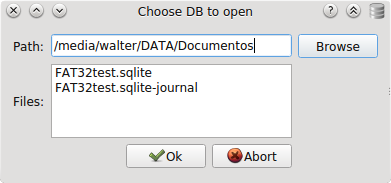
\includegraphics[width=0.55\columnwidth]{chapters/figures/development/fat32.png}}
  \caption{secureSQLite Databases in a FAT32 file system}
  \label{fig:fat32}
\end{figure}

This file is known as a rollback journal and is used by the SQLite standard to avoid database corruption when a transaction can not be completed. From the SQLite official documentation \cite{journal}:
``The rollback journal is always located in the same directory as the database file and has the same name as the database file except with the 8 characters "-journal" appended. The rollback journal is usually created when a transaction is first started and is usually deleted when a transaction commits or rolls back. The rollback journal file is essential for implementing the atomic commit and rollback capabilities of SQLite. Without a rollback journal, SQLite would be unable to rollback an incomplete transaction, and if a crash or power loss occurred in the middle of a transaction the entire database would likely go corrupt without a rollback journal.
The rollback journal is usually created and destroyed at the start and end of a transaction, respectively. But there are exceptions to this rule.
If a crash or power loss occurs in the middle of a transaction, then the rollback journal file is left on disk. The next time another application attempts to open the database file, it notices the presence of the abandoned rollback journal (we call it a "hot journal" in this circumstance) and uses the information in the journal to restore the database to its state prior to the start of the incomplete transaction.''

The presence of the journal file hints at the problem being an interruption during the execution of \texttt{secureSQLite} write functions when working on a FAT32 system. A few test were performed to try to narrow down the error origin:

\begin{itemize}
\setlength\itemsep{-3pt}

\item The application was tested in other computer running a different OS, and the problem persisted, always in FAT32 systems, meaning it was not an OS specific issue.
\item The application \texttt{secureSQLiteBrowser} which also uses the secureSQLite library was tested and presented the same problem, meaning it was not an error in the library usage.
\item The demo applications \texttt{SEfile\_IMG}  and \texttt{SEfile\_TXT} were also tested, and worked without any problems in FAT32 partitions. These applications do not use \texttt{secureSQLite}; they leverage directly the \texttt{SEfile} library, which is also used by the \texttt{secureSQLite} library, meaning the problem was not in \texttt{SEfile} but in \texttt{secureSQLite}. This was proved to be a wrong assumption later on.
\end{itemize}

With these points in mind, the bug was searched inside the \texttt{secureSQLite} library, but after several debug sessions, it was possible to trace the error origin to the \texttt{SEfile} library. Specifically, in the file \texttt{SEfile.c}, and function \texttt{secure\_seek}. Figure \ref{fig:traceback} shows the actual traceback, from the call to \texttt{sqlite3\_exec} in the \texttt{Save\_Wallet} action, all the way up to the \texttt{secure\_seek} function.

\begin{figure}[htb]
  \centering
  \captionsetup{justification=centering}
  \centerline{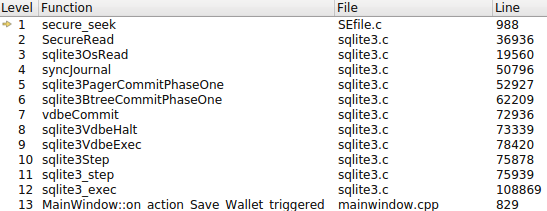
\includegraphics[width=0.8\columnwidth]{chapters/figures/development/traceback.png}}
  \caption{Error Traceback}
  \label{fig:traceback}
\end{figure}

The actual error is produced in the call to the OS function \texttt{lseek()} in line \ref{line:error} of listing \ref{lis:secseek}. 
\begin{lstlisting}[style=customc, float=htb, caption={FAT32 Error origin at secure\_seek}, label = {lis:secseek}, escapechar=¬]
/**This function is used to move correctly the file pointer.
 * [in]  hFile     The handle to the file to manipulate.
 * [in]  offset    Amount of character we want to move.
 * [out] position  Pointer to int32_t to store the final pos.
 * [in]  whence    Move from file start, end or current pos.
 * [return]        Returns '0' in case of success.*/
uint16_t secure_seek(SEFILE_FHANDLE *hFile, int32_t offset, int32_t *position, uint8_t whence){
  ...  
  buffer_size = *position - file_length;
  if(buffer_size>0){ ¬\label{line:buffer}¬
    //if destination exceed the end of file, empty sectors are inserted at the end to keep the file consistency
    buffer=calloc(buffer_size, sizeof(uint8_t));
    if(buffer==NULL)
      return SEFILE_SEEK_ERROR;
    
    if((file_length%SEFILE_LOGIC_DATA)){
      errno = 0; //clear errno 
      hTmp->log_offset=lseek( // the error is produced here ¬\label{line:error}¬
        hTmp->fd, 
        ((file_length%SEFILE_LOGIC_DATA)-SEFILE_SECTOR_SIZE), 
        SEEK_END);
      error = errno;//capture errno, 22 when in FAT32 systems
      if(hTmp->log_offset==4294967295)
        //lseek returns (off_t)-1 when error. off_t is 32 bits, so 2^32-1 = 4294967295
        return SEFILE_SEEK_ERROR; //the upcoming secure_write call fails anyway
      
      if(secure_write(&hTmp, buffer, buffer_size)){
        free(buffer);
        return SEFILE_SEEK_ERROR;
      }   
\end{lstlisting}

\vspace{15pt}
The \texttt{lseek()} function, as defined in the linux manual page \cite{lseek}:

\texttt{\textcolor{blue}{off\_t} lseek(\textcolor{blue}{int} fd, \textcolor{blue}{off\_t} offset, \textcolor{blue}{int} whence);}

``\textbf{\texttt{lseek()}} repositions the file offset of the open file description
       associated with the file descriptor \texttt{fd} to the argument \texttt{offset}
       according to the directive \texttt{whence} as follows:
       
       \texttt{SEEK\_SET} The file offset is set to offset bytes.
       
       \texttt{SEEK\_CUR} The file offset is set to its current location plus offset bytes.
       
       \texttt{SEEK\_END} The file offset is set to the size of the file plus offset bytes.
lseek() allows the file offset to be set beyond the end of the file
       (but this does not change the size of the file)
       
\textbf{Return Value:} Upon successful completion, \texttt{lseek()} returns the resulting offset
location as measured in bytes from the beginning of the file.  On error, the value \texttt{(off\_t) -1} is returned and \texttt{errno} is set to indicate the error.''

\vspace{7pt}
\texttt{secure\_seek()} can be seen as a wrapper that uses the OS function \texttt{lseek()} to move the file pointer correctly, taking into account the way the \texttt{SEfile} library redefines a file, including the overhead added by sectors and headers that allow the data to be encrypted.

\vspace{7pt}       
To better understand what was causing the error, the \texttt{return} and \texttt{errno} values for two save operations of the same database were compared. One into a FAT32 file system and the other into a ext4 system.

When the FAT32 system was used, the \texttt{return} value was indeed \texttt{(off\_t)-1}, and the \texttt{errno}, was set to \texttt{22}, which corresponds to:

``\texttt{EINVAL}:  \texttt{whence} is not valid.  Or: the resulting file offset would be negative, or beyond the end of a seekable device.''

When saving into an ext4 file system, the \texttt{return} value was \texttt{9844} and \texttt{errno} was equal to zero.

\vspace{7pt}
Figure \ref{fig:errordebug} shows this difference, and it is worth noticing that besides the file descriptor and pointers (always different for different executions), the rest of the variables have the same value
\begin{figure}[ht]
  \centering
  \subfloat[FAT32 filesystem\label{}]{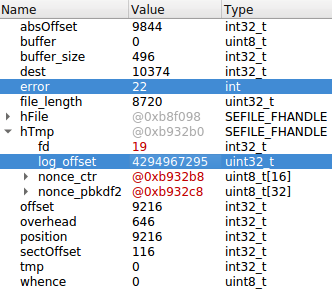
\includegraphics[width=0.48\textwidth]{chapters/figures/development/fat32debug.png}}
  {}
  \subfloat[ext4 filesystem\label{}]{\includegraphics[width=0.48\textwidth]{chapters/figures/development/ext4debug.png}}
  \caption{Return and errno values for a save operation}
 \label{fig:errordebug}
\end{figure}

Going back to the \texttt{secure\_seek()} code in listing \ref{lis:secseek}, the line \ref{line:error} moves the file pointer to the last \texttt{LOGIC\_DATA} byte, because in order to keep the file consistency, its is required to write empty sectors starting from this position until the end of the file. To do so, starting from the end of the file (thus the argument \texttt{SEEK\_END}), the function moves the pointer backwards the number of empty bytes in the last sector.

In order to move backwards, the \texttt{offset} argument of \texttt{lseek()} must be negative. In this case, the argument is equal to: 

\lstset{style=customc}
\lstinline"offset = (file_length%SEFILE_LOGIC_DATA)-SEFILE_SECTOR_SIZE"

Which should always be always negative, but it turns out, in the case of the FAT32 file system, this offset is not interpreted as a 2's complement negative value, but as a very large positive one. Therefore, the \texttt{lseek()} function tries to move the pointer outside the file limit, explaining the error: \texttt{EINVAL}: the resulting file offset would be negative, or beyond the end of a seekable device.

\vspace{7pt}
To fix the error, a simple cast to \texttt{\textcolor{blue}{int32\_t}} for the \texttt{offset} argument is enough, resulting in the call:
\vspace{5pt}

\lstinline|hTmp->log_offset=lseek(|

\lstinline|  hTmp->fd,| 

\lstinline| (int32_t)((file_lengh%SEFILE_LOGIC_DATA)-SEFILE_SECTOR_SIZE),| 

\lstinline|  SEEK_END);|
\vspace{7pt}

This kind of casting was actually found in other function calls in the \texttt{SEfile.c} file, so it made sense to use it in this situation too.

\vspace{7pt}
The reason the problem only affected FAT32 partitions is probably related to the fact that, as \texttt{lseek()} needs to move a file pointer, low-abstraction level functions need to be used, which are have different implementations for each type of file system. The ext4 low level functions were able to interpret the offset as negative whereas the FAT32 took it as positive.

Why the error only appears when using the \texttt{secureSQLite} library, and not in the demo applications \texttt{SEfile\_IMG} and \texttt{SEfile\_TXT} honestly remains a mystery. It may be  that the condition in line \ref{line:buffer} of listing \ref{lis:secseek} (\lstinline|if(buffer_size>0)|), that evaluates if the destination exceeds the end of file, is only met in rare occasions, and the way SQLite journaling works is one of them.

\chapter{Results, Discussion and Future work} \label{chap:res}

In this chapter first an overview of the obtained results is given. Then, some drawbacks of the chosen approach are discussed. Finally a few ideas for future work an improvements are considered.

\section{Results}

The developed application, SEcubeWallet, is a completely functional and reliable hardware-based Password Manager . All of the code is open source, and is hosted in GitHub \cite{secubewallet}.

The application exploits the security-oriented capabilities of the SEcube™ framework, the facilities of the Qt library and the functionalities of a few other open source tools to offer the following features:

\begin{enumerate}
\setlength\itemsep{0pt}
\item Confidence in the safeness of the stored passwords. The user is assured only with the correct device and master password is possible to decrypt the data. Even if an attacker has access to the encrypted files (for instance if the host machine is stolen), it is not possible to even try to hack the master password without the SEcube™ device.
\item The application is very comfortable to use, as the graphical elements used to display and manipulate the passwords are elegant and responsive.
\item The user can search easily for any password item, thanks to the powerful filters, available for each field. Using the date special filter, it is possible to look for expired passwords that need to be updated.
\item The application can suggest passwords suited for any situation, ranging from completely random ones, perfect for machine passwords, to pronounceable passwords and random passphrases, easier to memorize without compromising their strength.
\item If the user wishes to evaluate how strong their current passwords are, they can use the strength estimator, which gives clear information on how the password could be cracked and how long it would take.
\end{enumerate}

Besides the application development, other results obtained during this work are:
\begin{enumerate}
\setlength\itemsep{0pt}
\item The implementation of an improved Login behaviour in the SEcube™ framework, that renders more usable SEcubeWallet and any other application that uses the SEcube™ authentication system.

\item The discovery and fix of a bug in the SEfile library that did not allow to use the secureSQLite library in a FAT32 file system.
\end{enumerate}


\section{Application's drawbacks}
In this section, the drawbacks of the SEcubeWallet application are discussed, as well as some ideas about how to fix them.


\subsection{First table corruption}
As explained in session \ref{sec:savewalletaction}, during the application development it was impossible to find the origin (and solution) to an error concerning the database saving and opening process: the first table in a wallet is always corrupt. The problem is not present when using the regular SQLite API; it only appears when using the secured version. This seems to point out the error is the secureSQLite library's fault. But because the secureSQLiteBrowser application does not have this problem it is not possible to discard SEcubeWallet as the origin of the problem.

The secureSQLiteBrowser and SEcubeWallet applications differ in the way they use the secureSQLite API. secureSQLiteBrowser, as it is a data base manager, uses complex SQLite functionalities like save points and pragma statements to exploit all of the API's capabilities, while SEcubeWallet only uses simple open/exec/close SQLite functions. So in a way SEcubeWallet is responsible for the error that could be avoided by using more complex SQLite statements. But the secureSQLite library should behave as the regular SQLite API, specially in the most simple cases.

In any case, the implemented workaround in SEcubeWallet (always having an unused and empty first table to sacrifice) should be considered temporary, not only because it is not optimal, but more importantly, because the unfixed error may cause other problems in the future.

\subsection{The FAT32 bug}

Even if the FAT32 bug (see section \ref{sec:fat32bug}) can be considered to be fixed, the truth is its origin is not completely clear, and it may be the case the adopted solution (casting to int) only works for a subset of cases.

\subsection{Only Linux has been tested}

The SEcubeWallet application has only been tested running on Linux. Although Qt is platform independent, some of the application functionalities may need some changes to work on Windows or Mac systems. For example, the zxcvbn compilation process relies on gcc commands, that may not be available in Windows. Moreover the FAT32 bug is a very OS specific issue, as it involves the use of the lseek() function (Linux and Mac). It may be the case the bug does not exists in a Windows machine, or on the contrary there are other errors waiting to be fixed.


\subsection{Missing icons}
The reader of this thesis may have noticed the lack of icons in all of the SEcubeWallet Windows. Due to tight time constraints, it was decided to allocate most of the efforts into other aspects of the application, but that is not to say icons are not important. Future version of the application will definitely have icons to increase the user experience.


\section{Future work}
In this section, a few ideas about how to extend the SEcubeWallet functionalities are given. None of them were considered for this work as they are either too time consuming to implement, or are beyond of the author's expertise.


\subsection{SEkey integration}

SEkey is a new library currently under development at Politecnico di Torino by 	Mateus Françani as his master thesis work. The library will sit next to SEfile and SElink, as depicted in Figure \ref{fig:sekey} taken from \cite{sekey}.

\begin{figure}[htb]
  \centering
  \captionsetup{justification=centering}
  \centerline{\includegraphics[width=0.8\columnwidth]{chapters/figures/results/sekey.png}}
  \caption{Host side SEcube™ architecture, including the SEkey library}
  \label{fig:sekey}
\end{figure}

The library will work as a key management system for the SEcube™ framework. Right now keys inside a SEcube™ chip can only be modified at factory reset. This is not very useful in a working environment, as the purpose of having multiple keys is to allow users to share information with selected people (people sharing a key are known as a group). The job of the SEkey library will be to allow an administrator to dynamically add and remove keys to SEcube™ devices using an intuitive GUI. By doing so, the administrator can conform groups of users, that later on can use their SEcube™ devices to share sensitive information, knowing it will be secured against unauthorized access (from people outside the group).

As the SEcubeWallet application already offers an intuitive GUI for the management of passwords, it could be extended to support the management of keys as well. If the person login in is an administrator, the application should offer the possibility to edit the keys present in the SEcube™ device. If it is a regular user, it should only let them see what keys they can use, i.e. to which groups they belong.

\subsection{Browser integration} 

The vast majority of users store their internet passwords within their preferred web browser, alongside other sensitive information like browsing history and bookmarks. This allows them to use their passwords easily and fast, as they can for example autofill login credentials in websites.

Exploit the capabilities of the SEcube™ platform to protect all that information and allow to autofil logins, while maintaining ease of use and transparency to the final user would be a great advance in the purpose of reaching as many users as possible.

A couple of alternatives come to mind in order to implement this integration:
\begin{itemize}
\setlength\itemsep{-3pt}

\item Borrow the idea followed by the Mooltipass system, porting the entire Qt application to a complement for the most popular web browsers (Firefox, Chrome, Opera).
\item Implement a web browser complement that "talks" with the SecubeWallet application and request for passwords when the user wishes to autofill a login field.
\item Follow the auto-type approach used by the software password manager KeePass. \cite{autotype}. ``KeePass features an "Auto-Type" functionality. This feature allows you to define a sequence of keypresses, which KeePass can automatically perform for you. The simulated keypresses can be sent to any other currently open window of your choice (browser windows, login dialogs, ...). By default, the sent keystroke sequence is \{\textsc{username}\} \{\textsc{tab}\} \{\textsc{password}\} \{\textsc{enter}\}, i.e. it first types the user name of the selected entry, then presses the Tab key, then types the password of the entry and finally presses the Enter key.''
\end{itemize}

In either case ensuring the new functionalities do not compromise the security of the passwords must be the top priority.

\subsection{More than just static Passwords}
Other authentication methods besides static passwords have been gaining popularity over the past two decades, among them One-Time passwords and FIDO U2F. An interesting line of work could be supporting these standards by using the capabilities of SEcube™ to extend the functionalities of the wallet.

\subsection{Hardware button on SEcube™ device}
A recurring interesting idea in many hardware-based password managers is the presence of a hardware button in the  device the user has to press in order to allow any critical operation (Login, password decryption) to be completed. This idea could be implemented in the SEcube™ DevKit, as it has multiple buttons. Unfortunately, the USEcube™ Stick does not.

\subsection{Mobile application (Android)}
To have a functional SEcubeWallet for the Android system, three elements would need to be ported:
\begin{itemize}
\item The SEcube™ chip. As far as the author knows, the Blu5 group is working on a product that would allow to use the SEcube™ hardware platform in smartphones running the Android OS.
\item The software libraries. The SEfile and secureSQLite libraries are written to work on Linux, Windows and Mac systems. Given that Android is based on Linux, porting the libraries should be possible.
\item The GUI. Qt for Android \cite{android} ``allows to run Qt 5 applications on devices with Android v4.1 (API level 16) or later''. All of the Qt modules used by SEcubeWallet are supported, but a GUI redesign is required in order to cope with the constraints imposed by a smaller display.
\end{itemize}

\subsection{Eliminate dependability on the OS}

The application relies heavily on the operating system's memory protection feature to ensure no other process can access its private data and steal the passwords while they are opened and temporary stored in the application's memory space. An interesting path of research is how to eliminate this dependency, or at least decrease it, using the SEcube™ encryption capabilities.

\subsection{Custom columns}

Wallets in the SEcubeWallet application have a fixed set of columns (\textsc{username}, \textsc{domain}, \textsc{password}, \textsc{description}, \textsc{date}). This set should be enough in most of the cases as they are the standard for wallet managers, but some users may want to add other custom columns, for instance to store "security questions and answers" used by some websites, an email associated to the account, or multiple passwords in the same entry.

\subsection{Expired passwords notification}

Changing passwords regularly is important to keep a high level of security in any system. If the user has a large number of passwords it may be hard to remember when one of them needs to be updated. SEcubeWallet already offers the possibility to search for passwords older than a given period of time (for example passwords older than six months). This functionality could be extended to notify the user when a password needs to be updated. The user could configure the expiration time for each password individually, or for all of them, and how they wish to be notified (Message inside the application, desktop notification, email, etc).
\chapter{Conclusions} \label{chap:con}

The followed approach and the chosen set of hardware and software libraries proved to be more than appropriate for the implementation of a secure hardware-based password manager.

\vspace{7pt}

The SEcube™ framework is robust enough to offer all the necessary tools for reliable encryption of data, and the set of custom software libraries allow developers non experts in cryptography to design and implement any security related application. A project like the one explained in this work requires knowledge in several fields, mainly embedded programming, digital security and front end development. The well defined levels of abstraction given by the software libraries allow to easily combine the expertise of a group of developers to create any desired application.

\vspace{7pt}

The use of the Qt library did not led to any shortcomings or compatibility problems. On the contrary because it is C++ based, is an excellent choice for the development of applications making use of embedded devices and C libraries. Additionally, all the high level wrappers hiding low level functions and OS calls result in an easier and less error prone programming, and in a cross-platform application.

\vspace{7pt}

In any password manager it is important to provide a tool to suggest random passwords, because humans are inherently bad at generating really random information, that guarantees the security of the protected system. However, to increase the user experience, it is also desired to have the possibility of less-random more memorable passwords. It is equally important to check the validity of said passwords by using an appropriate metric, for instance their entropy, because even random generated passwords can end up being too guessable

\vspace{7pt}

All the used libraries in this project are open source, proving it is possible to achieve a high level of security with the use of open software and hardware tools. The biggest concern customers have when choosing a new security related product is whether or not they can trust the designers, both in their ethics and in their knowledge. Using open source platforms solve this issue, as it allows the community to critically review the products for accidental or intentional security flaws. There are already in the market similar products to SEcubeWallet in terms of purpose, but none of them offers the combination of completely open source hardware and software, and the reliability of a mature and tested framework as the SEcube™.

\vspace{7pt}

The developed application still lacks some features in order to be considered a truly commercial product. Among them, the support for other authorization standards (One Time Passwords, FIDO U2F) already offered by other hardware password managers. Moreover, security can not be the only goal, as users also look for the product offering the most comfortable experience, and want the transition from software to hardware managers to be as seamless as possible. So ideally, all the features already offered by software managers should also be supported. A first step in this direction is the possibility to auto complete login forms in websites without compromising the security of the system.

\bibliographystyle{acm}
\bibliography{references}


\end{document}


